\documentclass[11pt,twoside]{report}


\usepackage{fixltx2e} % LaTeX patches, \textsubscript
\usepackage{cmap}    % fix search and cut-and-paste in Acrobat
\usepackage{ifthen}
\usepackage[T1]{fontenc}
\usepackage[utf8]{inputenc}
%\usepackage{amsmath}
\usepackage{amsmath, amsthm, amssymb, amsbsy}
\usepackage{newtxtext,newtxmath}
%%% Custom LaTeX preamble
% PDF Standard Fonts
\usepackage{helvet}
\usepackage{courier}
\usepackage{graphicx}
\usepackage{textcomp}
\usepackage{natbib}
\usepackage{mathtools}
\usepackage{hyperref}
\usepackage{etoolbox}
\renewcommand{\bibname}{References}
\apptocmd{\thebibliography}{\csname phantomsection\endcsname\addcontentsline{toc}{chapter}{\bibname}}{}{}



%\usepackage{fullpage} deprecated
\usepackage[left=1.25in,right=1.2in,vmargin=1.2in,headheight=110pt]{geometry}

\usepackage{enumitem}
%\setlist{nolistsep}

% header setup
\usepackage{fancyhdr}
\pagestyle{fancy}
\fancyhf{}
\fancyhead[LO]{Bay-Delta SELFE v1}
\fancyhead[LE]{Bay-Delta SELFE v1}
\fancyhead[RO]{\leftmark}
\fancyhead[RE]{\rightmark}
\fancyfoot[CE,CO]{\thepage}
\renewcommand{\headrulewidth}{0.4pt}

\hypersetup{
    colorlinks,
    citecolor=black,
    filecolor=black,
    linkcolor=black,
    urlcolor=black
}

\usepackage[acronym,toc,nomain]{glossaries}
\newglossary[slg]{symbols}{sym}{sbl}{List of Symbols}
\makeglossaries

\newacronym{selfe}{SELFE}{Semi-implicit, Eulerian-Lagrangian Finite Element Model}
\newacronym{cmop}{CMOP}{Center for Marginal Ocean Prediction}
\newacronym{vims}{VIMS}{Virginia Institute of Marine Science}
\newacronym{vof}{VoF}{Volume of Fluid}
\newacronym{fem}{FEM}{Finite Element Method}
\newacronym{elm}{ELM}{Eulerian-Lagrangian Method}
\newacronym{les}{LES}{Large Eddy Simulation}
\newacronym{gotm}{GOTM}{General Ocean Turbulence Model}
\newacronym{ctd}{CTD}{Conductivity-Temperature-Depth}
\newacronym{bdcp}{BDCP}{Bay-Delta Conservation Plan}
\newacronym{nmfs}{NMFS}{National Marine Fisheries Service}
\newacronym{cfl}{CFL}{Courant–Friedrichs–Lewy}
\newacronym{usbr}{USBR}{U.S. Bureau of Reclamation}
\newacronym{dwr}{DWR}{California Department of Water Resources}
\newacronym{d1641}{D1641}{California Water Rights Decision 1641}
\newacronym{psu}{PSU}{Practical Salinity Unit}
\newacronym{ec}{EC}{electric conductivity}
\newacronym{doc}{DOC}{Dissolved Organic Carbon}
\newacronym{ndo}{NDO}{Net Delta Outflow}
\newacronym{dsm2}{DSM2}{Delta Simulation Model 2}
\newacronym{dcc}{DCC}{Delta Cross Channel}
\newacronym{uvm}{UVM}{Ultrasonic Velocity Meter}
\newacronym{adcp}{ADCP}{Acoustic Doppler Current Profiler}
\newacronym{cwemf}{CWEMF}{California Water and Environmental Modeling Forum}
\newacronym{ebmud}{EBMUD}{East Bay Municipal Water District}
\newacronym{ccwd}{CCWD}{Contra Costa Water District}
\newacronym{swp}{SWP}{State Water Project}
\newacronym{cvp}{CVP}{Central Valley Project}
\newacronym{ccfb}{CCFB}{Clifton Court Forebay}
\newacronym{bbid}{BBID}{Byron Bethany Irrigation District}
\newacronym{dfd}{DFD}{Delta Field Division}
\newacronym{cencoos}{CenCOOS}{Central and Northern California Ocean Observing System}
\newacronym{coamps}{COAMPS}{Coupled Ocean-Atmosphere Mesoscale Prediction System}
\newacronym{narr}{NARR}{North American Regional Reanalysis}
\newacronym{tvd}{TVD}{Total Variation Diminishing}
\newacronym{detaw}{DETAW}{Delta Evapotranspiration of Applied Water}
\newglossaryentry{elev}{type=symbols,name=elev,symbol={\eta},description={Free surface elevation or stage}}


%%% User specified packages and stylesheets


%%% Macros
\newcommand{\pd}{\partial}
\newcommand{\beq}{\begin{equation}}
\newcommand{\beqa}{\begin{eqnarray}}
\newcommand{\eeq}{\end{equation}}
\newcommand{\eeqa}{\end{eqnarray}}
\newcommand{\mi}{\mbox{i}}
\newcommand{\kp}{\kappa}
\newcommand{\md}{\mbox{d}}
\newcommand{\bs}{\boldsymbol}
\newcommand{\ba}{\begin{array}}
\newcommand{\ea}{\end{array}}
\newcommand{\subphi}{\textsubscript{$\phi$}}
\providecommand{\D}{\Delta}
\providecommand{\nn}{\nonumber}
\newcommand{\sgn}{\operatorname{sgn}}
\DeclareMathOperator*{\Max}{Max}
\DeclareMathOperator*{\Min}{Min}

%%% Fallback definitions for Docutils-specific commands

\title{Bay-Delta SELFE}
\author{Eli Ateljevich,\\Kijin Nam,\\Yinglong Zhang}
%%% Body
\begin{document}
\maketitle
\thispagestyle{empty}

\newcommand{\explain}[2]{\underset{\mathclap{\overset{\uparrow}{#2}}}{#1}}
\newcommand{\explainup}[2]{\overset{\mathclap{\underset{\downarrow}{#2}}}{#1}}



\tableofcontents

\chapter{Introduction}
This document describes the first calibration of the three dimensional \gls{selfe}
on the Bay-Delta, performed collaboratively by the California Department of Water Resources 
and the Virginia Institute of Marine Sciences. The main items of discussion will be the scope of the Bay-Delta SELFE effort, 
the assumptions and additions made for the domain, initial calibration and validation results, 
and a statement of suitability for various types of current and future studies. 

Our goal for the initial calibration was to accurately illustrate and answer operational and planning 
questions involving multidimensional flow and constituent transport in the Bay-Delta system
over periods of months or years. This goal requires that we accurately resolve the principle mechanisms of multi-dimensional transport up the estuary and in Delta channels: 
gravitational circulation, tidal trapping, pumping and flood-ebb asymmetry. In many cases it also requires that the model
be reconfigurable in a {\em near field - far field} arrangement whereby a higher resolution regions of focus is nested 
within the coarser, pre-calibrated grid connecting the study region to the rest of the system.

At the time of writing the following are the motivating applications for our work:

\begin{itemize}
	\item \gls{bdcp} mandated habitat restoration and island flooding
  \item Local changes in velocity patterns caused by tunnel intakes or receiving sections of the Clifton Court Forebay.
	\item The effects of sea level rise, climate change and storm surge in the Delta
  \item Yolo Bypass fish passage
  \item Mercury fate in Liberty Island, Yolo Bypass and the Delta
  \item Full life cycle modeling of salmon (collaboration with NMFS and NASA)
\end{itemize}

In terms of resolution and detail, many of these applications share two common requirements. First the model 
must capture variation of the mean flow field over the cross section (net of turbulence). 
Second, many of these applications require local regions of local refinement or additional physics. 

SELFE is a three-dimensional, cross-scale hydrodynamic and transport model capable of modeling flow, water quality, 
temperature and particle trajectories over scales ranging from oceanic to fairly small channels. 
Its meshing is of the "unstructured"' type (see section***), allowing it to flexibly conform 
to natural bathymetry and making it amenable to near-field regions of focus. The SELFE 
community has coupled or built modules for sediment transport, wind-wave 
interaction, oil spills, biogeochemistry and particle transport (Figure ***). While features from a generic modeling suite usually
need to be adjusted to fit the sources, sinks and interactions of the San Francisco Bay-Delta systems, 
these modules represent a significant head start tackling multidisciplinary problems.  
Two of our ongoing projects are of this multidisciplinary nature: 
the salmon life cycle model collaboration with NMFS and NASA includes flow, temperature, food production and fish travel; 
The Methylmercury project involves specific chemistry as well as sediment/detritus interaction. 

The current calibration document, however, focuses on tide propagation and salinity transport. The reasons for focusing on salt are well-known. 
First, salinity intrusion is still by far the most important water quality issue facing the water projects and salt (or rather conductivity) 
is extensively monitored at stations throughout the estuary. Second, the processes giving rise to mixing are very similar 
for any diffuse, conservative tracer. The ability to model the circulation of salt is likely to predict fidelity on other constituents such as  ***. 

The remainder of this document explores the range of applicability further by the Bay-Delta calibration. The purpose of calibrating a 
hydrodynamic model is to ready the model for a new domain or application, adjust parameters and gain insight
into the model suitability for various operational and planning purposes. Calibration is always indicated for a new model application; 
it may also be needed when new physical processes (sediment, biogeochemistry) are added or when new data becomes available. 
This insight can then be better quantified by validating over a longer period in which the model is not adjusted or fit to the data. 

Chapter  *** describes the SELFE model formulation and features, including two capabilities developed for this project: 
subgrid hydraulic structures to model Delta gates and barriers and mass sources and sinks to model island diversions and returns. 
Chapter *** describes the model configuration and assumptions and configuration of the general Bay-Delta application. Chapters *** and *** respectively detail model calibration and validation results. Chapter ** summarizes these results into statements of suitability we think we have
established for the model, and gives a description of ongoing work in certain more specific (and more multidimensional) metrics of suitability that will pertain to subjects such as secondary circulation and mercury cycling on partial island flooding.

We hope this Version 1 calibration will establish a suitable benchmark of progress to date and the suitability of the model for numerous applications.



 

\chapter{SELFE Model}
\label{chap:selfe}
\section{Introduction}
\section{SELFE suite of tools}
The \acrfull{selfe} \citep{Zhang08} is a cross-scale 3D shallow water open source hydrodynamic model jointly 
developed by \acrfull{cmop} and \acrfull{vims}.

The main variables calculated by SELFE are the elevation of the free surface (stage), 
three-dimensional velocity and concentrations of salinity,
temperature and other scalar concentrations (only salinity is considered in this calibration), as well as turbulent quantities. Extensions in the SELFE suite use the flow field to calculate particle trajectories, sediment transport and nutrient availability. The input required by SELFE includes the initial state of the system and boundary time series
 representing fluxes and water surfaces at all the open boundaries. 

The underlying computational engine SELFE is a second-generation semi-implicit model sharing some of the 
algorithmic background of the \cite{Casulli99} family of models, which also includes UnTRIM and SUNTANS that have been
used before with some success on the Bay. SELFE's predecessor, ELCIRC \citep{Zhang04}, was perhaps the first open source model of this class to receive wide distribution. SELFE was devised to improve the depiction of 
bathymetry and salinity plume transport in realtime applications in the Columbia River region. 
SELFE shares some code with ELCIRC, but its discretization and solution scheme includes some 
innovations that make it more formally accurate. SELFE has also been parallelized and used by groups all over the world on a diverse
variety of high performance computers.

\begin{figure}
	\centering
		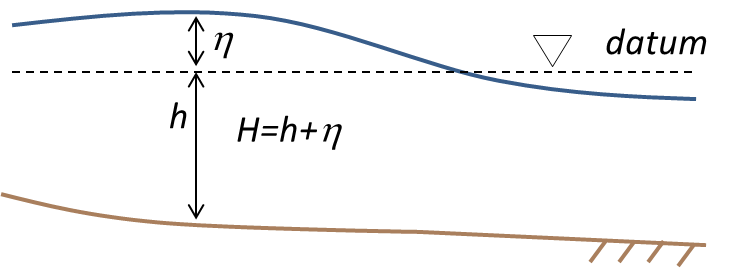
\includegraphics[scale=1.0]{image/depth_definition}
	\caption{Definition of bathymetric depth ($h$), elevation ($\eta$) and total depth ($H$) as used in SELFE.}
	\label{fig:depths}
\end{figure}

\section{Formulation}
\subsection{Equations of motion}\label{sec-1}
The formulation of SELFE is based on classic expressions of mass and momentum conservation within a shallow fluid,
as well as the transport equations for salt and heat. The three dimensional expressions of these laws of motion
involve much less reduction and averaging than one or two-dimensional models. However, 3D estuary-scale models
do invoke a standard set of assumptions that will be discussed in section \ref{sec-assump}.

The SELFE variant used in this equation is defined in a Cartesian (ie map projection) frame with
bathymetric depth $h$ and free surface $\eta$ defined relative to a fixed datum (NAVD 88 in our case) as shown 
in Figure \ref{fig:depths}. The total depth $H$ is the sum of bathymetric depth and free surface elevation.



The 3D continuity, depth-integrated mass conservation, and horizontal momentum conservation equations are given by:
\begin{align}
  %& \text{3D Continuity}& \nonumber \\
  \nabla \cdot \bs{u} &= 0 \label{3Dcon}&\\
  %& \text{Depth-integrated Continuity}& \nonumber \\
  \eta_t+\nabla \cdot \int_{-h}^\eta \bs{u} & = 0 \label{cont1} &\\
  %& \text{Momentum}& \nonumber \\
  \frac{D\bs{u}}{Dt} &= \explain{ -f\bs{k} \times \bs{u} }{\text{Coriolis}} 
	                      \; \explain{-\frac{1}{\rho_0} \nabla p_A}{\text{Atmos. pressure}}
												\; \explain{- \frac{g}{\rho_0} \int_z^\eta \nabla \rho d \xi}{\text{Baroclinic}}
	                      \; \; \; \explain{-g\nabla \eta}{\text{Gravity wave}} & \nonumber \\
	                      \; \; \; &\explain{+ \nabla \cdot (\mu \nabla \bs{u})}{\text{Horizontal diffusion}}
												\; \; \; \; \explain{+\frac{\pd}{\pd z}(\nu \frac{\pd \bs{u}}{\pd z})}{\text{Vertical diffusion}} \label{mom1}
	\end{align}
	with wind and bed stress boundary conditions at the surface and bottom of the water column:
	\begin{align}
	\nu \frac{\pd \bs{u}}{\pd z} &= \bs{\tau}_w \mbox{ at } z=\eta &\\
  \nu \frac{\pd \bs{u}}{\pd z} &= \chi \bs{u}_b \mbox{ at } z=-h &
\end{align}
where the variables and parameters are:
\begin{align*}
&\eta(x,y,t)  &\text{free surface elevation (m)} &\\
&\bs{u}(x,y,z,t)  &\text{horizontal velocity(m/s)}  &\\
&h(x,y)  &\text{bathymetric depth(m)} &\\
&w  & \text{vertical velocity (m/s)}  &\\
&f     & \text{Coriolis factor (s\textsuperscript{-1} )} & \\
&g     & \text{gravity (m/s\textsuperscript{2})} & \\
&\rho  & \text{water density (kg/m\textsuperscript{3})} & \\
&p_A(x,y, t) & \text{atmospheric pressure at the free surface (N m\textsuperscript{2})} & \\
&\nu    & \text{vertical eddy viscosity (m\textsuperscript{2}/s)} & \\
&\mu    & \text{horizontal eddy viscosity (m\textsuperscript{2}/s) }\\
&\kappa & \text{vertical eddy diffusivity, for salt and heat (m\textsuperscript{2}/s)} & \\
\end{align*}

and the labeled processes in the momentum equations include:
\begin{description}
    \item{Coriolis} an apparent force that results from writing equations on a rotating system (the earth) in a projected (x,y) coordinate system. The Coriolis force is most important in the ocean and near coast, less so in estuary or riverine systems. 
	  \item{Atmospheric pressure} This is the horizontal variation of pressure above the water.
		\item{Gravity wave} Pressure differences due to slope in the water surface are the main force that causes tide and flood propagation. 
	  \item{Baroclinic forcing} This is the driving mechanism for density-driven (exchange) flow, as
commonly found in estuaries, of which salinity intrusion is an example. Another example is gravity (dense) underflow. Due to this force, the horizontal gradient of the density field will initiate 3D flow that moves denser water under the lighter water and will lead to a two-layer flow structure commonly found in stratified estuaries. 
\end{description}

\subsubsection{Assumptions}\label{sec-assump}
The Reynolds averaged shallow water equations include some simplifications of the raw (Navier-Stokes) equations in order
to eliminate small scale terms and make the equations more tractable.
\begin{itemize}
\item {\em Free surface} The free surface is incorporated into the equations and results from the 
divergence of the horizontal flows. This simplification avoids a complex moving boundary problem at the water-atmosphere interface.
\item {\em Reynolds averaging} SELFE solves for velocity in a time-mean sense, averaged over small scale turbulence. Mixing induced by turbulent fluctuations 
is accounted for by relating the fluctuations to mean flow properties using a set of relations called the {\em turbulence closure}. 
\item {\em Boussinesq approximation} The Boussinesq approximation simplifies terms in the governing equations by considering the the effect of density differences due to soluble tracers (salt, temperature and sediment) only
in a single buoyancy term.
\item {\em Hydrostaticity} Most models in SELFE's class have both a hydrostatic and non-hydrostatic option. In hydrostatic mode, the model only considers pressure forces on a parcel of water arising only from the weight of the water and atmospheric pressure above, neglecting vertical momentum. 
The assumption can be relaxed by enabling non-hydrostatic pressure; however, due to the required resolution and computation time, 
this feature is not used at system scales in any model in the Bay-Delta.
\item In hydrostatic mode, volume conservation is first enforced over the water column using horizontal velocities into and out of the water column. Vertical velocity is implied in the equations and later inferred in a separate step that invokes the 3D continuity equation. 
\end{itemize}

\subsubsection{Roughness and friction}
In SELFE, resistance is introduced into the water column through the combination of the bottom stress (drag)
boundary condition and vertical turbulent momentum diffusion. The mechanism is less direct than the direct 
body force used in 1-D and 2-D models. [how does SELFE2D fit here?]

There are two options in the stipulation of the drag coefficient for each spatial location:
\begin{itemize}
	\item $C_d$ may be given directly
	\item $C_d$ may be inferred using an analytical description (logarithmic decay) of velocity in a viscous boundary layer. The parametrized form leads to a formula for $C_d$: 
	$C_d=[\frac{1}{\kappa_0}log(\frac{\delta}{z_0})]^{-2}$, where $\kappa_0$ is von Karman's constant, and $\delta$ is the thickness
of the bottom layer. In this case the calibration parameter is roughness ($z_0$) rather than drag.
\end{itemize}

Once drag is characterized at the bed, it is mixed vertically up the water column through a turbulent eddy diffusion, which is
labeled "vertical viscosity" in equation (\ref{mom1}) and shown visually in figure ****. The mixing of slower water into 
faster water has the effect of slowing the faster water down. Near the bed, this viscous process is the analog of
friction in a lower dimension model. Higher in the water column, the effect of eddy diffusion and location of the velocity
maximum are harder to predict.

In terms of calibration the above formulation leads to two sets of parameters that need to be estimated. The first is the
drag coefficient, which may take the form of $C_d$ or roughness $z_0$. In addition, an eddy diffusion coefficient 
has to be supplied -- this is not stipulated directly but rather emerges from the choice of turbulence closure, described in Section \ref{sec-tur}.

\subsection{Turbulence closure}\label{sec-tur}
The final component of vertical mixing is the turbulence closure, which is used to obtain an eddy viscosity coefficient
for the momentum equations and a vertical eddy diffusivity for the transport equations. 

We use the vertical component of Umlauf and Burchard's \cite{Umlauf2003}  generic length-scale model, a separate differential 
equation which is integrated "off-line" of the other equations based on values from the previous time step. 
The model is as follows:
\beqa
  \frac{D k}{D t}&=&\frac{\pd }{\pd z}\left( \nu_k^\Psi \frac{\pd k}{\pd z} \right)
  +\nu_t M^2+\nu_t^\theta N^2 -\epsilon \\
  \frac{D \Psi}{D t}&=& \frac{\pd }{\pd z}\left( \nu_\Psi \frac{\pd \Psi}{\pd z} \right)
    +\frac{\Psi}{k}(c_{\Psi 1}\nu_tM^2+c_{\Psi 3}\nu_t^\theta N^2-c_{\Psi 2}\epsilon F_{wall})
\eeqa
with natural b.c.:
\beq
   \left\{ \begin{array}{ll}
       \nu_k^\Psi \frac{\pd k}{\pd z} &=0, \mbox{ at } z=-h, \mbox{ or } \eta \\
       \nu_\Psi\frac{\pd \Psi}{\pd z} &= \kappa_0 n\nu_\Psi\frac{\Psi}{l} , \mbox{ at } z=-h \\
       \nu_\Psi\frac{\pd \Psi}{\pd z} &= -\kappa_0 n\nu_\Psi\frac{\Psi}{l} , \mbox{ at } z=\eta \\
           \end{array}
   \right.  \label{tur1}
\eeq
and essential b.c.:
\beq
   \left\{ \begin{array}{ll}
       k&=(c_\mu^0)^{-2} \nu|\frac{\pd \bs{u}}{\pd z}|, \mbox{ at } z=-h, \mbox{ or } \eta\\
       l&=\kappa_0 \D \\
       \Psi &= (c_\mu^0)^pk^m(\kappa_0 \D)^n
           \end{array}
   \right.  \label{tur2}
\eeq
where $k$ is the turbulent kinetic energy, $l$ is the mixing length, $c_{\Psi *}$ are some constants and $\Psi=(c_\mu^0)^pk^m l^n$ is a generic
length-scale variable, and $\D$ is the distance from 'walls' (i.e. surface and bottom). 

The turbulence production and dissipation terms are:
\beqa
  M^2&=&\left( \frac{\pd u}{\pd z}\right)^2+\left( \frac{\pd v}{\pd z}\right)^2 \\
  N^2 &=&-\frac{g}{\rho_0}\frac{\pd \rho}{\pd z} \\
  \epsilon &=& (c_\mu^0)^3k^{1.5} l^{-1}
\eeqa

In the code, the natural b.c. is applied first (see the FEM formulation below), and the essential b.c. is then used to overwrite the
boundary values of the unknown, as in the GOTM code. SELFE has been directly coupled to the GOTM model to take advantage of the latter.

Once the equations for turbulent kinetic energy mixing length have been updated, the 
values of eddy viscosity and eddy diffusivity used in the momentum and transport equations are obtained from the relations: 
\beqa
  \nu &=& \sqrt{2k}s_m l \\
  \kappa &=& \sqrt{2k}s_h l
\eeqa
where $s_m$ and $s_h$ are stability functions, such as those given by \citet{Kantha94}

With this step, the specification of turbulent mixing (and indirectly the mechanism of friction) is complete.




\subsection{Transport equation}
The advection-diffusion-reaction equation is the same in form for any tracer. 
SELFE uses it to track salt, temperature and sediment concentration and water quality constituents. 
The equation for a generic tracer $T$ is:
\beqa
  \frac{\pd T}{\pd t}+\nabla \cdot (\bs{u}T)
	&=& \frac{\pd }{\pd x} (\kappa_h \frac{\pd T}{\pd x}) + \frac{\pd }{\pd y} (\kappa_h \frac{\pd T}{\pd y})
	+\frac{\pd }{\pd z} (\kappa \frac{\pd T}{\pd z}) +\hat{Q},\label{tr1}\\
\eeqa
with vertical boundary conditions at the bed and free surface:
\beqa
  \kappa \frac{\pd T}{\pd z} &=& \hat{T}, \mbox{ at } z=\eta, \label{tr2} \\
  \kappa \frac{\pd T}{\pd z} &=& \hat{T_b}, \mbox{ at } z=-h, \label{tr3}
\eeqa
and concentration (Dirichlet, essential) boundary conditions at inflows and ocean boundaries.
where 
\begin{align*}
&T(x,y,z,t)  &\text{concentration of the tracer} &\\
&\bs{u}(x,y,z,t)  &\text{3D velocity (m/s)}  &\\
&\kappa_{h} &\text{horizontal diffusivity} (m^2s^{-1}) &\\
&\kappa   &\text{vertical diffusivity}(m^2s^{-1}) &\\
&\hat{Q}  & \text{mass source}  &\\
\end{align*}

and the 3D velocity $\bs{u}$ must be provided in a mass-conserving (divergence free) form:
\beq
  \nabla \cdot (\bs{u})=0 \label{tr5}
\eeq

Horizontal mixing of constituent concentration was ignored throughout our project, 
which is equivalent to $\kappa_h=0$. When shear in the main flow field is adequately
resolved, scaling arguments usually indicate that horizontal eddy diffusivity is very small
compared to the other terms and we assume that enough is introduced by the unavoidable horizontal
numerical diffusion introduced in solving the equations.




%
\subsection{Turbulence closure}\label{sec-tur}


We use the \citet{Umlauf2003} generic length-scale model:
\beqa
  \frac{\D k}{\D t}&=&\frac{\pd }{\pd z}\left( \nu_k^\Psi \frac{\pd k}{\pd z} \right)
  +\nu_t M^2+\nu_t^\theta N^2 -\epsilon \\
  \frac{\D \Psi}{\D t}&=& \frac{\pd }{\pd z}\left( \nu_\Psi \frac{\pd \Psi}{\pd z} \right)
    +\frac{\Psi}{k}(c_{\Psi 1}\nu_tM^2+c_{\Psi 3}\nu_t^\theta N^2-c_{\Psi 2}\epsilon F_{wall})
\eeqa
with natural b.c.:
\beq
   \left\{ \begin{array}{ll}
       \nu_k^\Psi \frac{\pd k}{\pd z} &=0, \mbox{ at } z=-h, \mbox{ or } \eta \\
       \nu_\Psi\frac{\pd \Psi}{\pd z} &= \kappa_0 n\nu_\Psi\frac{\Psi}{l} , \mbox{ at } z=-h \\
       \nu_\Psi\frac{\pd \Psi}{\pd z} &= -\kappa_0 n\nu_\Psi\frac{\Psi}{l} , \mbox{ at } z=\eta \\
           \end{array}
   \right.  \label{tur1}
\eeq
and essential b.c.:
\beq
   \left\{ \begin{array}{ll}
       k&=(c_\mu^0)^{-2} \nu|\frac{\pd \bs{u}}{\pd z}|, \mbox{ at } z=-h, \mbox{ or } \eta\\
       l&=\kappa_0 \D \\
       \Psi &= (c_\mu^0)^pk^m(\kappa_0 \D)^n
           \end{array}
   \right.  \label{tur2}
\eeq
where $k$ is the TKE, $l$ is the mixing length, $c_{\Psi *}$ are some constants and $\Psi=(c_\mu^0)^pk^m l^n$ is a generic length-scale variable.
The turbulence production and dissipation terms are:
\beqa
  M^2&=&\left( \frac{\pd u}{\pd z}\right)^2+\left( \frac{\pd v}{\pd z}\right)^2 \\
  N^2 &=&\frac{g}{\rho_0}\frac{\pd \rho}{\pd z} \\
  \epsilon &=& (c_\mu^0)^3k^{1.5} l^{-1}
\eeqa
In the code, the natural b.c. is applied first (see the FEM formulation below), and the essential b.c. 
 is then used to overwrite the boundary values of the unknown, as suggested by the \gls{gotm} implementation.

GOTM has also been coupled to SELFE, but the native (finite element) implementation is the one used for the Bay-Delta project.

\subsection{Vertical velocity closure}
The hydrostatic momentum equations are written in terms of horizontal velocities, combined with mass conservation over the water column. Often it is necessary to recover the compatible conservative 3D velocity field, either for diagnostic purposes or to feed into the transport equations. 

SELFE infers vertical velocities by integrating the 3D mass conservation equation (\ref{3Dcon})
from the bed to the free surface. The process is illustrated in Figure \ref{fig:vel_close}. Starting at the bed, a suitable boundary condition (e.g. zero flow) is assumed. This is combined with horizontal flows across the three vertical faces of the prism as well as the component of flow flows directed across the (very slightly tilted) top face of the
prism. Given that water is incompressible, what comes out must be the vertical component of flow up out of the top face. The
calculation then proceeds to the prism above.

\begin{figure}
	\centering
		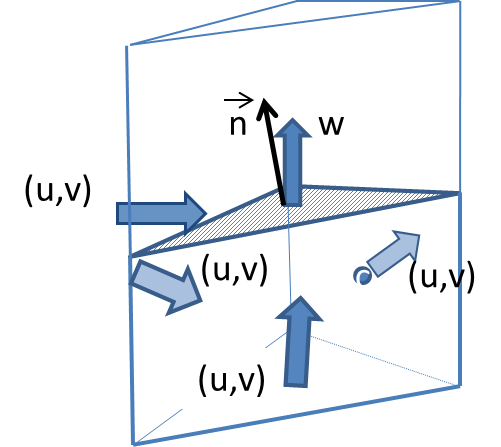
\includegraphics[scale=1.0]{image/vel_closure}
	\caption{First closure calculation on bottom prism. The horizontal velocities at the three vertical faces and the horzizontal component of velocity normal to the top face are shown and designated $(u,v)$. The vertical velocity $w$ is obtained from the 
	net flux. Movement of the S grid (typically a small fraction of a millimeter per time step) is not considered.}
	\label{fig:vel_close}
\end{figure}


\section{Discretization and data centering}
SELFE uses a triangular unstructured mesh in the horizontal direction and a bathymetry-conforming 
hybrid Z-S coordinate mesh \citep{Zhang08} in the vertical.

\subsection{Horizontal mesh}
The horizontal mesh is referred to as {\em unstructured} because the connectivity of the triangles 
is general and unconstrained. 
Unstructured grids incur some computational overhead because lists of neighbors must be tabulated as input and neighbors 
are not adjacent to one another in memory on the computer. The benefit, though, is that it is 
easy to represent complex shorelines with a fair amount of accuracy (see, for instance, Figure \ref{fig:hgrid}.

\begin{figure}
	\centering
		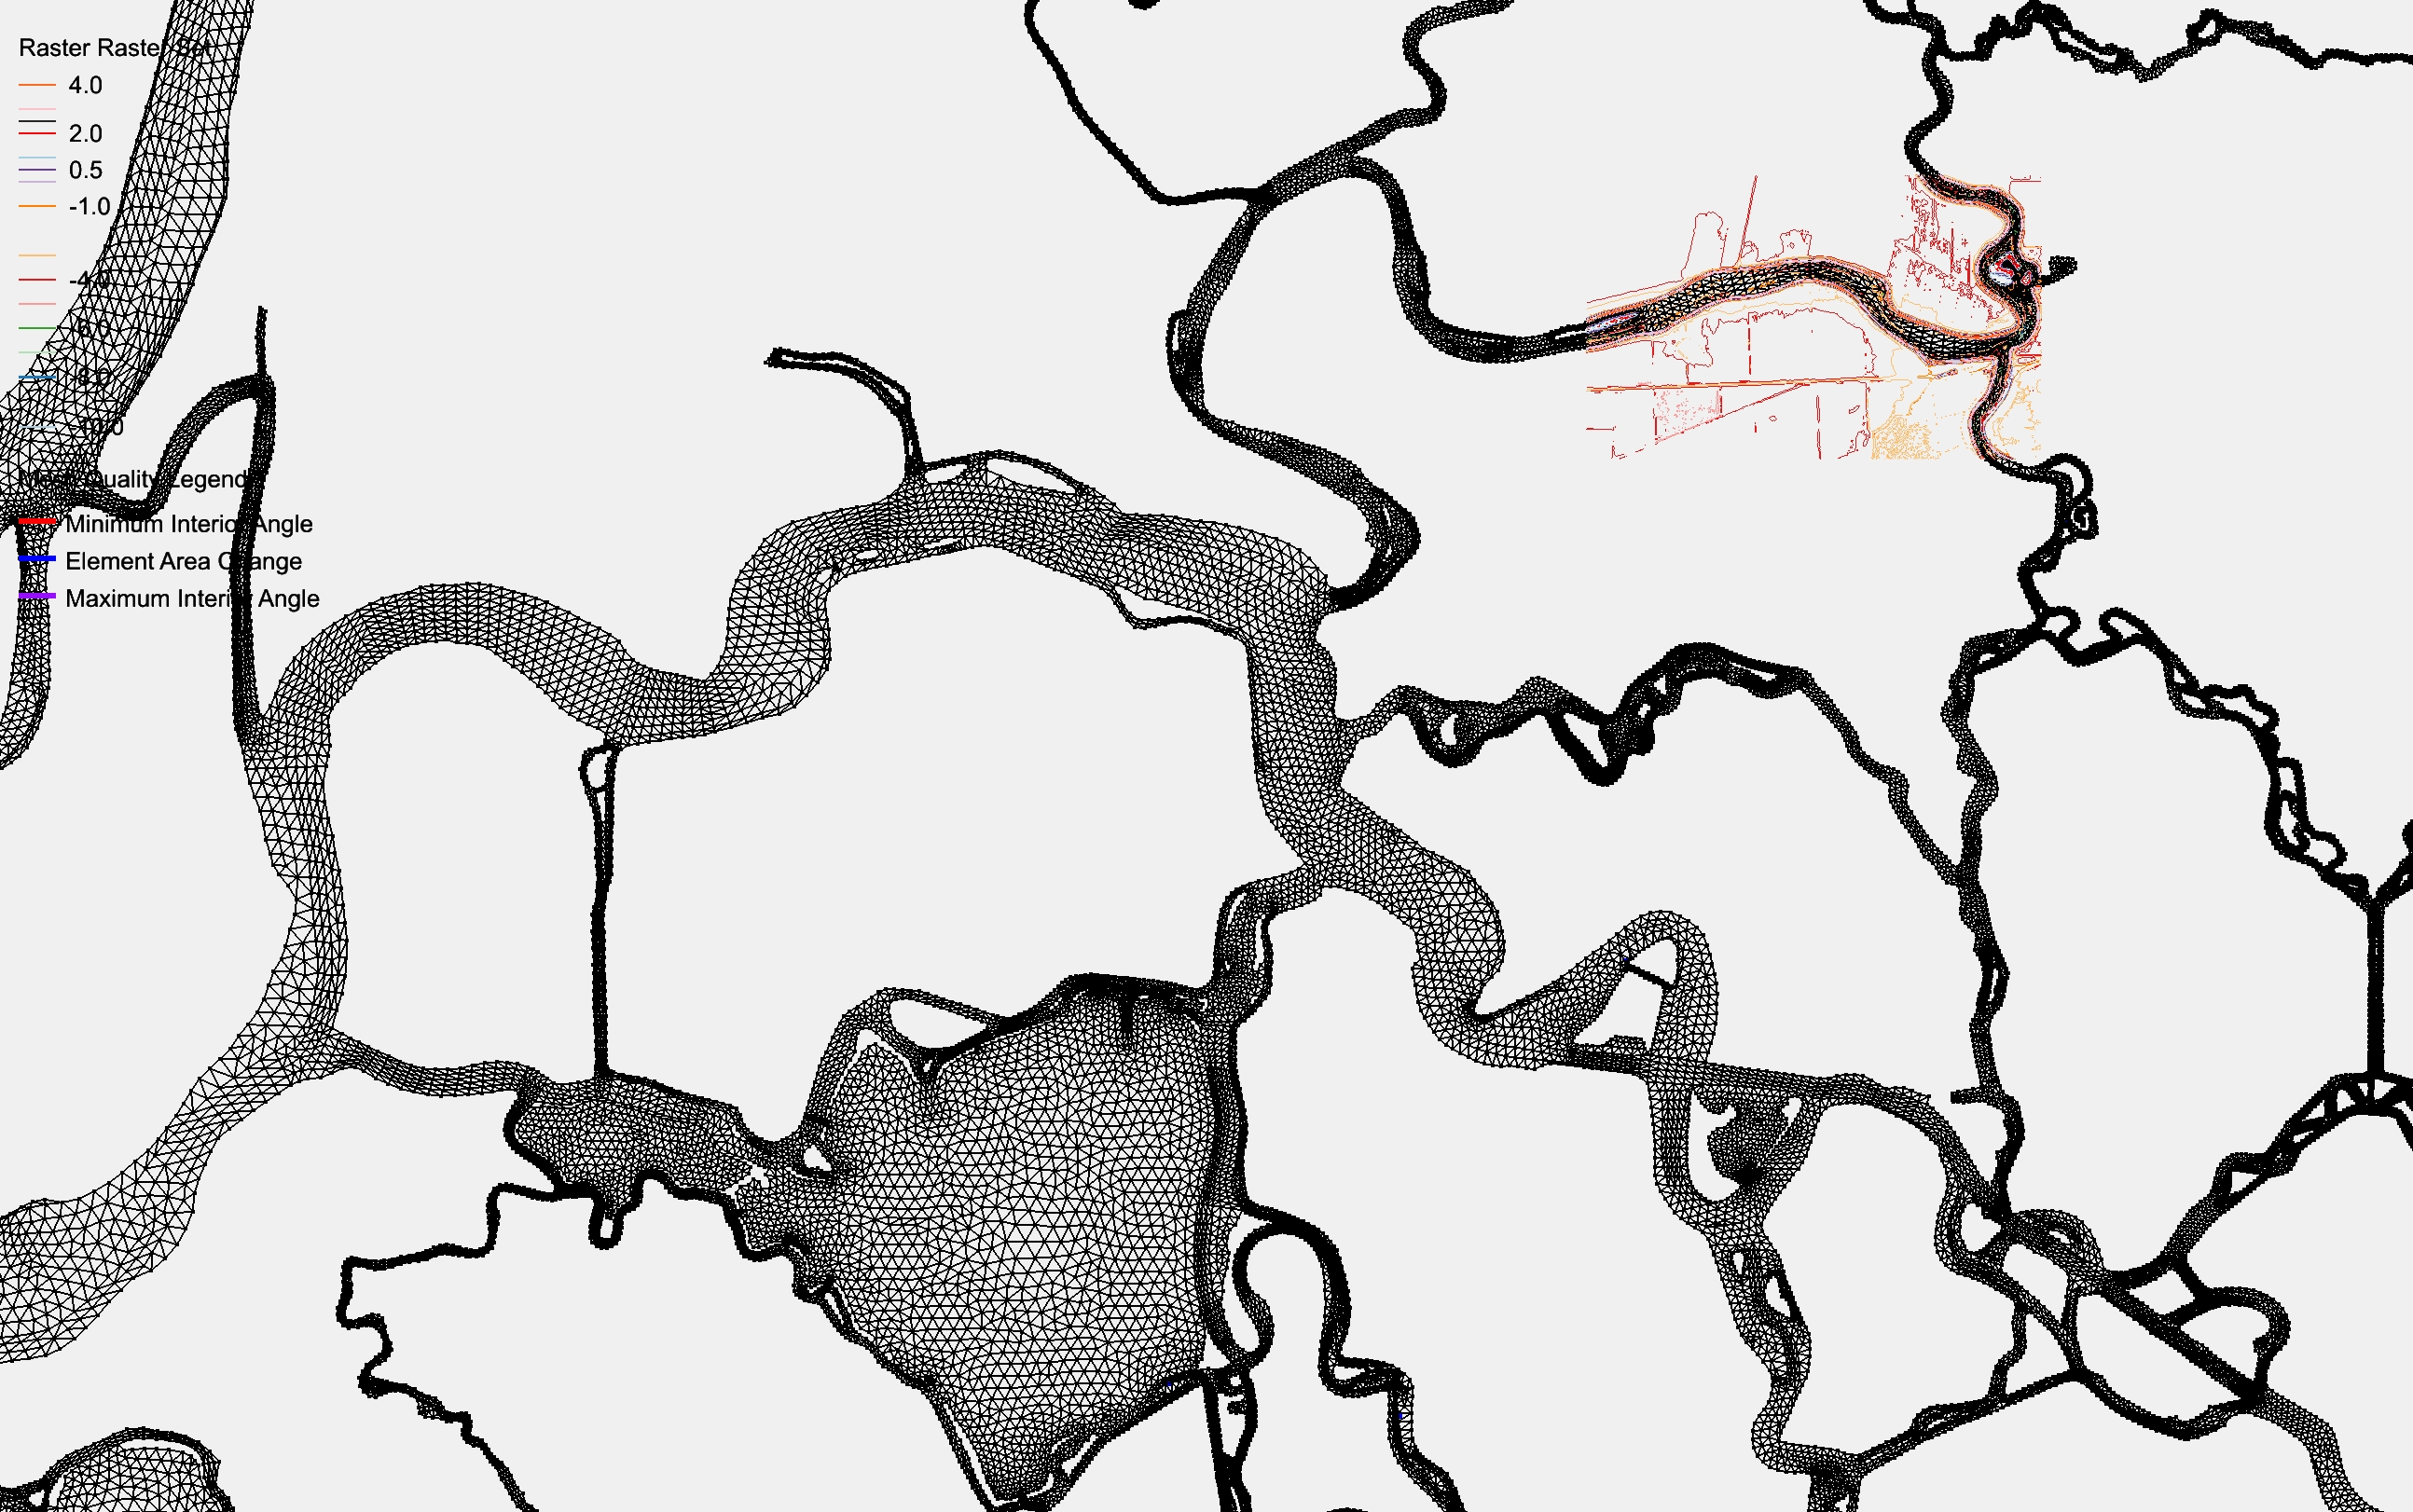
\includegraphics[width=\textwidth,clip,trim=3in 0in 2.5in 4.25in]{image/hgrid}
	\caption{Horizontal mesh near Franks Tract.}
	\label{fig:hgrid}
\end{figure}

\begin{figure}
	\centering
		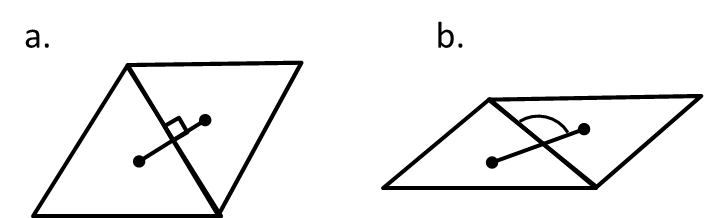
\includegraphics[scale=1.0]{image/ortho}
	\caption{a. Orothogonal triangular mesh. b. Non-orthogonal mesh with some skew.}
	\label{fig:ortho}
\end{figure}


One distinguishing characteristic of the horizontal mesh used in SELFE compared to 
semi-implicit models based on finite differences such as UnTRIM or SUNTANS is that the mesh is not 
required to be {\em orthogonal} (Figure \ref{fig:ortho}. An orthogonal mesh is one where the edges of the mesh are 
perpendicular to the line between the centers of the elements.  
For a triangular mesh, the orthogonality requirement leads to triangles that are nearly equilateral, 
a shape that enjoys some efficiency properties and nominally leads to higher accuracy even in SELFE. The
problem with orthogonal meshes is that they have traditionally
been expensive to generate, not only in terms of the dollar cost of the software involved 
(now lessened by software produced by \cite{Holleman13}) but also 
in terms of the tradeoffs they impose with other desirable properties such as conforming to the contours
at the foot of a slope at medium-low resolution. 



\begin{figure}
	\centering
		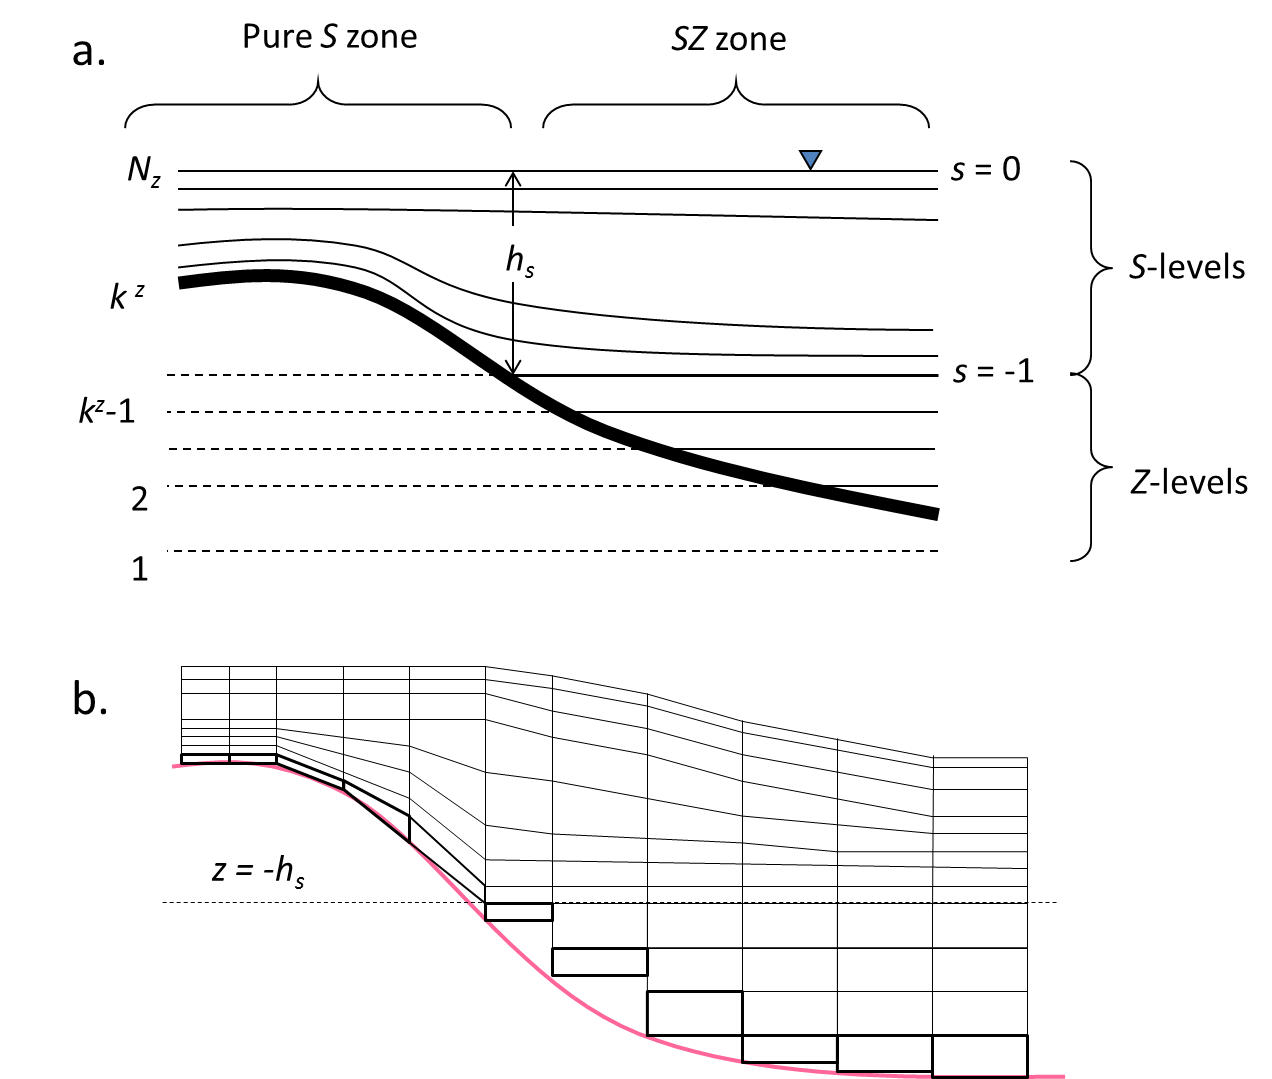
\includegraphics[scale=0.5]{image/vgrid}
	\caption{a. The hybrid coordinate system used in SELFE. S-coordinates are used above the threshold depth $h_s$,
	         while z (stairstepping) coordinates are used below. b. Vertical transect of an SZ mesh.}
	\label{fig:vgrid}
\end{figure}

Generating a good unstructured grid for SELFE requires some guidelines, and we'll elaborate on this in Section (\ref{sec-delta-mesh}). 

\subsection{Vertical mesh}
SELFE has a flexible meshing system in the vertical direction, allowing a hybrid
of Z layers below and S coordinates above as shown in Figure \ref{fig:vgrid}. 
The Z mesh has levels that are horizontal and is fixed 
at prescribed elevations, except for the partial level at the bed. This leads to 
a stairstep representation of the boundary as shown. The S coordinates \citep{Song94} are 
terrain following, with a constant number of levels between the bed (or uppermost z layer) and the free surface. 
The S grid parametrization allows the user to concentrate greater or less
density in the lower or upper boundary layers.  \gls{cmop} did extensive side-by-side 
testing of SELFE and ELCIRC, a Z-based model, and the terrain following mesh is one of the factors cited in the improved performance of SELFE.

As we shall describe in Section \ref{sec-delta-mesh}, we felt the Bay-Delta is generally shallow 
enough to avoid the $Z$ layers entirely.
The original purpose of the SZ hybrid was to avoid some of the pitfalls associated with topography conforming
meshes particularly on steep bathymetry in deep water, particularly so-called {\em hydrostatic inconsistency} and
the associated issues of inaccuracy in pressure calculations \citep{Shchepetkin05,Haney91}. Subsequent work on several basins, including the Columbia River, indicate that except in particularly steep, deep applications the pressure errors are secondary compared to the benefits of a terrain conforming mesh.

Although we are confident the pure-S approach is the best option available to us between S, Z and SZ,
we have also begun testing a vanishing quasi-sigma vertical coordinate system similar to that described by
\cite{Dukhovskoy09} in which layers disappear gradually in shallower water. Our implementation includes an
enhancement to avoid the stairstepping noted by  \cite{Dukhovskoy09}. This gridding system preserves the advantages
of bathymetry conforming coordinates while reducing pressure errors,
preserving stratification and eliminating some practical issues associated with 
over-resolution in shallow water. Such overcrowding of layers in shallow water almost always
occurs upstream if the deeper waters in the Bay are properly resolved).

Regardless of what vertical mesh option is chosen when running SELFE, the primary purpose of the mesh is to define the 
locations of the prisms in vertical space, which in the case of S coordinates changes over time with the evolution of
the water surface. This calculation is made once per time step; once that transformation is complete, the 
solver is based almost entirely on z coordinates.

\begin{figure}
	\centering
		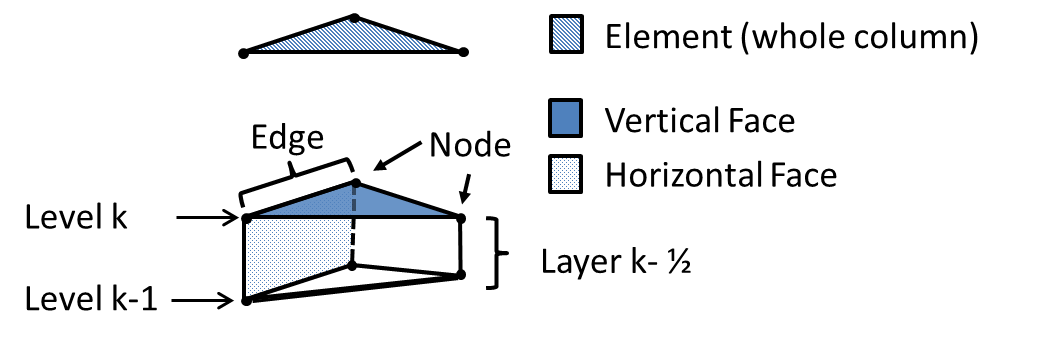
\includegraphics[scale=1.0]{image/prism}
	\caption{Nomenclature associated with a prism. Note that the term {\em element} is used for 
	the 2D horizontal component, and also for integrated quantities involving the entire water column. 
	.}
	\label{fig:prism}
\end{figure}


\subsection{Variables and mesh centerings}
Fig \ref{fig:prism} illustrates the nomenclature associated with the staggering scheme and variable locations used in SELFE. 
The surface elevation is defined at nodes, horizontal velocity at side (edges of an element) centers and whole levels (tops of prisms), tracers at prism centers (under upwind
or TVD transport schemes), and the vertical velocity at element centroids and whole levels. The staggering of variable enhances numerical stability \citep{Danilov13}. One difference to note between SELFE and other semi-implicit models
such as UnTRIM and SUNTANS is that SELFE calculates both components of velocity $(u,v)$ rather than a single
component normal to the edge. This is not relevant when calculating fluxes, but it avoids certain difficulties associated
with the Coriolis term. 

\section{Simulation steps and options}
\subsection{Outline of solution}
Details of the solution steps for the hydrostatic algorithm are given in the SELFE paper \citep{Zhang08}. 
Our goal here is only to sketch the algorithm, focusing attention on components that represent important
solver options. 

The time advance from step $n$ to step $n+1$ includes the following steps:

\begin{description}
\item[Momentum advection] The advection of momentum is handled using the \gls{elm} method. In an ELM, changes in advection are evaluated along flow paths, which means that characteristic paths have to be {\em backtracked}. 
\item[Evaluation of explicit terms] The momentum equation includes some terms that are implicit (the value
over the time step is estimated by a combination of the value at the old time $n$ and the new time $(n+1)$.
An example is friction.
Other terms, notably horizontal viscosity and Coriolis, are 
evaluated explicitly using only the value at time $n$. This 
step calculates the old time component of the implicit terms and
\item[Depth averaged mass and momentum] The depth-integrated mass and momentum equations are combined into
a single (2D) integral form and solved using the Finite Element Method. This step produces the new water surface
height $\eta^{(n+1)}$. 
\item[Horizontal velocity] is calculated algebraic from the momentum equation and new water surface algebraically
\item[Vertical closure] Vertical velocities are inferred from the horizontal ones and mass conservation.
\item[Transport] Salt and temperature are advanced using the velocity field just calculated. These will be used
in the hydrodynamics for density evaluation in the next time step
\item[Turbulence] closure is updated for use in the next time step (on a lagged basis)
\end{description}



\subsection{ELM options}
In SELFE, the momentum advection is {\em always} treated with ELM. The transport equation can be solved using ELM as well, although this is rarely done due to mass conservation issues associated with ELM. 

The ELM option treats the advection in an Eulerian-Lagrangian sense. For example, the total derivative of the velocity is approximated as:
\beq
  \frac{D u}{D t} \approx \frac{u^{n+1}-u^*}{\D t}
\eeq
where $u^n$ is the velocity at the new time step and $u^*$ is calculated 
by following a fictitious flow particle, starting at a pre-given point $\bs{x}$, backward in time and space 
(Figure \ref{fig:backtrack})
\begin{figure}
	\centering
		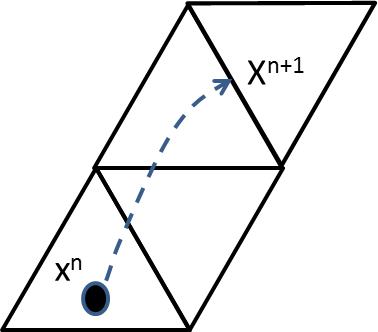
\includegraphics[scale=1.0]{image/backtrack}
	\caption{Backtracking of a fictitious particle is performed from the ending location at an edge center 
	(arrow) to the source (dot).}
	\label{fig:backtrack}
\end{figure}

The particle trajectory is determined by the characteristic equation, which moves the ficticious particle at the
the local (interpolated) velocity from the last time step.
\beq
  \frac{D \bs{x}}{D t}=\bs{u} \label{char}
\eeq

Variants of the method depend on how velocities are interpolated for purposes of backtracking and how 
quantities are interpolated at the foot of the characteristic path. 
 
In SELFE, the integration of (\ref{char}) is done using either a simpler backward Euler 
or 2nd-order Runge-Kutta scheme. To more closely follow the characteristic line, 
the integration time step is sub-divided into smaller steps.  After the foot of the characteristic line is found from (\ref{char}), $u^*$ is then interpolated using a scheme that is independent of 
the one used for backtracking. The order of interpolation function
used will determine if the ELM is diffusion (lower-order) or dispersion (higher-order) dominates the
error in the computation. In this project, the choice between lower-order interpolant was treated
as a calibration option. 


\subsection{Barotropic vs Baroclinic}
It is common, when speaking of the shallow water equations, to decompose the motion into
the barotropic and baroclinic modes. The barotropic mode is the most fundamental motion, 
and is associated with pressure gradients due to  variations in water surface height.
The baroclinic modes are induced by more complex vertical density structure
caused by salt (and temperature) differences.

In SELFE, the baroclinic and barotropic modes are toggled with a single parameter. They differ in that in Baroclinic mode, the contribution of temperature- and salinity-induced density differences is included in the momentum equations. In contrast, in Barotropic mode salt and temperature are (at most) considered passive tracers.
The turbulence closure is still calculated in 3D, but the suppression of turbulence due to stratification is not included.

One common usage pattern with SELFE is to use a sequence of barotropic-baroclinic model runs. The barotropic simulation is used in a preliminary simulation in order to calculate 3D boundary conditions (particulary the velocity) for the subsequent baroclinic analysis. Typically this is done with transport off or even, maximizing speed for the barotropic step and deliberately choosing diffusive model parameter combinations.

We believe the 3D mode can be used profitably for modeling the Delta alone with a boundary at Martinez,
particularly for studies that do not otherwise involve salt transport. The upstream part of the Delta is not stratified enough for baroclinicity to play an important role, and the cost savings of dropping salinity transport
is significant.

\subsection{Transport options}
There are three transport options available in SELFE:
\begin{enumerate}
\item \gls{elm}
\item First order upwind finite volume scheme
\item Higher accuracy \gls{tvd} finite volume scheme based on the scheme of \citet{Casulli05}
\end{enumerate}

We have already remarked that only the finite volume options are normally used. The first order and higher order TVD scheme can be hybridized on one mesh based on region or a depth-based switching criterion, and indeed the stringent \gls{cfl} time step restrictions of the TVD scheme more or less require this in shallow water. For this project, we used depth of 6m as the depth criterion and only used the TVD scheme below the confluence region.

\section{Wetting and drying}
 SELFE does not allow partial wetting and drying, and so the wetting and drying rule 
is based on full elements or edges. An element is wet if all
its 3 nodes are wet (based on the total depths there and a threshold minimum 
depth specified); otherwise it's dry. Based on this
information, a node is considered wet if and only if at least one of its surrounding
 elements is wet. Similarly, a side is 'wet'  if and only if at least 
one of its adjacent elements is wet. 

\subsection{Options}
There are two options for calculating wetting and drying at a new time step. The first consists of a simple sweep among all
nodes/sides/elements as described above. The second option is iterative starting from the shoreline position at the previous step.
The rule is applied at all shoreline nodes and adjacent elements and sides and the iteration is used to advance the shoreline from
one step to the next. At the end of iteration, a constant extrapolation scheme is used to 'project' the surface to the next
neighboring dry element. This option is designed for grids with adequate resolution so the inundation process can be tracked
accurately. For other grids, the first option should be used (as in the case of the current project).
\subsection{Implications for gridding}
\label{subsec-wet-dry-grid}
Because SELFE does not allow partial wetting and drying, the user must be careful not to grid the channel bottom too high such that
the entire channel is blocked from flow. In practice, it's best to at least use 2 nodes that are always wet in a channel, and use
extra nodes on either side to capture the wetting and drying process. However, if the other nodes are gridded too high, the side
elements may not be ever activated.

%add
\section{Hydraulic structures}
\label{sec-structures}
The term {\em hydraulic structures} refers to control structures such as tidally-operated gates, 
barriers, weirs and culverts as well as to coupled boundary conditions 
representing direct transfers of water from an outflow to an inflow boundary due to mechanisms like low head pumps. 
There are numerous gates and control structures in the San Francisco Bay-Delta. Here we describe the way structures are modeled and the formulas used to calculate flow through them. 

Hydraulic structures are represented in SCHISM as paired boundary condition (Figure \ref{fig:structmesh}). Flow is calculated based on head differences at two {\em reference nodes}, one on the nominal upstream and downstream sides of the structure (but not necessarily adjoining the structure). Once the flow is calculated, it is disaggregated as a homogenous flux boundary condition over the breadth of the structure. The boundaries are enforced using a relaxation formulation, which provides some natural ramping of flow when gates that are suddenly opened or closed. Transport is coupled between the side that is an outflow and the side that is an inflow.

\begin{figure}
	\centering
		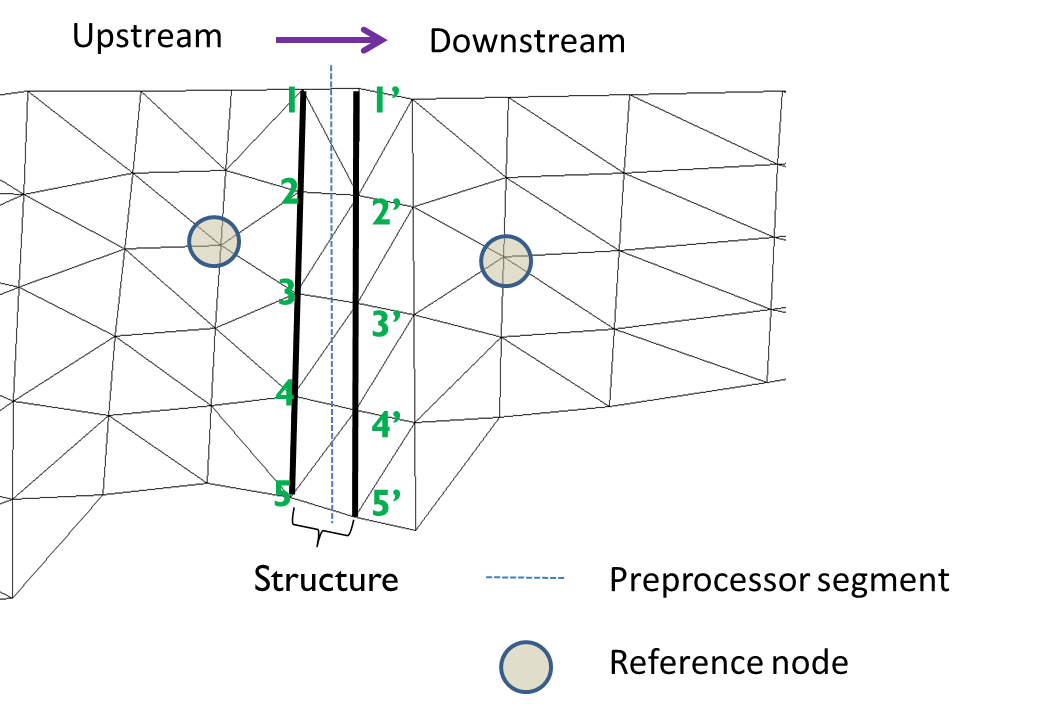
\includegraphics[scale=1]{image/struct}
	\caption{Hydraulic structure definition imposed on horizontal grid.}
	\label{fig:structmesh}
\end{figure}

A number of pre-defined flow structures are already in place covering all the cases we encountered in the Bay-Delta; with a little programming the system can easily be expanded to accommodate new structures.  
The structures we have already implemented are listed below. All of the structures admit control of key (indicated) parameters using time series. 

Structures can also be removed in SCHISM by adding 
an appropriate entry in a time series. When a structure is removed, the region between the paired boundaries reverts to the ordinary equations of motion -- ie, it is if the structure did not exist.

\subsection{Flow transfers}
\label{sec-transfer}
A flow transfer is a simple coupled boundary condition wherein a fixed flow $Q_s$ is stipulated. This flow
is imposed as an outflow boundary on one the paired boundaries and and inflow on the other. Constituent mass 
is conserved.

\begin{figure}
	\centering
		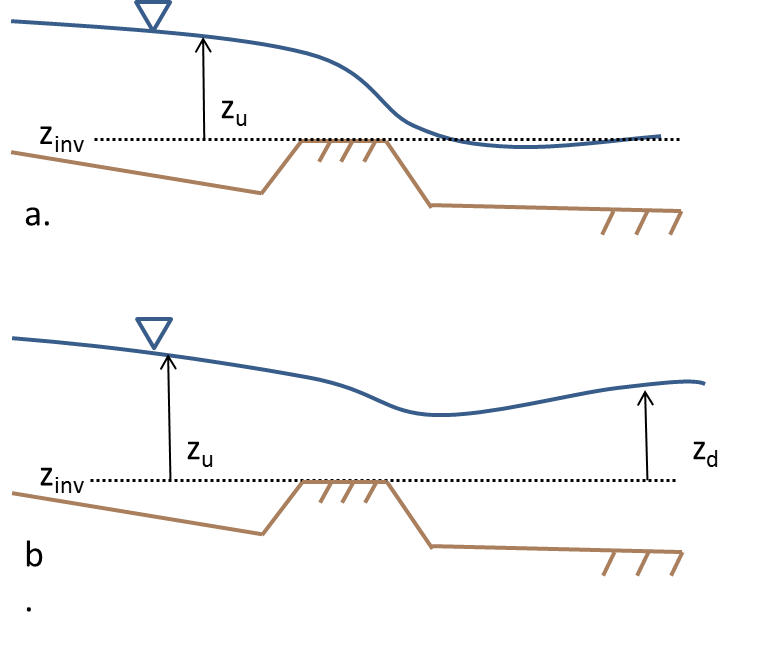
\includegraphics[scale=1]{image/weir}
	\caption{Free flowing (a) and submerged (b) weir flow cases.}
	\label{fig:weir}
\end{figure}

\subsection{Weirs}
A weir may be dry, submerged or free flowing (see Figure \ref{fig:weir}) depending on the position of the upstream
and downstream water surfaces $z_{u}$, $z_{d}$ compared to the weir invert elevation $z_{inv}$. Note that in the formulas
below, 

For the free flowing case:
$$
Q_s^f=\sgn{(z_{u} - z_{d})} C_{op} C_{f} A \sqrt{2g H}
$$
where 
\begin{align*}
&Q_s^f  &\text{free flow flow through structure (cms)} &\\
&\sgn        &\text{sign function (to induce up/downstream directionality)}  &\\
&z_u         &\text{upstream reference elevation  (m)}  &\\
&z_d         &\text{downstream reference elevation (m)}  &\\
&z_{inv}     &\text{invert elevation of the weir (m)}  &\\
&H = \max(z_u,z_d) - z_{inv}  &\text{is the energy head above the weir} &\\
&A                            &\text{area of flow (m\textsuperscript{2}) }&\\
&C_op               &\text{(directionally varying) operating coefficient (unitless)} &\\
&C_f                &\text{flow/gate coefficient (unitless)}  &\\
&g                  & \text{gravity (m/s\textsuperscript{2})} & \\
\end{align*}
For commentary on coefficients, see \cite{Rantz82}. Note that in the formulation above, the $\sqrt{2g}$
term has been kept separate and the area calculation uses water surface height. 
Furthermore, note that $z_u$ and $z_d$ are pre-assigned upstream and downstream orientations,
whereas $H$ is the energy head in the direction that is upstream of the weir in terms of actual flow.

The submerged case is derived from the free flowing case using the correction given by \citet{Villemonte47}:
\begin{align*}
Q_s^s = Q_s^f(1 - S^{1.5})^{0.385} \\
S = \frac{\min(z_u,z_d) - z_{inv}}{\max(z_u,z_d) - z_{inv}}
\end{align*}
in terms of the {\em submergence ratio} $S$.

If both sides are dry, of course $Q_s=0$ for the structure. Note that this refers to being dry with respect to the invert elevation.
The nodes may not go dry in the ordinary sense with respect to the bed -- this is the same restriction as at other SCHISM boundaries. 

\subsection{Radial gates} 
\label{sec:radial}
A radial gate is parametrized as shown in Figure \ref{fig:radial}, although at the moment we have ignored the kinetic 
energy component of upstream head (so that $H_1 = y_1$). For the case where the radial gate is completely out
of the water or the tailwater elevation is not sufficiently high to affect the upstream (submergence ratio described in the previous
section is less than $S_p=0.66$),
the gate reverts to a modified weir equation described momentarily. For the case where the radial gate is completely submerged 
(submergence ratio greater than $S_f=0.80$),
the gate is treated as an orifice as given in Section \ref{sec-orifice}.

            %diff = max_elev - min_elev
            %coef_matching_factor = sqrt(1.d0/(1.d0-PART_SUBMERGE))
            %flow = signed_coef*area*sqrt2g*sqrt(diff)
            %! now weigh the two so that the flow makes a linear transition
            %subfrac = (submerge_ratio-PART_SUBMERGE)/(FULL_SUBMERGE - PART_SUBMERGE)
            %flow = ((1.d0 - subfrac)*coef_matching_factor + subfrac)*flow
For free flow:
$$
Q_s^f = \sgn{(z_{u} - z_{d})} C_{op} C_{f} A \sqrt{2g H}
$$
and for partially submerged flow ($S_p < S \le S_f$):
$$
Q_s^p = \sgn{(z_{u} - z_{d})} C_{op} C_{f} A \sqrt{2g \left|\D z\right|}[(1-\hat{S})m+\hat{S}]
$$
where
\begin{align*}
&\hat{S}=\frac{S-S_p}{S_f-S_p} & \text{is the submergence fraction} \\
&m = \sqrt{\frac{1}{1-S_p}} & \text{is a coefficient matching factor to create a smooth transition}. \\
\end{align*}

For fully submerged flow $S>S_f$, the orifice equation is used. This is equivalent to the submerged equation with
$\hat{S}=1$.


\begin{figure}
	\centering
		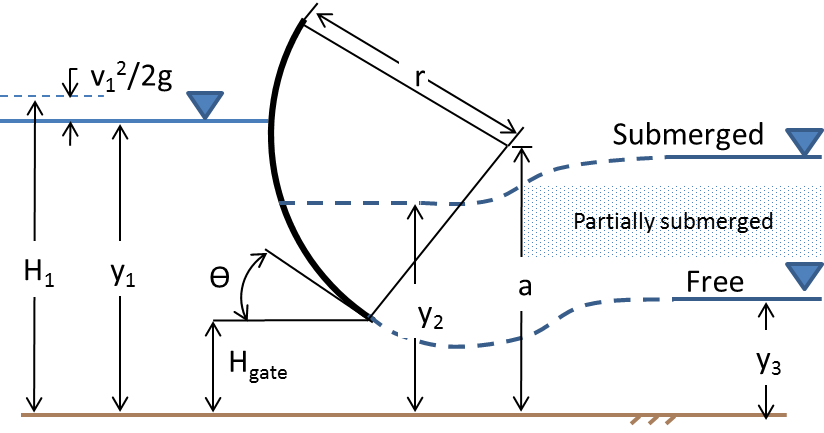
\includegraphics[scale=1]{image/radial_gate}
	\caption{Radial gate.}
	\label{fig:radial}
\end{figure}

\subsection{Radial gates with linear coefficient} 
This is an alternative radial gate formula modified from a suggestion by Tony Wahl of the USBR (personal communication) 
that was incorporated because it matches Clifton Court well. 
The rating formula is a little simpler, but the flow coefficient is a linear function of gate height:

$$
Q_s = \sgn{(z_{u} - z_{d})} C_{op} C_{f} A \sqrt{2g \left|\D z\right|}
$$
where
$$C_f = d + sR$$
is the gate coefficient linearly dependent on the ratio of gate opening to upstream head:
$$R = \min(\frac{H_{gate}}{H_1},1.0)$$
with constant and linear parameters $d$ and $s$ respectively.
Some special cases surround the term $A$, given that the top of the radial gate
may be dry or submerged.

\subsection{Orifice}
\label{sec-orifice}
The orifice option is used to model a sluice gate or flashboard or other devices that  
presents a (rectangular) apertures to flow. Flow in this case is given by:

$$
Q_{s} = \sgn{(z_{u} - z_{d})} C_{op} C_{f} A \sqrt{2g \left|\D z \right|}
$$

Some special cases surround the term $A$, given that the orifice may be dry, partially submerged or completely
submerged. Typically, the orifice equation is most useful when flow is fully submerged.

\subsection{Culverts}
A culvert is currently modeled as a circular orifice. In other words, it is the same as the orifice case
but with a different formula for $A$. This treatment neglects some of the nuances of head and tailwater control 
as described by \cite{Bodhaine68}



\section{Mass sources and sinks}
\label{sec-source}
Assuming that the extra momentum from the sources and sinks is negligible, 
we accommodate sources through the by adding them to the continuity equation (\ref{cont1}):
\beq
  \eta_t+\nabla \cdot \int_{-h}^\eta \bs{u}  = \sum_m s_m(t)\hat{S}(\bs{x}-\bs{x}_m) \label{cont2}
\eeq
where $s_m$ is the discharge, and $\hat{S}$ is a Dirac delta function defined at a series of points $\bs{x}_m$ (in the model we
assume these are located at element centroids). Note that the transport equation (\ref{tr1}) already accounts for the sources and sinks in the term $\hat{Q}$.


\section{Model-specific sources of error/uncertainty}
  \subsection{Mass conservation}
    SELFE does not explicitly enforce volume conservation (through the continuity equation), 
		due to the Galerkin \gls{fem} used in the solver. Mass
conservation for tracers is however enforced with the upwind/TVD schemes, as a consistent treatment is used for the 3D continuity
equation (\ref{3Dcon}) and the transport fluxes.
	\subsection{Vertical closure for flow over topography}
    This error is related to the volume conservation error shown above. The horizontal divergence drives the vertical velocity, which is calculated starting from the bottom b.c. and progressing upward. The mismatch between the calculated vertical
velocity at the surface and the b.c. there is the closure error. The error can be large when the bottom slope is large (e.g., Golden
Gate). Judicious gridding and choice of vertical grid can alleviate this error somewhat. 

   Note that even if the volume is perfectly conserved, the vertical velocity may still become too large at the surface due to other
reasons as explained in Wolfram and Fringer (2013).
	\subsection{Shallow water and friction}
    The use of a large bottom friction in shallow areas in SELFE3D can lead to parasitic oscillations due to spurious wetting and
drying. This is particularly the case when the channel is narrow and under-resolved. In this case, the 3D model tends to generate
large vertical shear as the flow is being blocked. Note that SELFE2D does not have this issue as a 2D model cannot allow vertical
shear. 
    Obviously this has implication for gridding. A simple work-around is to ramp the friction down in the shallow areas to alleviate
the shear. This approach has worked reasonably well for Bay-Delta domain. 
	\subsection{Diffusion-dispersion characteristics}
  SELFE has a myriad of schemes inside. Some schemes are more diffusive than others. An example is the interpolation schemes used in
ELM. Another example is the scheme used to convert side-based velocity from node-based velocity. This can be done using a simple
weighted averaging scheme which is more diffusive, or using the linear conforming or non-conforming shape function inside each
surrounding element before averaging. The latter is more dispersive, and requires a 5-point Shapiro filter to filter out spurious
sub-grid modes. 

\chapter{Bay-Delta SELFE Application}
\section{Application introduction}
Thus far we have described the SELFE model in the sense that it is an algorithm or piece of software,
including modifications (hydraulic structures and mass sources) that we made as part of the current project.
In this section we describe the {\em model application}; viz, the model configuration including 
the extent of the domain, mesh, initial and boundary conditions needed to drive the model. 

\section{Datum and units}
For spatial data, the project projection is NAD 1983 UTM Zone 10N based on North American Datum 1983.
The vertical datum is NAVD88 (North American Vertical Datum 1988), and this is the datum used in the 
model to partition total depth into unperturbed bathymetric depth and free surface elevation (see 
Figure \ref{fig:depths}).

The model calibration is configured in SI units, which are assumed in SELFE. Results are also 
given in SI units but English units are indicated on many of the plots.

The unit of salinity used inside SELFE is the \gls{psu} as defined by the 
Practical Salinity Scale of 1978 (PSS-78). While standard in oceanography, 
the PSU is sometimes an unfamiliar unit to Delta modelers and managers. 
It is virtually identical to parts per thousand (ppt) of salt -- 
a somewhat more familiar unit used to define some of the Delta water quality standards.
For instance, X2 happens where bottom salinity is 2 psu.

The more common way of observing salinity in the Delta is through the surrogate \gls{ec}.
In fact, when agencies (USGS and NOAA) report salinity in PSU (rather than ionic concentrations
such as chlorides), the practical salinity is back-calculated from EC.
Given the importance and familiarity of conductivity, in this document we
 often include conductivity in plots on a second axis. 
Conductivity is give in $\mu$Siemens/cm at $25\,^{\circ}\mathrm{C}$, which 
is an SI unit equivalent to $\mu$mmhos/cm. The (nonlinear) relationship between EC and
salinity is the one quoted by \cite{suits2002} including the Hill correction in the dilute range 
below 2.0 psu but not including corrections for agricultural salt. This relationship is shown in
Figure \ref{fig:ec_psu}, which also demonstrates the smallness of the Hill correction.   

\begin{figure}
	\centering
		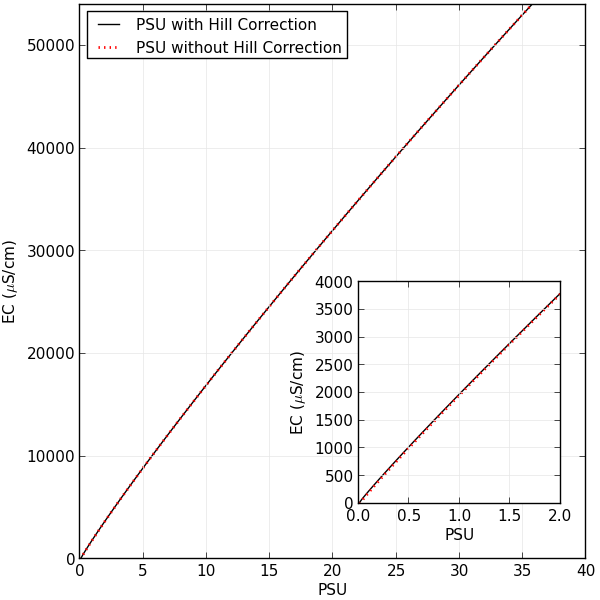
\includegraphics[scale=1]{image/ec_psu}
	\caption{Relationship between Practical Salinity Units (psu) and Conductivity 
	  ($\mu$S/cm at $25\,^{\circ}\mathrm{C}$) for the full range (main plot) and low (inset) salinity.}
	\label{fig:ec_psu}
\end{figure}

\section{Mesh}
\label{sec-delta-mesh}
The full Bay-Delta mesh is shown in figure *** and four example sections of the horizontal mesh are shown in Figure***. 
The mesh presented in this calibration comprises ~210000 triangles and ~130000 nodes. 

The Bay-Delta Mesh was constructed using the Aquaveo SMS generic software package, in which the user first specifies a 
skeleton {\em mesh map} comprised of discretized polygons (which can come from contours, 
GIS polyline coverages or simply be hand-drawn), each of which is then filled using 
one of several automatic meshing algorithms. Local resolution is controlled by
the spacing between vertices in the line segments of the mesh map as well as control points. Dense maps representing 
mesh size functions can also be provided by the user, but this option was not utilized in the present project.

Two generation algorithms are employed. An advancing front algorithm ("paving", figure **) is used for 
larger, well-resolved regions and also in some side embayments. Advancing front methods work particularly well in areas
like the coastal part of the model where the body of the polygon to be filled is large in every dimension compared
to the discretization length. Coons patches ("patching", figure **) are used in channelized areas, including the main part of Delta channels and the internal channels in some bays and open water bodies. The advancing front method produces more optimally shaped (ie, equilateral) triangles but is difficult to control in tight areas so that it conforms to bathymetry well. The
Coons patch looks more like a curvilinear grid and can follow and resolve sinuous channels or contours. Figure *** compares
the result of a Coons patch with paving for a narrow channel.

The SELFE Bay-Delta mesh resolution varies from approximately 1km in the ocean, 100-400m in the Bay and down to 15-60m in Delta
channels, with the smalles element size of ~2.5m found near some narrow channels of Middle River. The mesh sizing was chosen
\begin{itemize}
	\item to resolve bathymetric features and the deep sections of major channels (including internal channels in bays)
	\item to resolve lateral and vertical variation in velocity, as determined by sensitivity studies on velocity and
	salinity transport
	\item to emphasize regions of policy importance or that have a greater effect on global accuracy
	\item to take good advantage of SELFE's ability to handle anisotropy and non-orthogonality robustly in less resolved areas (our
experience suggests that the model can effectively handle skew elements with skewness up to 20).
	\item to realistically introduce wetting and drying while keeping always-wet main channels open to flow
	\item with consideration given to time step (CFL) implications, emphasizing regions that could be refined without introducing 
	excessive numerical diffusion (in ELM) or subcycling and performance issues (transport, particularly with the TVD algorithm).
\end{itemize}

These criteria were supported by numerous prototype meshes and informal sensitivity studies, 
particularly in the Carquinez Strait and Suisun Marsh. Although we are aware of automata 
that may support many of these criteria (most notably \cite{Persson2004,Persson05}, and
on simple reaches these methods produce very beautiful meshes. However the resulting loss functions
for mesh size are complex and implementing them will require specialty additions to software. 
In contrast, most general purpose meshing software is overly dedicated to either 1) measures of local accuracy
or 2) boundary curvature (ie, the shores, not the contours that delineate the deep part of the channel).
 
Modeling narrow channels and openings efficiently requires some care with SELFE, because the free surface (stage)
is modeled at mesh nodes and care must be taken that the wetting and drying rules 
(see Section \ref{subsec-wet-dry-grid}) do not engage prematurely and choke off the channel at low tide. This is not much of a restriction in larger, well-resolved channels such as the Sacramento *** (figure ***) where less than *** of the channel area
and most of the bathymetric uncertainty is concentrated on the levee slope (see \citet{Wang12}). For narrower channels
that are not resolved 5-6 elements across such as the Mokelumne, the meshing strategy shown in Figure *** is used whereby the levee slope is either ignored (left bank) or nodes are carefully placed to resolve the bank (right).


The overall shallowness of the Bay-Delta system allows us to use the terrain-following coordinate system ($S$) alone without $Z$
layers, thus avoiding a staircase grid everywhere. We set a modest value for the stretching constant ($\theta_f=1$) and chose ($\theta_b=0.5$) so more resolution is placed near the surface  than near the bottom. The transition depth at which $S$
reverts back to traditional $\sigma$ coordinate system was set at $h_c=10m$, and so only the deeper channels are discretized using
$S$, whereas vast shallow areas use $\sigma$. After some sensitivity tests, the total number of levels was fixed at 23.

One outside commentator were curious why we did not use hybrid coordinates to avoid over-resolving the upper estuary. 
The issue can be seen in Figure \ref{fig:vgrid}. The number of S levels has to be set to 
adequately revolve the deepest water. In our case, this is the 
Golden Gate at 100m and the resulting number of layers is 23. This is clearly more 
than necessary in the channels upstream which might be 4-10m deep. Although this represents
a potential inefficiency, experience by SELFE users on other basins apparently indicates two reasons not to use
SZ hybrid grids unless absolutely necessary: reduced accurate from the stairstepping Z grid and
a potential small numerical boundary layer caused by the transition from S to Z. We are currently 
developing a mesh based on pseudo-sigma coordinates similar to those used by \citet{Dukhovskoy09} but without the
stairstep noted by \cite{Siddorn13}. A pseudo-sigma coordinate system is terrain-following like an S-grid
but allows S levels to vanish in shallower water. The primary advantage to pseudo-sigma coordinates, as with SZ,
is to flatten the levels in steep topography and improve pressure calculations. However, it can be configured in
a way that that has the ancillary benefit of reducing vertical resolution in upstream areas.


\section{Bathymetry} 
SELFE requires bathymetry data at every node in the mesh. Bathymetry preparation for multidimensional modeling is described in \cite{Wang12}. 

Our bathymetry integrates elevation data from previous USGS maps, single and multibeam data collections into a set of consistent 10m and 2m elevation DEMs. 
The data used in calibration is identical to the Version 2 release of this bathymetry except that here 
we have incorporated recent improvements near the CVP intake and South Delta, 
and some additions in the North Sacramento where we extended the bathymetry in response to boundary reflection. Artificial deepening was performed at a small number of nodes 
(fewer than 0.1\%) to reinforce the connectivity or conveyance of the channels in areas where photography indicates error in the 
DEM or where underresolved shallow undulations were detrimental to model performance.




\subsection{Volumetric and face optimization}

Once the mesh is fixed, the bathymetry is assigned to the nodes of the model
 in such a way as to ensure fidelity not only to the point value 
of the bathymetry at nodes (which are where SELFE stores  bathymetry) 
but also to the volume of the elements and to the area of the 2D vertical faces 
along the edges of the mesh. 

This volume and area matching is performed by solving a weighted, regularized 
least squares problem that penalizes differences between the SELFE representation of the bathymetry
(which amount to a TIN) and the result of much denser Gaussian integration over the elements and sides.
All samples from the DEMs are taken using bilinear interpolation from the best quality DEM available for the 
requested point.

\begin{align}
   &\Min_{z_n, n=1,N_p}
   \begin{aligned}[t]
      &\sum_{e=1}^{N_e} \frac{1}{A_e}(V_e - V_e^q)^2 + \beta_s \sum_{s=1}^{N_s} \frac{1}{l_s}(A_s-A_s^q)^2 \\
      & + \alpha_n \sum_{n=1}^{N_p} (z_n-z_n^{0})^2 + \alpha_s \sum_{s \in \Gamma_{l}} (\Delta z)_s^2
   \end{aligned} \notag \\
\end{align}

where:
\begin{align*}
&N_e, N_s, N_p  &\text{number of elements, sides, nodes} &\\
&\Gamma_{l}  &\text{set of all sides on land boundaries} &\\
&V_e            &\text{volume of element (SELFE)} &\\
&V_e^q          &\text{volume of element (quadrature)} &\\
&A_e            &\text{horizontal area of element (SELFE)} &\\
&A_s            &\text{vertical area of side (SELFE)} &\\
&A_s^q          &\text{vertical area of side (quadrature)} &\\
&l_s            &\text{length of side} &\\
&z_n            &\text{elevation assignment} &\\
&z_{n}^{0}    &\text{original elevation from DEM } &\\
&\Delta z_n     &\text{(undivided) difference in elevation along side}  &\\
&\beta_s        &\text{weight of area}  &\\
&\alpha_n, \alpha_s  &\text{regularization weights} \\&
\end{align*}

The first two terms of the loss function penalize deviations in volume and area. The last two are
small Tikhonov-like regularization terms that penalize deviations from
the original point values interpolated from the DEM and also penalizing sharp fluctuations 
along land boundaries. The loss function weighs elements equally so it is 
not quite the discretization of a continuous problem.

The result of this optimization process is a small vertical adjustment to the depth assignments at nodes, which is where SELFE
stores bathymetry. Figure \ref{fig:optimization} gives some indications to what extent optimization can make up for volumetric error. The difference in element-averaged bed depth (based on a reference surface of ***) 
is shown for the SELFE representation shape functions and 14-point quadrature. 
Four cases are shown -- two different meshes, each with and without quadrature. 
Mesh 57 was a manual reworking of mesh 50,  specifically aimed at delineating the foot and top of slopes along the Sacramento.  
The figure clearly shows that the optimization can reduce error but the improvement is not a substitute for good horizontal placement of the nodes.
 
\begin{figure}
	\centering
		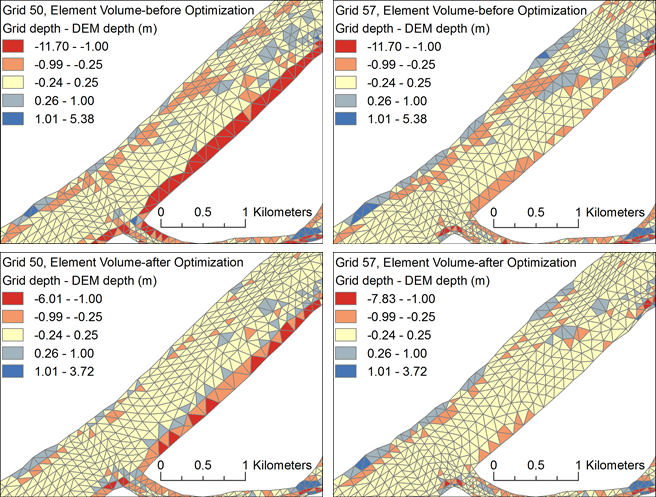
\includegraphics[scale=1.00]{image/optimization}
	\caption{Volume discrepancies for two versions of the mesh, before (top) and after (bottom) volumetric optimization.}
	\label{fig:optimization}
\end{figure}


We have verified that this bathymetry cleanup produces better flows at most sites. 
One unanticipated benefit of the optimization is the suppression of
 unrealistic undulations on the shore prevents erratic wetting and drying. The difference in the shoreline is shown 
in Figure ***, which compares a shore segment before and after optimization. 

The optimization does relinquish 
some of the control over elevations that can come from, say, very close digitizing along contours. 
This control can be an issue when planning for adaptive aspects of the algorithm that 
depend on depth thresholds, such as the switching between TVD and upwind transport schemes. In such cases, 
one usually wants to mesh just above or below the TVD threshold. 




\subsection{Deepening near boundaries}
SELFE does not restrict the value of inflows in any way (zero or withdrawal is fine), but it does not allow boundaries to become
dry. This modeling requirement is not at odds with our desire to extend the mesh up the major rivers beyond the region of tidal influence, but
it does raise some practical problems with initial conditions and boundary conditions at startup. If we na\"{\i}vely
initialize using a water surface gradient based on interpolation or steady state principles, the initial transient can 
behave like a flood wave. What we have found is easier is to use a flat water surface at a reasonable high tide value and impose
a maximum bed elevation near the boundary that will be wet at this level (Figure ***). Our experiments indicate no appreciable
sensitivity to this treatment.


\section{Initial conditions}
SELFE requires an initial condition for the entire model state, including velocity, water levels and salinity. Because the main
tidal hydrodynamic information propagates very quickly from the boundaries to the rest of the system, the domain has only a brief
memory (2-3 tide cycles) of velocity and surface elevation initial conditions. As long as the salinity field is reasonable (to
stabilize baroclinic movements), the main criteria in selecting elevation and velocity initial conditions are practical ones: to
minimize startup transients and maximize compatibility with boundary conditions. These goals are easier to achieve with very simple
flow fields; hence we cold start these variables from a velocity of zero everywhere and an elevation of 0.96m NAVD 
which is a medium-high tidal water level. To increase compatibility between the velocity and boundary conditions (which, when careless introduced into a non-diffusive model often result in mini-tsunamis or water hammers), the elevation and velocity
boundary conditions are ramped up linearly from zero over a few days. 

The system memory for salinity is much longer -- at least several months -- and it is helpful if the salinity initial condition roughly captures field conditions particularly in the Bay. The salinity initial condition was generated regionally:
\begin{itemize}
	\item Ocean: A scalar value of 33.5 psu at all depths,  which is typical of the shelf region at modest depth \citep{Dever94}.
	\item Bay and Suisun: From the South Bay to the confluence the model is initialized using \gls{ctd} casts from USGS water quality cruises, interpolating linearly longitudinally between stations and extrapolating radially as a constant from the centerline of the cruise.
	\item Delta: A scalar constant value of 0.1 psu (213 $\mu$S/cm EC) throughout the Delta. This value is typical for the north Delta but probably relatively fresh for the South Delta.
\end{itemize}

To minimize the influence of salinity initial conditions from our March 12, 2009 calibration simulation start date, we do not generate salinity skill statistics before June 1, 2009 for the Delta and May 1, 2009 for the Bay.

Some ongoing effort is underway to minimize spinup time by briefly (March 12-15 in this case) assimilating data from observation stations in the Delta through nudging (Newtonian Relaxation). SELFE has the ability to assimilate data in this manner, but time did not allow us to complete the data preparation work in time for this document. 

\section{Ocean boundary}
  \label{ocean-boundary}

\subsection{Boundary placement}
In order to use our model for processes that extend to the ocean (salt intrusion under sea level rise, full life cycle salmon modeling) the boundary of the model must be far enough offshore so that the dynamics of the domain do not impact the boundary. The ocean boundary of the Bay-SELFE model lies on a roughly 46km radius arc from the Golden Gate, extending from Point Reyes to the Farallon Islands and south just past Half Moon Bay (Figure ***). This shape and placement is similar to the boundary described by \citet{Chua2011} in their  model of the San Francisco Bay using SUNTANS. An alternative is described by \citet{MacWilliams08,MacWilliams09} in their UnTRIM application; they use a straight boundary oriented along isobaths in the alongshore direction.
%
Our placement of the boundary attempts to reconcile these conflicting factors:
\begin{itemize}
\item The size of the likely temperature, fresh water or sediment plume.
\item The orientation of bathymetry and likely propagation directions of tidal constituents
\item Structure of currents
\item The model coupling to ROMS in the SESAME project
\item Locations of available boundary tidal information.
\end{itemize}

The primary consideration was containing the freshwater jet and plume from the Bay on ebb tide, which we felt was easier to do with the semi-circular boundary configuration. Figure \ref{fig:plume2} shows a snap shot of the sediment plume exiting from the San Francisco Bay (**permission). \citet{Hurst08} have described evidence of plume fronts as far as 122.66\textdegree W (indicated***), or roughly 20km from the Golden Gate.
\citet{Carlson74} analyzed aerial photos of sediment plumes in the early 1970s and observed plumes approximately 30km from the Golden Gate during high outflow periods in 1970 and 8km during lower, more typical, outflow conditions. Using satellite imagery supported by in situ measurements, \cite{Ruhl01} measured sediment plumes at 15km from the Golden Gate based on suspended sediment, although the pertinent figures in that paper suggest that above-ambient sediment concentrations farther (perhaps 30km). 

At 45-46km from the Golden Gate, our domain should contain the fresh water plume under all but the most exceptional conditions. This
distance is also a maximum practical size of the domain. [b.c. is the main concer as you pointed out] 
 Locating the ocean boundary entirely on the shelf is preferable to partially extending it to the continental slope.
This is particularly the case off the California coast -- the summary by \citet{Noble2001} indicates a significantly
different tide and current pattern on the shelf and slope. Nuanced differences such as these would not be reproducible without data assimilation, very detailed boundary conditions and improved atmospheric data, none of which is possible to provide in a hypothetical planning context 
and which are unlikely to improve global accuracy in areas of greatest policy interest in the interior Delta.

Although we selected the arc as our boundary, the orientation of the bathymetry and tidal propagation suggests some important
hydrodynamic features vary most simply along the straighter isobaths that run in the alongshore direction of the greater Califonia
coastline. Figure *** shows contours of local bathymetry and makes this direction clear; Figure *** shows predicted isocontours of
amplitude and phase of the largest semi-diurnal (M2) and diurnal (K1) tidal constituents along the near coast according to WEBTIDE,
 a modeling product that uses data assimilation and ocean dynamics to map tidal constituents. Inasmuch as a trend is evident, it follows the alongshore direction. We had some difficulty validating these spatial trends of constituents in field data, in part because of the local character of some of the records such as Bolinas Bay. 

The orientation of currents is much less predictable. Large scale trends in mean currents tend to vary depending on season and whether upwelling is occuring.  Patterns observed using tidally averaged 6km HF Radar (***) also indicate a number of local current patterns offshore forced by prevailing winds and bathymetry such as the promontory of the Point Reyes peninsula. Given the small magnitude and peculiarities of velocities offshore and our inability to reproduce them in a planning setting, we use the alongshore variation in tidal constituents in preparing our surface boundary data, not in the orientation of the boundary or prescription of velocity. 

\subsection{Boundary data}
When used in 3D hydrostatic mode which is the typical mode of calculation of all the regional 3D models when applied on the full Bay-Delta domain, there is some freedom -- or ambiguity -- in the number of boundary conditions required on the ocean boundary. As a practical matter this ambiguity rests on whether velocity is needed -- tidal water levels are always supplied. 

For water levels, our model uses an inverse-distance combination of two stations, one at Point Reyes and one at Monterey. 
These are prefiltered using a low-pass filter with a cutoff frequency of 1 cycle/hr
 to remove obvious high frequency oscillations and then disaggregated around the boundary using
inverse-distance interpolation. We found this gave better water surface results in the interior domain in our model than the single station methods based on a lagged San Francisco tide \citep{MacWilliams08,MacWilliams09} or Point Reyes \citep{Chua2011}, and it also induces a small flow across the ocean segment of the domain that we hope sweeps the plume away at a rate that is representative of at least the tidal component of alongshore current. The boundary conditions are easy to synthesize in planning scenarios using an astronomical forecast with or without long period wave adjustments or storm surge.

The model can run on water levels and salinity alone (in 2D this would be routine). However, we feel the boundary is underspecified in 3D (the reason we use subjective language here is the general ill-posedness of the 3D shallow water hydrostatic equations near open boundaries \citep{Oliger78}.
As a result, we also prescribe the full velocity field along the (3D) boundary, but that velocity is synthetic. To generate the
synthetic velocities, we use the barotropic-baroclinic sequence described in section ***. In a separate effort, we are also
collaborating with a ROMS team to use their model velocity results as our b.c.

\begin{itemize}
	\item A preliminary 2D (or, occasionally 3D) barotropic run using diffusive numerical settings to generate simple velocities along the boundary and
	\item A 3D hydrostatic, baroclinic run using the barotropic velocities as boundary conditions.
\end{itemize}

Although this leads to some extra effort and workflow complication, the 2D barotropic run is extremely fast compared to the 3D baroclinic run so there is little increase in runtime. The resulting velocities are better behaved near the boundary -- our experience using 32 vertical layers was that underspecifying the boundary by using only tidal water levels led to unplausible high velocity fluctuations at the boundary, particularly along the ****canyon (Figure ***). There is no 'correct' treatment of this issue, as it arises from the hydrostatic equations.  
The rest of the domain is very insensitive to the boundary velocities. 

\begin{figure}
	\centering
		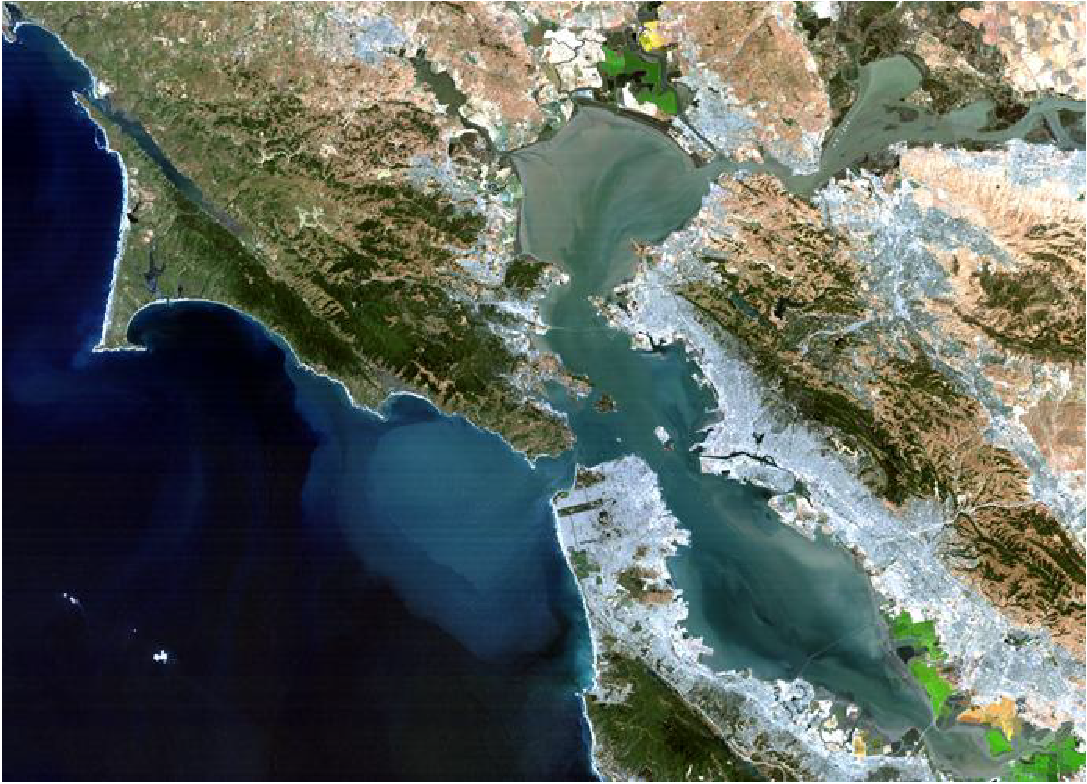
\includegraphics[scale=0.6]{image/plume2}
	\caption{Extent of sediment plume.}
	\label{fig:plume2}
\end{figure}

\begin{figure}
	\centering
		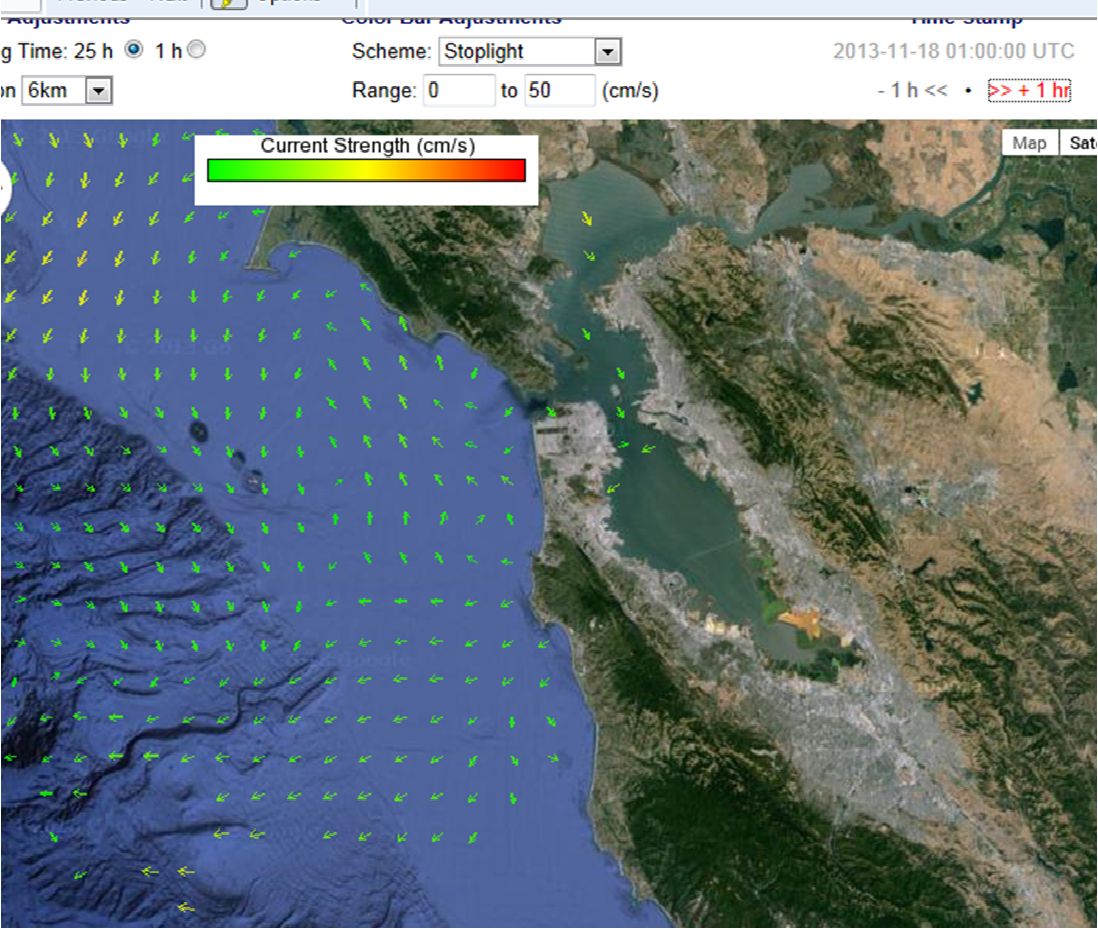
\includegraphics[scale=0.6]{image/hfradar.pdf}
	\caption{HF Radar surface currents (25 hour average, ****).}
	\label{fig:hfradar}
\end{figure}

\section{Flow Boundaries}
The main river inflows to the domain are shown in Figure ** and summarized in Table ***. As indicated, all our 
streamflows came from the USGS. Conductivity measurements were availble at some sites, others had to be approximated using
assumed constants or climatology as indicated in the table. The acquisition of the data involved some personal 
interaction and special requests and the subsequent processing is not easily reproducible, so it is our intention 
to release the data package for the calibration period along with the model. We also borrowed heavily from DSM2 inputs,
which have prepared in our section through 2011 and uses a lot of the data sources albeit with a greater reliance on
daily averaged data and CDEC as a data source. Occasionally there are large discrepencies between CDEC and USGS direct
sources of data; it just so happens that the beginning of our calibration in 2009 was one of those periods for Freeport,
with discrepencies reaching thousands of cubic feet per second (Figure ***).

As indciated in table ***, some data were made available to us as daily averages.
We interpolated the data using a rational histospline (****), which provides a (mostly) conservative, 
positivity and shape and peak preserving and accurate intepolation down to smaller time steps. 
Besides being inaccurate compared to this spline when applied to daily or monthly averaged data, 
the 24-hour square-wave produced by interpreting averages as flat lines can lead to results that are
subsequently misinterpreted as a daily or 14-day (through "`aliasing"') phenomenon. A 24-hour stairstep can also potentially influence model 
results at tidal frequencies and can degrade model performance due to the introduction of "`mini-tsunamis"' at the boundary. 


\subsection{Sacramento River boundary and extension}

\subsubsection{Boundary placement}
The upstream Sacramento boundary of the model is indicated in Figure ***.  The Sacramento River extends ***km north of I Street in Sacramento. Major tributaries have been lumped into the Sacramento channel, a point we will address again in our anticipated Yolo extension. The primary considerations for placement of the boundary were:

\begin{itemize}
	\item Availability of flow and bathymetric data
	\item Increasing complexity of the channel system (Yolo, Feather, American) north of I Street
	\item Need for the boundary to be free of tidal influence and boundary reflection
	\item Future extensions to Yolo requiring a boundary upstream of Fremont Weir.
	\item Performance and best practices with SELFE on upstream reaches
\end{itemize}

Of these criteria, the most constraining is the one concerning tidal influence and boundary reflection. Boundary reflection occurs when ocean tidal signals propagate all the way to the upstream boundary, conflict with incoming information and causes a reflected wave that moves back downstream and distorts conditions in the interior of the model. The effect of reflection on accuracy is significant and surprisingly far reaching. Figure *** shows the difference between model results at *** between a model truncated at I Street and a model extended beyond the zone of tidal influence near Knights Landing ****. Both models were forced by flows that were tidally filtered (ie, non-tidal in nature), which conflicts with conditions at I Street (see Figure ***) but not the upstream boundary. Clearly the effect of boundary reflection is felt as far as ***. For reference Figure *** compares water levels at I Street and the next available upstream gage at Fremont Weir demonstrating that the tidal signal is extinguished somewhere between these two sites.
 
\subsubsection{Boundary Data}

The simplification of flows into a single "`pseudo-Sacramento"' simplifies the system but requires a lumped estimate of flows into the Delta. In the Delta, the most upstream source of this combined flow is the USGS station at Freeport. We use data provided directly by the USGS because of large discrepencies between the USGS agency data and CDEC during the early months of our 2009 calibration period.  We also tidally filter the Freeport data, which has a significant tidal component that would be inappropriate if the data is lifted to the location of our boundary near Knights Landing. 

We use only flow and salinity to drive the model at the upstream Sacramento boundary. Overspecification using both flow and stage has been used successfully in Columbia River applications on steep river slopes, and is thought to help fix the upstream water levels at an appropriate elevation. Our only experiment with overspecification was at I Street where we found it was ****however we found that unless the flow and stage data are taken from 

\subsection{San Joaquin River}
The San Joaquin River Boundary is at Vernalis (Figure ***). As the contours in the figure show ***, south of Old River the San Joaquin transitions quickly from flat estuarine conditions to riverine. Field data indicates that Vernalis is naturally out of the zone of tidal influence. This is the the most important location in the Delta part of the model domain where flows are reported on the basis of stage observations and a rating curve. 

Unlike the field data, our model shows a small amount of tidal influence at the Vernalis boundary, indicating the model is a little underdamped in this part of the system. Some boundary reflection no doubt also results.

\subsection{Exports}
Export locations are indicated in Table ***. Our calibration period does not overlap with the CCC intake at **** . Data for the exports came from the original agencies or Dayflow, and the original data preparation comes from DSM2.

\subsubsection{Clifton Court and State Water Project}


\subsubsection{Contra Costa Water District}
The SELFE model was prepared to model three diversions at 


\subsection{CVP Tracy Pumping Plant}


\section{Delta agricultural sources and sinks}
The Delta islands are mostly agricultural, and diversions and returns of water from the islands significantly impact 
flow and water quality in the channels. The magnitude of the water quality impact varies with the seasons, as 
the balance between diversion, drainage and seepage changes. During summer months (including 2009), it is not
uncommon for the net sink of water due to consumptive use to exceed all of \gls{ndo}. This means that consumptive
use is not only a major driver of local water quality, but also a dominant contributor to the flow balance preventing
salinity intrusion from the ocean. 

Historical flow and water quality data has not traditionally been available for the islands. 
There have been recent efforts to map diversion pumps and return structures and it appears that many farmers in the Delta appear to log their diversions and returns now, but to the best of our knowledge these 
improvements have not yet been consolidated into a modeling product.  

\begin{figure}
	\centering
		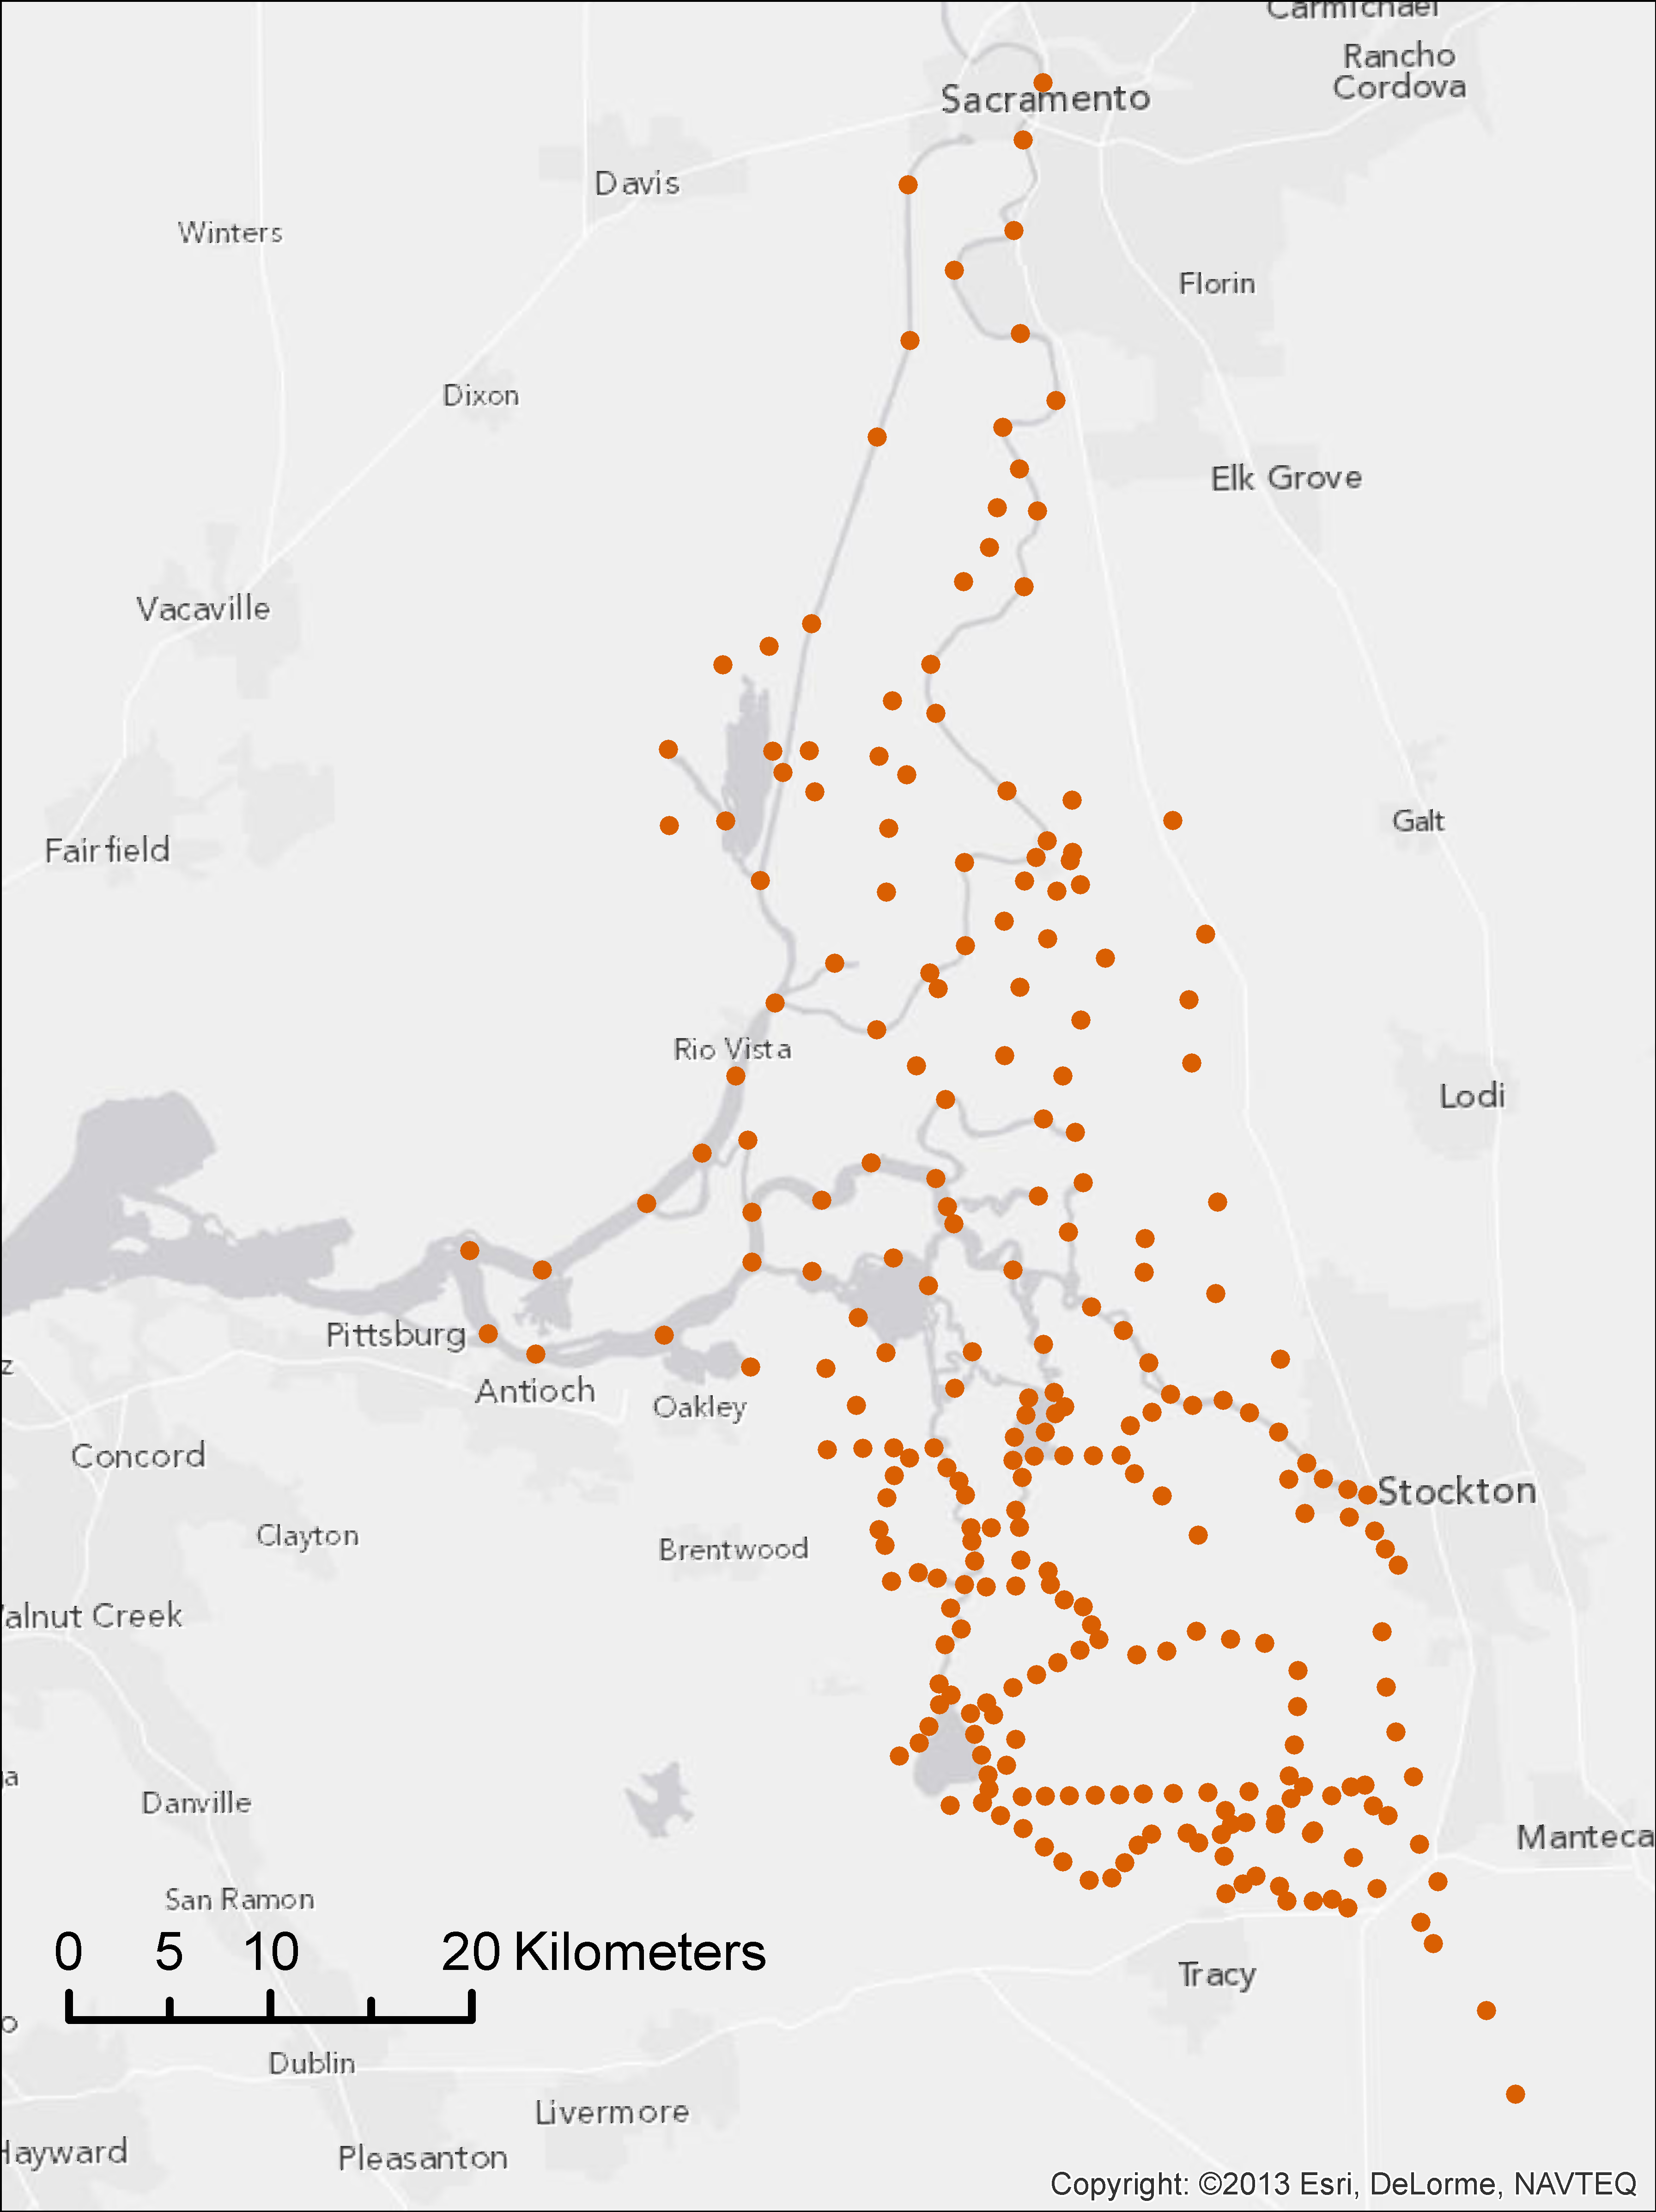
\includegraphics[scale=0.75]{image/dicu}
	\caption{Delta Island Consumptive Use diversion and return locations.}
	\label{fig:dicu}
\end{figure}

In the absence of field data, we use estimates from the DWR Delta Island Consumptive Use model
 (Mahadavan 1995, Jung 2000). The DICU model is centered on the islands (or regions), and performs 
a water balance that assumes land use and crop types and seeks to explain the resulting demand for water
in terms of precipitation, soil water balance, seepage and applied water.
The inferred fluxes to and from the Delta channels are then assigned to discrete locations in a second
step that is distinct from the water budget model. Although the assignment of locations 
is based on survey locations, the original locations are aggregated and the final locations of 
the sources are influenced by the location of nodes in \gls{dsm2}. The sites are shown in Figure \ref{fig:dicu}.

Delta consumptive use estimates can play an important part in model accuracy. 
During the summer months, agricultural water use can equal or exceed total
Net Delta Outflow in magnitude (Figure \ref{fig:ndo_vs_dicu}). Since outflow is a 
key quantity controlling salinity intrusion and consumptive use is the most uncertain
 components of outflow, DICU can play a controlling role in the accuracy of the model for salt.
In the one dimensional model DSM2, this error has been associated 
with overestimation of salinity in dry years including 2009. 

Because it is a monthly model, DICU also has difficulties representing event-scale runoff. 
DICU calculates runoff drainage based on excess precipitation (precipitation minus demand) 
and assumes that runoff is zero if there is no excess. The determination is made using monthly totals, 
which dilute short rainfall events over the full month and reduces the chances that they will be 
correctly identified as runoff. At best, the events are smeared in time; at worst, this 
miscategorization can trigger some accounting quirks with demand and cause volumes to be dropped altogether.

There is an event in mid-October of 2009 that illustrates how important isolated runoff events can be. This event
is shown in Figure \ref{fig:dayflow_oct_2009}, which plots Dayflow estimates of inflows, exports, precipitation and outflow for the latter part of 2009. The event in question begins on October 12, after which river inflows and exports go up modestly.
Because inflows and exports rise and fall roughly in tandem, their contributions to change in outflow tend to cancel out. 
Nevertheless, the Net Delta Outflow still goes up sharply because it is dominated by precipitation.
 
To examine the effect of runoff results, we simulated this period twice with identical parameters --  
once with DICU as-is and once substituting values from another consumptive use model \acrshort{detaw} during the storm period.
 \acrlong{detaw} is a daily water balance model for consumptive use that is still in development at DWR; it
is beyond the scope of this document to describe DETAW in detail, but we believe is more realistic for this type of event. 
Figure \ref{fig:detaw_vs_dicu} shows the difference between the two models in terms of agricultural drainage, which 
is the term that includes runoff. DICU ignores most of the volume of the storm and the rest is distributed over all of October.
DETAW, on the other hand, assumes that most of the precipitation that falls over the Delta contributes to drainage.

Figure *** shows the resulting model salinity results at several stations in the Bay and Delta. The simulation
based on DICU inputs do well until the storm, but after the event salinity remains high on as if nothing had happened. In 
contrast, salinity is driven down system-wide both in the DETAW driven model and in the field data. A difference of
3-4 psu (perhaps 4000***) develops immediately after the event in the west Delta and Bay stations and lasts for 2-3 months. 
Since the west corridor is the gateway to the Delta, the anomaly eventually reaches every Delta station. In contrast to 
any summer seasonal inaccuries in Net Delta Outflow, we found this issue to be very easy to identify with confidence, and we
retained the higher drainage for October and December for our calibration.

Up to now, we have described uncertainty due to consumptive use through the mechanism of salinity intrusion.
In addition, there is considerable uncertainty concerning the salinity of agricultural returns in early storms. 
Large spikes in of salt and other constituents occur following {\em first flush} precipitation 
events after dry periods. These spikes are evident in the historical records at mid and South Delta monitoring stations, and the sources and quantities involved have not been well characterized.

\begin{figure}
	\centering
		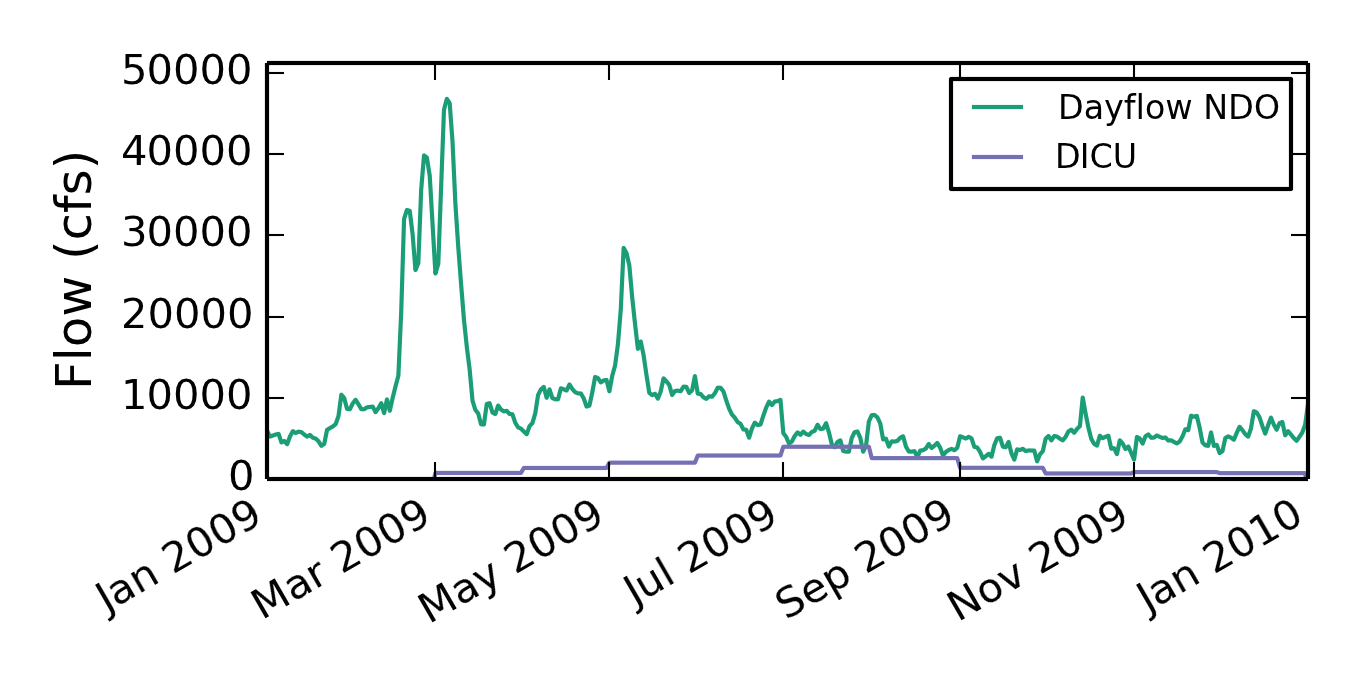
\includegraphics{image/ndo_vs_dicu}
	\caption{Net Delta Outflow and Delta Island Consumptive Use estimates for 2009.}
	\label{fig:ndo_vs_dicu}
\end{figure}

\begin{figure}
	\centering
		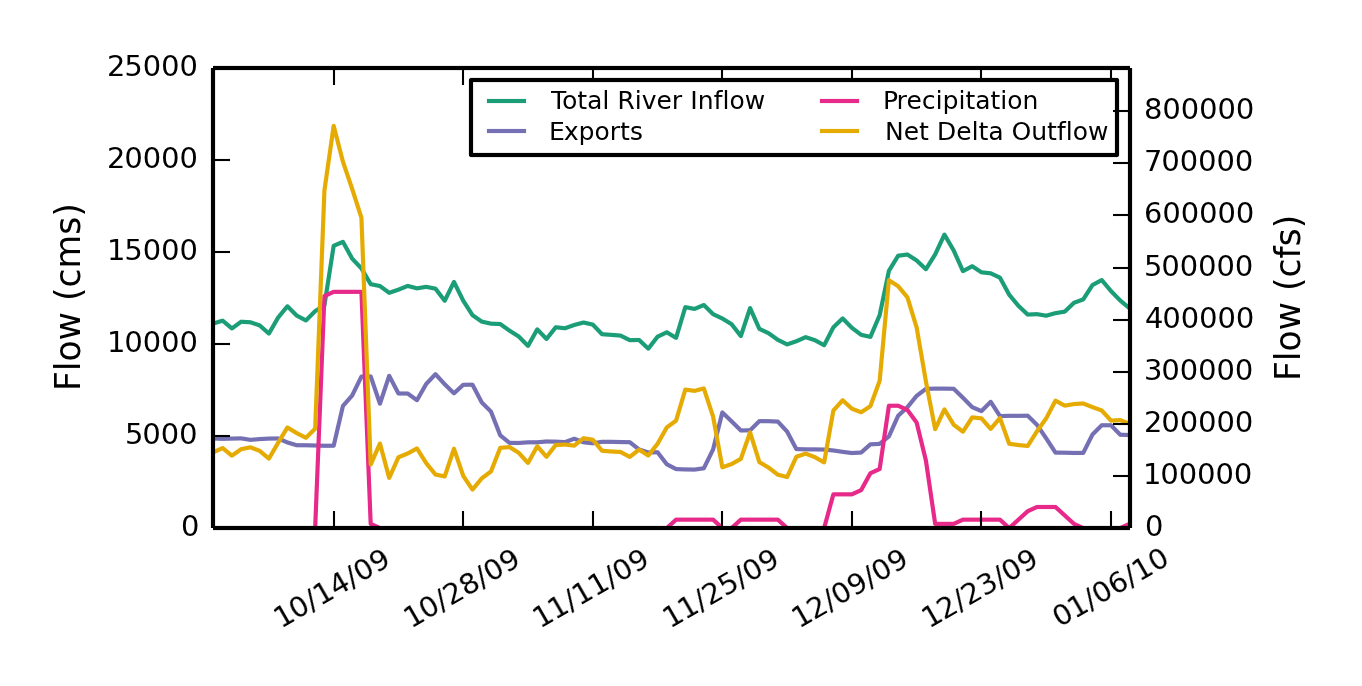
\includegraphics{image/dayflow_oct_2009}
	\caption{Dayflow estimates of inflows, exports, precipitation and Net Delta Outflow for the last part of 2009,
	including the storm period in mid-October.}
	\label{fig:dayflow_oct_2009}
\end{figure}

\begin{figure}
	\centering
		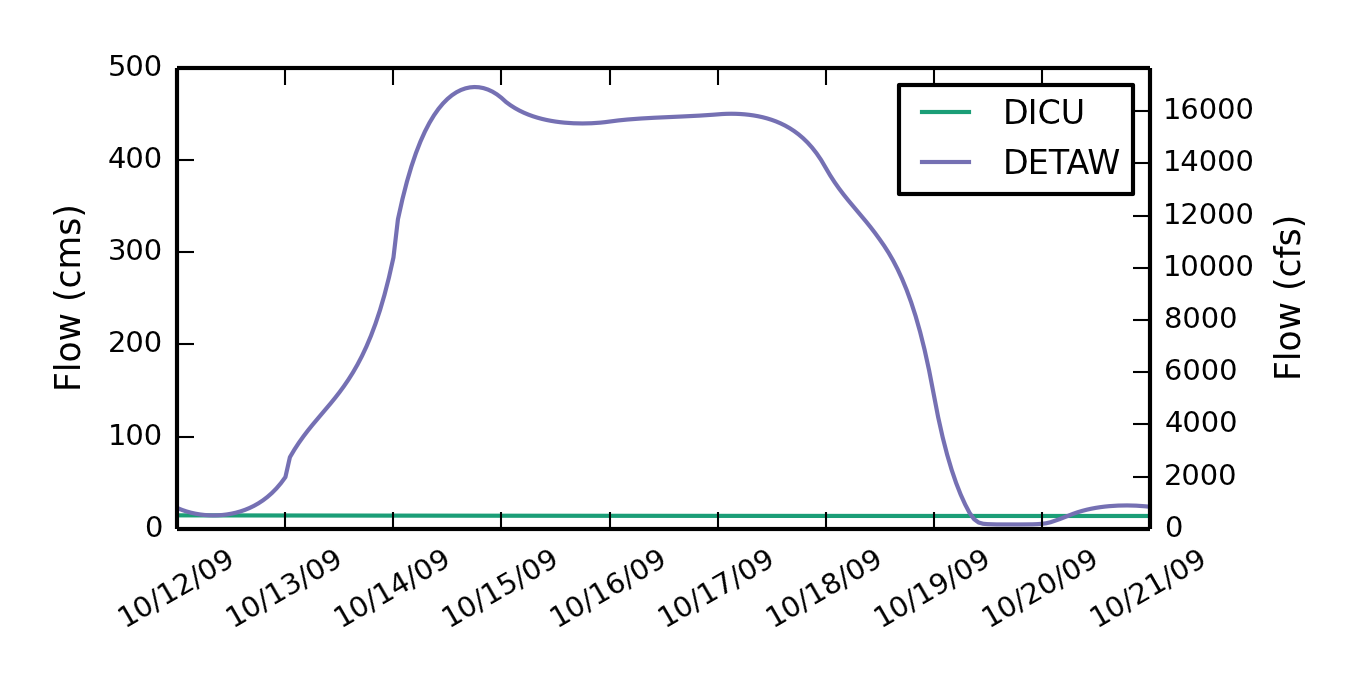
\includegraphics{image/detaw_vs_dicu}
	\caption{Estimates of agricultural drainage from DICU and DETAW around the period of the storm.}
	\label{fig:detaw_vs_dicu}
\end{figure}


\section{Atmospheric inputs}
When modeling flow and salinity transport, SELFE accepts spatiotemporal atmospheric 
input representing surface wind, atmospheric pressure
and precipitation over the domain. The most significant of these is thought 
to be wind, which alters flow patterns and induces mixing
resulting in as much as a 2 psu difference in salinity at Martinez. There is no unified approach to
modeling wind in the Bay-Delta region. Past work in the domain has either justified neglecting 
wind due to a short period of study \citep{Chua2011}
or used atmospheric inputs from a small set of representative 
stations situated on the water \citep{MacWilliams08,MacWilliams09}.

The approach we adopted is to use climate or weather reanalysis products that 
combine both a physical model and data assimilation. 
Numerous reanalysis products are available for the region at both climate 
(coarser) and weather (finer) scales. For our calibration we used winds
at 10m above ground from the \gls{narr} 
dataset from NOAA. This dataset is 32km in resolution, which is roughly 
the spacing of field stations used in \citep{MacWilliams08,MacWilliams09} and not fine enough
to resolve the width of the Bay or local spatial patterns of wind at 
the Golden Gate, South Bay, San Pablo Bay and Carquinez.

Through our collaborators in the SESAME project, we have access
to two much finer resolution wind fields 
from reanalysis products. The first is a 3km COAMPS model from the \gls{cencoos}. 
The second is a 1km WRF simulation from NASA unique 
to the SESAME project. The results of our collaborators indicate that the 3km model is able 
to reproduce many of the spatial features of the winds on the Bay, but
tends to reduce magnitudes, a common issue and certainly one that the NARR dataset suffers
from as well. The 1km model has higher peaks, but it was unclear to our collaborators 
that sensitivity for modeling justified the expense (months of supercomputer use) spent generating the 1km
product. 

The importance of atmospheric forcing must be balanced against the uncertainty and noise surrounding wind, 
the unknown (and relatively unknowable) effects of gusts and the expense of improving the wind and pressure data. 
Our principle goal in this project is to establish a robust model that can be used to examine hypothetical 
planning questions or future conditions. The calibration results presented 
in this document for the Bay suggest this is possible for scenarios that 
do not involve changed atmospheric conditions; to quantify our confidence for climate change scenarios 
involving big changes in the frequency of barometric events, further sensitivity analyses are required.


\section{Delta hydraulic control structures}
\label{sec-delta-structs}
Radial gates, barriers, culverts and other hydraulic structures are used in the the 
Delta and Suisun Marsh to help manage water quality, protect fish migration, maintain 
agricultural water supply (head) in the South Delta and control storage at Clifton Court. As part of this project
we added the ability to model a variety of such structures to SELFE. The implementation, 
which borrows concepts from DSM2 and HEC-RAS, uses fundamentally
1D parameterizations to allow the embedding of the structures in 
an otherwise medium resolution multi-dimensional mesh. More details are described in 
Section \ref{sec-structures}. 

Many structures in the Delta are seasonally installed or operated. Figures \ref{fig:gate_schedule_2009}
and \ref{fig:gate_schedule_2010} shows the operational schedule for 2009. 
Additional detail on what these operations mean is given 
in the individual control structure descriptions.


\begin{figure}
	\centering
		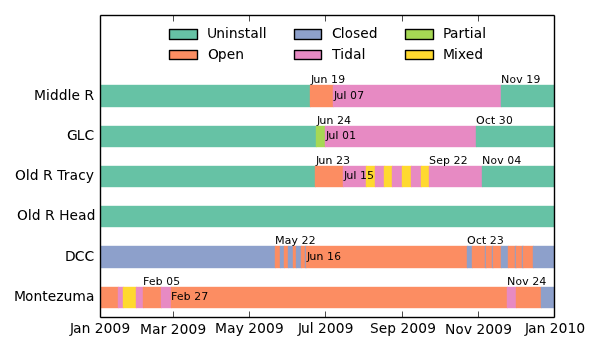
\includegraphics[width=\textwidth]{image/gate_schedule_2009}
	\caption{Delta hydraulic structure operations for 2009.}
	\label{fig:gate_schedule_2009}
\end{figure}

\begin{figure}
	\centering
		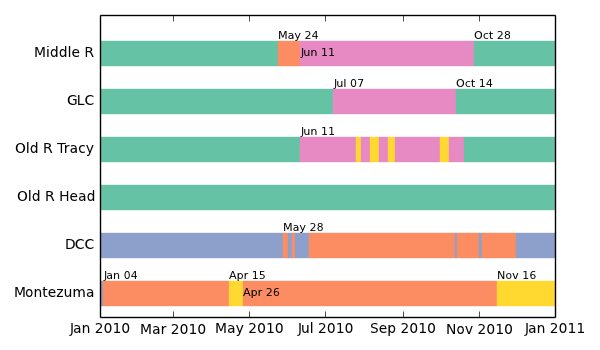
\includegraphics{image/gate_schedule_2010}
	\caption{Delta hydraulic structure operations for 2010.}
	\label{fig:gate_schedule_2010}
\end{figure}


\subsection{Delta Cross Channel} The \gls{dcc} is a permanent structure on the 
Sacramento River that comprises two 36.6m (120 ft) wide radial gates. The gate, along with the 
6,000ft cross channel connecting the  was completed by the \gls{usbr} in 1950-1951. The gate is 
opened in order to freshen water in the central Delta as well as for recreational boating use. 
The \gls{dcc} is operated seasonally with mandated closures to protect fisheries 
under \gls{d1641} and operational closures during periods of high flow to prevent scour. 

The openings and closings for our period of interest are given in 
Figures \ref{fig:gate_schedule_2009}-\ref{fig:gate_schedule_2009} and
 and are taken from the USBR historical log. In recent years, including the calibration period, the gate has 
remained closed for fish protection until Memorial Day weekend. In 2009, the cross-channel was 
open from June-October, although it was toggled open and closed frequently at the beginning and end of
that season. 

During the calibration period, the \gls{dcc} was operated with both gates either fully open or closed. 
This is the most common mode of use, although in the months before our calibration experiments 
were conducted with the gates operated frequently and sometimes in a partially open state. 

We model the cross channel as a radial gate. Flows through the channel 
seem to match observations well. We are not aware of any official gate rating for the cross-channel, 
although in a presentation before the \gls{cwemf} in 2006, K.T. Shum of EBMUD 
described problems in the fit of radial gate equations and advocated the use of 
flow contraction equations instead, such as those given by \citet{Matthias67}.
We have so far not been able to reproduce the difficulties leading to these comments.

\subsection{Clifton Court Forebay Gates} Five radial gates control flow into the Clifton Court Forebay. The gates are each *** wide (**m), with a sill elevation of *** m NAVD (**** ft NAVD ,or *** ft NGVD). Each of the five gates can be independently operated although they are most commonly operated in tandem. 

The gates are operated in accordance with an agreement with the South Delta Water Agency to maintain water levels in the surrounding region. The resulting {\em Priority System} describes when in the tide cycle the gates may be opened. The priorities schedule is shown in Figure ***. The most common priority is {\em Priority 3}, which under normal tidal circumstances allows the gates to open 1 hour after the lower low tide, close 2 hours after the higher low tide, open again 1 hour before the higher high tide, and close 2 hours before the next lower low tide. This schedule specifies the maximum periods when gates may be opened to inflow; the gates can be closed early if daily inflow quotas have been met and the gates are always closed to outflow.

\begin{figure}
	\centering
		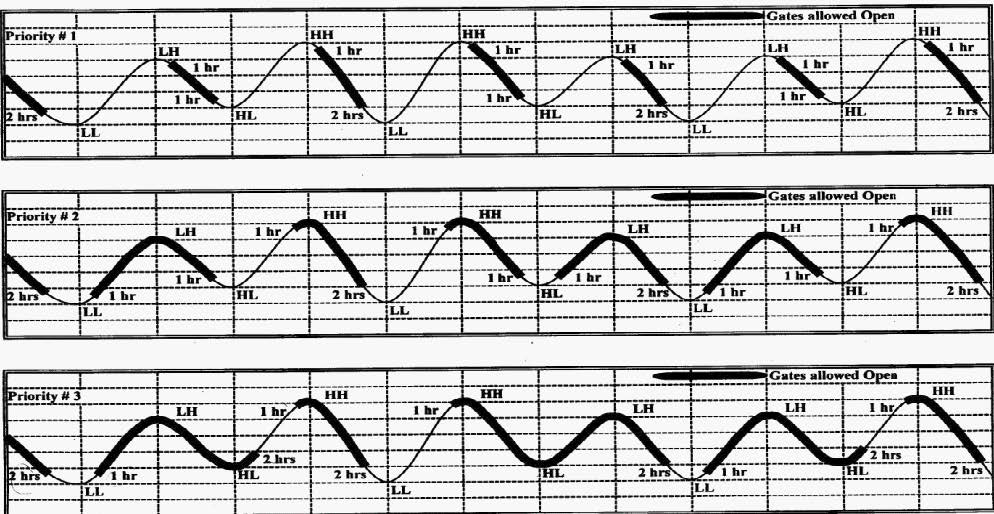
\includegraphics{image/ccfb_priority}
	\caption{Clifton Court Gate Priority Schedule.}
	\label{fig:ccfb_priority}
\end{figure}

Unlike other radial gates in the system, the CCFB gates are often operated such that the upstream side of the gate is submerged and the downstream side is submerged or (possibly) partially submerged. The term {\em partially submerged} is based on the state on the interior side and refers to the transition between {\em free flow} and {\em submerged flow} cases as indicated in Figure \ref{fig:radial_gate}. Partial submergence is something of a grey area in the literature on radial gates -- it is a regime that is difficult to characterize or even identify. Traditional measures of partial submergence, such as those implemented by the Army Corps of Engineers HECRAS, are based on the ratio of tailwater to headwater ($0.6 < y_3/y_1 < 0.8$). This ratio almost always exceeds 0.8 at Clifton Court, so by this criterion the gate is always fully submerged. More recent work on radial gates \citep{Clemmens03,Wahl05} interprets submergence based on whether downstream flow depth is greater than the theoretical free-jet thickness for a given gate opening. This leads to a more greater likelihood of characterization of partial submergence.

Operations near the partial submergence threshold make it challenging to develop a flow rating that applies well over the full range of gate heights and water levels. The DWR \gls{dfd} has a set of equations developed by \cite{Hills1988} that have been cited extensively, but these equations were developed over a very limited range of gate heights and are thought to be in error by as much as 40\% under some conditions. The DWR Delta Field Division calculates these values at ten minute intervals, but we are not aware of any circumstances at the DWR where the resulting flows are used without significant reinterpretation. The Delta Modeling Section is been developing a new rating for the gate for some time, but the collection of data for certain flow and stage combinations has been delayed by operational changes and a mechanical failure at one of the gates. DSM2 uses an orifice equation calibrated heuristically based on storage changes in Clifton Court; we believe this is a justifiable single-equation approach, but have not yet had an opportunity to verify how well it reproduces fluxes into Clifton Court.

For historical calibration (as opposed to hypothetical scenarios), the issue of improving the gate rating can be deferred because other supporting data are available. \citet{MacWilliams13} suggest a methodology whereby the ten minute Hills equation gate flows are scaled on a daily basis to match the historical daily flux into Clifton Court estimated by Dayflow. The Dayflow estimate is based on a mass balance on the reservoir that includes daily fluctuations in CCFB water levels, \gls{swp} and \gls{bbid}. We did not include an evaporation correction. The resulting flows reproduce the daily volume in CCFB by definition, and can be prescribed directly in SELFE using a {\em flow transfer} (see Section \ref{sec-transfer}). The main difficulty we encountered with this approach was that the flow balance between the gates and pumps is delicate and easily disrupted by things like interpolation techniques or FEM mass conservation errors -- a long term average bias of 1 cms will accumulate to a very appreciable drift in CCFB water levels.

\begin{figure}
	\centering
		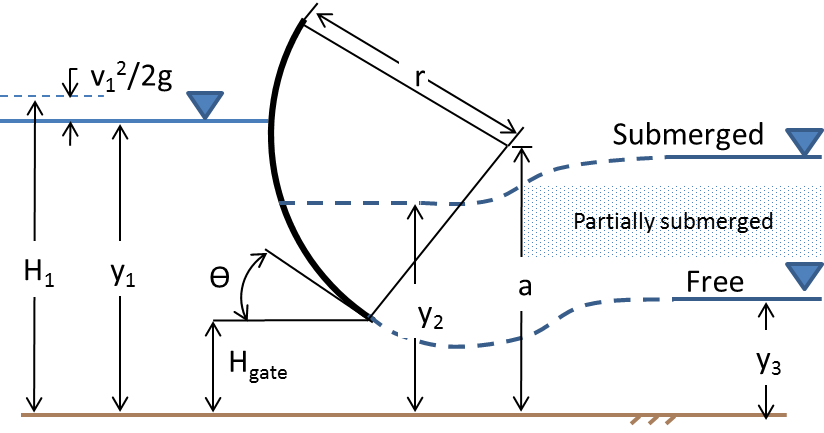
\includegraphics{image/radial_gate}
	\caption{Free and submerged downstream flow through a radial gate. The upstream is submerged}
	\label{fig:radial_gate}
\end{figure}


\subsection{Montezuma Slough Salinity Control Gates}
The Suisun Marsh Salinity Control Gates facility consists of three 11m (36ft) wide radial gates, a 36.6m (120ft) set of
flashboards and a 6.1m (20ft) wide boat lock. 

The gate is designed to operate tidally, restricting flow of higher salinity water 
from Grizzly Bay into Montezuma Slough on the incoming tides, and passing lower salinity 
Sacramento River water during ebb tides. Tidal operation of the gate lowers salinity 
in Suisun Marsh channels and results in a net movement of water from east to west. When the gates
 are left open and \gls{ndo} is low, the net movement is slightly west-to-east.

The salinity control structure radial gates can be operated operated tidally beginning in in early 
October and, depending on salinity conditions, may continue operating in this way 
through the end of the control season in May. As shown in Figure \ref{fig:gate_schedule_2009} and \ref{fig:gate_schedule_2010} 
the window of tidal operation in 2009-2010 was actually just a few months. 

The flashboards are wide stoplogs that can be removed to allow unimpeded flow when salinity conditions in the Marsh are favorable. The boat lock tends to be held open when the flashboards are in to allow improved fish passage and is closed when the flashboards are out. 

The Bay-Delta SELFE model includes all three subdevices at the control structure. 
The weir is modeled using a radial gate using the HEC formulation. Coefficients were taken from
the DSM2 inputs and were not adjusted. The boat lock is modeled as a weir, and the flashboards as a rectangular orifice. 
Dimensions and coefficients for these structures were also borrowed from 
DSM2 inputs. 

\begin{figure}
	\centering
		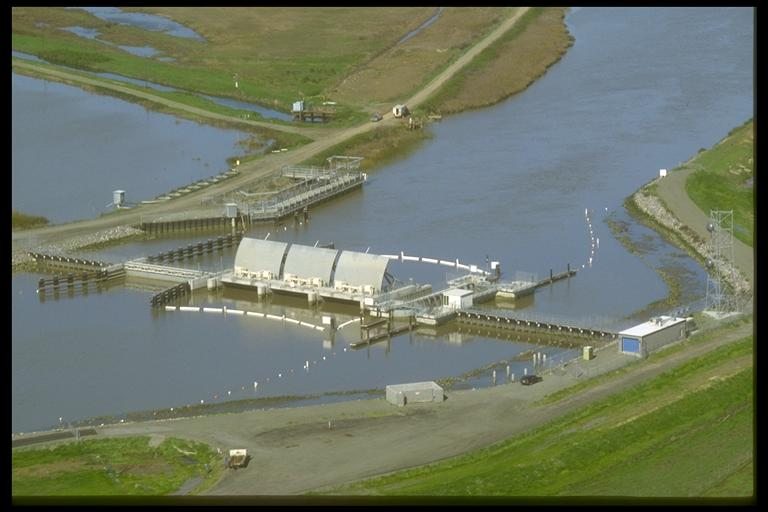
\includegraphics[scale=0.5]{image/smscg}
	\caption{Montezuma Salinity Control Gate.}
	\label{fig:montezuma}
\end{figure}

\subsection{South Delta Temporary Barriers} The South Delta Temporary Barriers have been installed in
various configurations in four locations in the South Delta since 1991. They include one fish barrier 
at the Head of Old River and three seasonal rock barrier sites on Middle River, Grantline Canal and Old River (Figure **). The fish barrier is intended to protect migrating San Joaquin River Chinook salmon from being entrained by 
water project pumps. The three agricultural barriers are intended to preserve water levels 
and improve water quality in the South Delta for agricultural water users along those channels. 

The agricultural barriers are all designed in roughly similar way, including a rock barrier 
with a crest above sea level as well as a set of 4ft diameter (1.22m) diameter 
culverts with optional flap gates for tidal operation.  The configuration of the culverts varies by
site: the Middle River has three at the north levee side and three at the south side, the GLC barrier 
has all six culverts on the south levee side, and the Old River barrier has all nine culverts situated in the middle
under the weir. At Middle River and the Grantline Canal barriers, the bank of culverts stay in year round.
In all cases, weir and pipe flow are summed as if they were independent, ignoring the complications 
arising from interaction. Porosity of the rock barriers themselves is also ignored.

To the best of our knowledge, the flow coefficients of the agricultural barriers 
have not been studied in isolation -- ie, by observing velocity directly upstream 
or downstream using \glspl{uvm} or \glspl{adcp}.
We began by using weir and culvert coefficients from DSM2, but found that these coefficients
were high in the context of SELFE (and indeed are high according to published recommendations). This
 seems particularly true in before the culverts were replaced in 2010-2011. As a result, we reduced both culvert and
weir coefficients to less than half their original values.

\section{Domain variations (Bay-only, Delta-only)}
Although the final 'production' simulations were carried out on the Bay-Delta grid, 
we also conducted some earlier experimental work with Bay-only grids, in order to sort some 
calibration issues in the lower estuary more efficiently. The grid (Figure ***) 
is much smaller than the Bay-Delta grid, with only ~23K nodes. This allows much 
quick turn-around time for experiments involving Bay dynamics. The model skills are 
largely comparable on the two grids, with slightly better results from the larger grid, 
partly due to the reduction of reflection at the river boundaries
and natural exchange through Threemile Slough. For the Bay-only
grid, the river boundaries are located at Jersey Point and Rio Vista, with measured stages, flows and EC imposed there. 
No "False Delta" was used as was the case in early work by most other authors.

Also of interest to the Department is a Delta-only domain with a boundary at Martinez -- possibly
with less vertical resolution or even in 2D. SELFE has often been used in this way and
we have developed scripts to perform the necessary kind of domain chopping, 
but our focus thus far has been on the full domain in 3D.

\section{Domain-specific sources of uncertainty}
The current state of the model encompasses many important facets of the Bay-Delta system, particularly the upper estuary and Delta where operational details can be most critical. Nevertheless, some details of the Delta remain unknown difficult to model
  \subsection{Delta consumptive use}

	
	\subsection{Bathymetry}
  The present project has advanced the 

	\subsection{Vegetation and friction}
	



\chapter{Calibration}
\label{chap:calibrate}
\section{Calibration variables}
The purpose of a hydrodynamic calibration is to ready the model for the domain or application, 
as well as gain insight into its suitability for general modeling purposes.  This insight can then 
be quantified by validating over a longer period in which the model is not adjusted. Calibration 
and validation are always indicated for a new model application; they may also be indicated when 
new physical processes (sediment, biogeochemistry) are added, additional focus
is required of a subarea of the domain or new data becomes available.

This calibration covers hydrodynamic variables (water surface, velocities and cross-sectional flows) as well as salinity.
The calibration does not include temperature, although our collaborators on the SESAME project have done extensive work in the Bay on temperature and we expect to publish results on temperature over the full Delta soon.

Salinity (and conductivity) are among the best monitored constituents in the system. 
Salinity is a conservative tracer, meaning that it is not consumed or created by reactions with other 
constituents, affected by heat flux or interactions with sediment. All conservative tracers 
are transported by the same physical processes, so that in principle a salt calibration should 
apply to other conservative constituents such as bromide or \gls{doc} as well as providing the foundation
for modeling nonconservative constituents such as dissolved oxygen and mercury. Inasmuch as there are
differences between salinity and other constituents this is because of the role of the ocean boundary.
Most salinity in the Delta is carried up the estuary through tidal and estuarine mixing processes such as gravitational circulation. 
With DSM2, the Delta Modeling Section has found it insightful to model \gls{doc} as well, precisely because
is not dominated by ocean sources. This allows a greater focus on other components of transport; it also makes
\gls{doc} more robust to errors in consumptive use estimates.

\section{Calibration parameters}
Although calibration is often liked to turning knobs, the process of calibrating a 3D unstructured 
grid model with ten million or more state variables involves numerous activities that don't amount to parameter adjustment. 
For instance, much of the project development time involves adjusting, refining and balancing the mesh or collecting
and incorporating improved bathymetry. Even when we do adjust the model, selecting or swapping algorithmic options is often more influential than, say, adjusting friction. 

Although we did some experiments with other parameters, the main items that we manipulated in the calibration were these:
\begin{itemize}
	\item horizontal mesh configuration and density
	\item vertical mesh selection, configuration and density
	\item roughness coefficients
	\item the selection of turbulence closure
	\item the choice between higher order and linear ELM
\end{itemize}

We experimented with several relationships between roughness or drag and depth, but we applied the same formulas
over the entire domain -- we did not consider spatially varying friction formulas. 
Using different roughness or even different turbulence closure might be appropriate for based
on the presence of bedforms or vegetation, but these distinctions would involve additional data collection and 
introduce seasonality. We may visit these ideas in the future for detailed study regions where more complete observations are available concerning horizontal and vertical velocity structure and lateral distribution of tidal phase.


\section{Calibration period and time step}
The period of the the calibration period covered in this document is March 12, 2009 to ****, 2010. The year 2009 is categorized as Dry and 2010 is categorized as Below Normal. We used the period March 12, 2009 as the start date because of the availabilty of USGS cruise data for salinity initial conditions.
The period through Fall 2009 was used as the basis of adjusting parameters. The bulk of 2010 was used for validation.

The hydrodynamics time step is 120 seconds for all the simulations. This time was decided early in the project on the basis of sensitivity runs on the Bay-only variant of the mesh and is in keeping with the 
\gls{cfl} minimum time step to avoid numerical diffusion in the the Eulerian-Lagrangian 
component of the algorithm (see section ***). The scalar transport 
part of the code is based on a different CFL time step restriction, this one a maximum rather than a minimum, 
and as a result the transport regularly subcycles the main hydrodynamic time step using steps between 3 and 20 seconds.

\section{Skill metrics for scalar station data}
For station observations of scalar quantities such as stage and flow, 
we evaluated model performance based on both visual assessments of time series plots and 
quantitative fitness scores. 

Each station analysis includes 14-day dynamic plots revealing tidal characteristics 
at the site over spring and neap conditions, as well as longer plots of tidally filtered results showing the
system response to longer period fluctuations such as barometric events and seasonal
inflow changes. For the tidally filtered plots, infrequent small gaps 
in the observed records were filled using interpolation in order to avoid the widening 
of the gaps to days that occurs when missing data are filtered. 

Below the time series plots are scatter plots of the phase-adjusted model results 
and observed data fitted with a regression line. The slope of the regression line has been
described by \cite{MacWilliams08} as a measure of signal amplitude amplification for tidal oscillations
and by \cite{Murphy88} as a measure of conditional bias (e.g., flow bias that grows or shrinks with flow).  
We also record the correlation coefficient (the square root of ${R^2}$) for consistency with other models
that also record this statistic. We do this with some hesitation given the shortcomings of the statistic in the current context
-- for serially correlated data this statistic occupies a narrow scale \cite{Ralston2006}, neglects important aspects of fit
\citep{Murphy88}. It also may give false positives or medium-high scores for nearly random predictions \citep{Ralston2006}
and does not appear to be informative in the presence of patterned errors such as would occur in a tidal environment. 

The scale of the scatter plots gives a good indicator of the total variability in the data 
including both tidal and non-tidal components. It can be contrasted with the scale of the 
tidally-filtered time series plots, whose y-axis is a good indicator of the variability of
the subtidal part of the signal. The scale of the dynamic plots was a compromise -- we used the 
natural range of the dynamic period data but constrained the range to be at least as large 
as that of the filtered data. 

We also evaluated fitness scores for important aspects (bias, fit, skill, phase) of 
model performance. The following statistics are reported where
appropriate:

\begin{description}
  \item{{\textbf{RMSE}}} Root mean square error. Note that unlike the other statistics 
	below marked with a $\phi$ subscript (and published calibrations from other models), 
	the data are not phase-corrected for this statistic.
  \item{{\textbf{Lag}}} An estimation of lag based on cross-correlation analysis, 
	similar to that described in RMA (2005) \cite{RMA05}. The idea of this analysis is to shift
	the model results forward and backward in time until the maximum cross-correlation 
	between the two series is obtained. A positive lag indicates that the model trails the
	field observations in the timing of tidal signals. The effectiveness
	of this statistic depends on the strength of the tidal signal compared to noise and longer term trends with vague     
	periodicity. The analysis was not performed for Delta salinity stations.
	\item{\textbf{Bias}\subphi} The median bias  of phase corrected error (modeled - observed)
	\item{\textbf{NSE}\subphi} The Nash-Sutcliffe efficiency for the phase-corrected error:
	\begin{gather}
	NSE\subphi(f,r,x) = 1 - (MSE(f,x)/MSE(r,x)) \\
	\text{where} ~ MSE(f,x) = \frac{1}{n} \sum\limits_{i=1}^{n}(f_i - x_i)^2 \\
	\end{gather} is the mean squared error between a forecast ($f$), an observation ($x$) 
	and a {\em reference forecast}. The choice of 
	reference forecast can several possible skill scores -- 
	the Nash-Sutcliffe is the simplest with $r$ representing the station time-average.
	\item{\textbf{r}\subphi} The correlation coefficient (the $r$ in $R^2$ for the fit 
	of the observations on the phase-corrected model values.
\end{description}


In addition to covering the major facets of accuracy in a tidal
system, the main criteria for these metrics were robustness and consistency with
other Bay-Delta model calibrations. The variety of published skill metrics for hydraulic and hydrologic models is extensive 
(some examples are \citet{Willmott82,Willmott85,Willmott12}, \cite{Stow09}, \cite{Murphy88}, \cite{Ralston2006}). 
No standard has emerged \citep{Stow09}, and there seems to be some schism between practitioners who work with 
measures of accuracy (e.g. RMSE) and those who work with skill. 

For systems with periodic forcing such as an estuary, many of the above statistics are sensitive to the phase 
(time shift) of the model relative to the observations. If this error is not controlled, 
it reduces the diagnostic value of the suite because the statistics would not differentiate an excellent
tidal signal with a modest shift from a shabby tidal signal. 
Following  RMA (2005) \cite{RMA05}, we first estimate phase error and then correct for phase (by shifting the model output in time) 
when generating the remaining statistics except for RMSE which is left as a composite indicator of overall error.

The metrics are not decomposed into tidal and subtidal time scales. This means that the diagnostic 
that the underlying physics and time series plots do. Subtidal and tidal information can therefore
obscure one another. In particular, tidal signals are generally much larger than the variation
of longer period fluctuations. When the two are mi

\section{Station inventory and descriptions}
The locations of stage, flow and salinity stations is shown in Figures ***. 
We relied on data from the following agencies and programs (method of retrieval is shown in parentheses):

\begin{itemize}
  \itemsep1pt \parskip0pt \parsep0pt
	\item NOAA (automated retrieval)
	    \subitem Verified Water Levels from ***
			\subitem Conductivity at *** stations in the Bay.
	\item USGS (request)
	    \subitem Conductivity from the Water Quality and Sediment *** Group
			\subitem Flow, stage and (post-2010) water quality from the Delta Hydrodynamics Group in West Sacramento
			\subitem CTD (conductivity-temperature-depth) cast data from cruises conducted by ***
  \item CenCOOS surface HF Radar
	\item DWR North Central Regional Office or NCRO (Water Data Library) 
	    \subitem Flow
			\subitem Surface Water Monitoring Program
			\subitem Water Quality Monitoring Program
	\item DWR Compliance* and IEP (request) for conductivity monitoring at **** sites
	\item DWR O\&M (CDEC) for operational data and pumping rates
	\item USBR (CDEC) conductivity and temperature stations in the Delta
\end{itemize}

In each case we report the station name, agency identification and CDEC identification for familiarity. 
\vfill
\section{Stage Results}
	   
  \subsection{Monitoring stations}
  \subsection{Tidal phase and amplitude}
	  Figures \ref{fig:m2_amp} - \ref{fig:k1_phase} map the evolution of the two 
		largest tidal constituents, M2 and K1, through the Bay-Delta 
		system for both model and observations during the month of ***. The amplitudes are labeled in meters, 
		phase is in terms of minutes difference from the timing at the Golden Gate. 
		
		The development of the tide through the Bay is generally accurate for M2; 
		there is an 11 minute delay in K1 at the San Francisco 
		station ***** but accuracy is good at most stations.
		
		Upstream in the Delta, there is a tendency for the tide to be underdamped -- the model overestimates 
		tidal amplitude and is early for phase at most stations. The error is regionally consistent, 
		meaning that stations nearby one another in the Sacramento, San Joaquin, 
		and Old and Middle River regions have similar characteristics. 
		Dampening can be increased roughness or by use of linear interpolation at the feet of characteristics
		in ELM, which is diffusive, but either measure entails reduction in the tidal range of flow. 
				

\begin{figure}
	\centering
		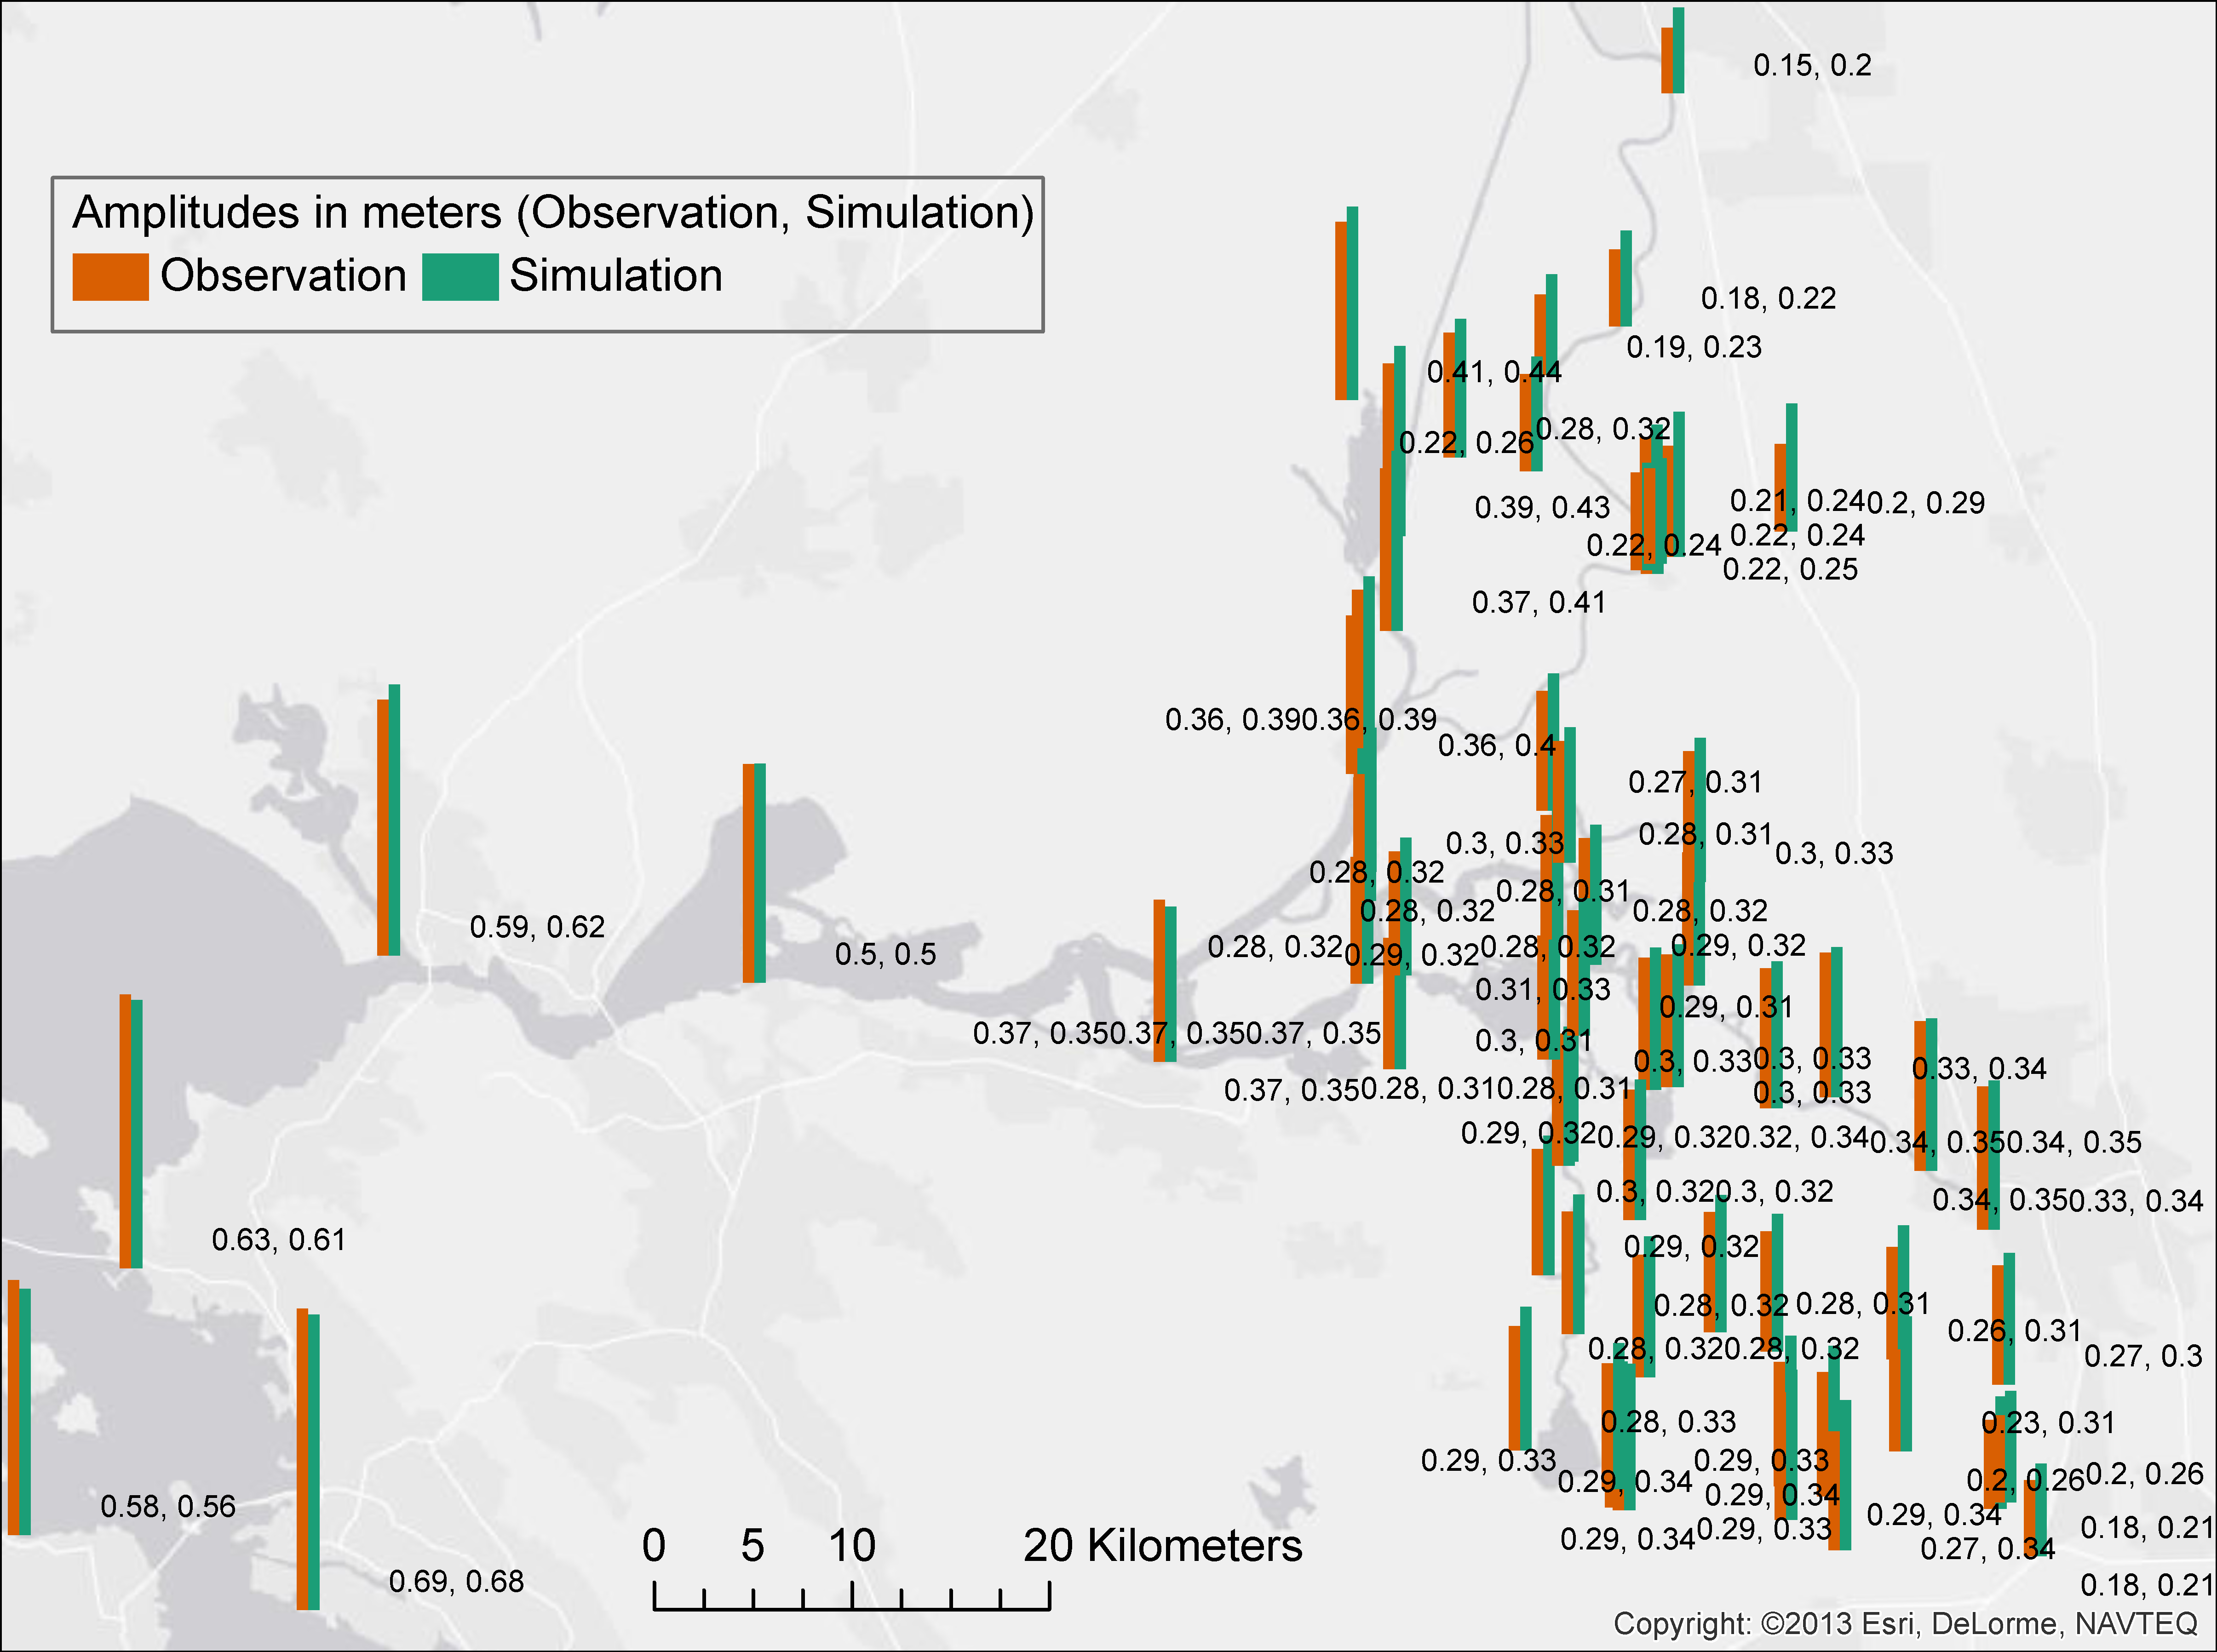
\includegraphics[width=\textwidth]{image/M2_amp_spatial}
	\caption{Map of M2 amplitude at Bay-Delta stations.}
	\label{fig:m2_amp}
\end{figure}
\begin{figure}
	\centering
		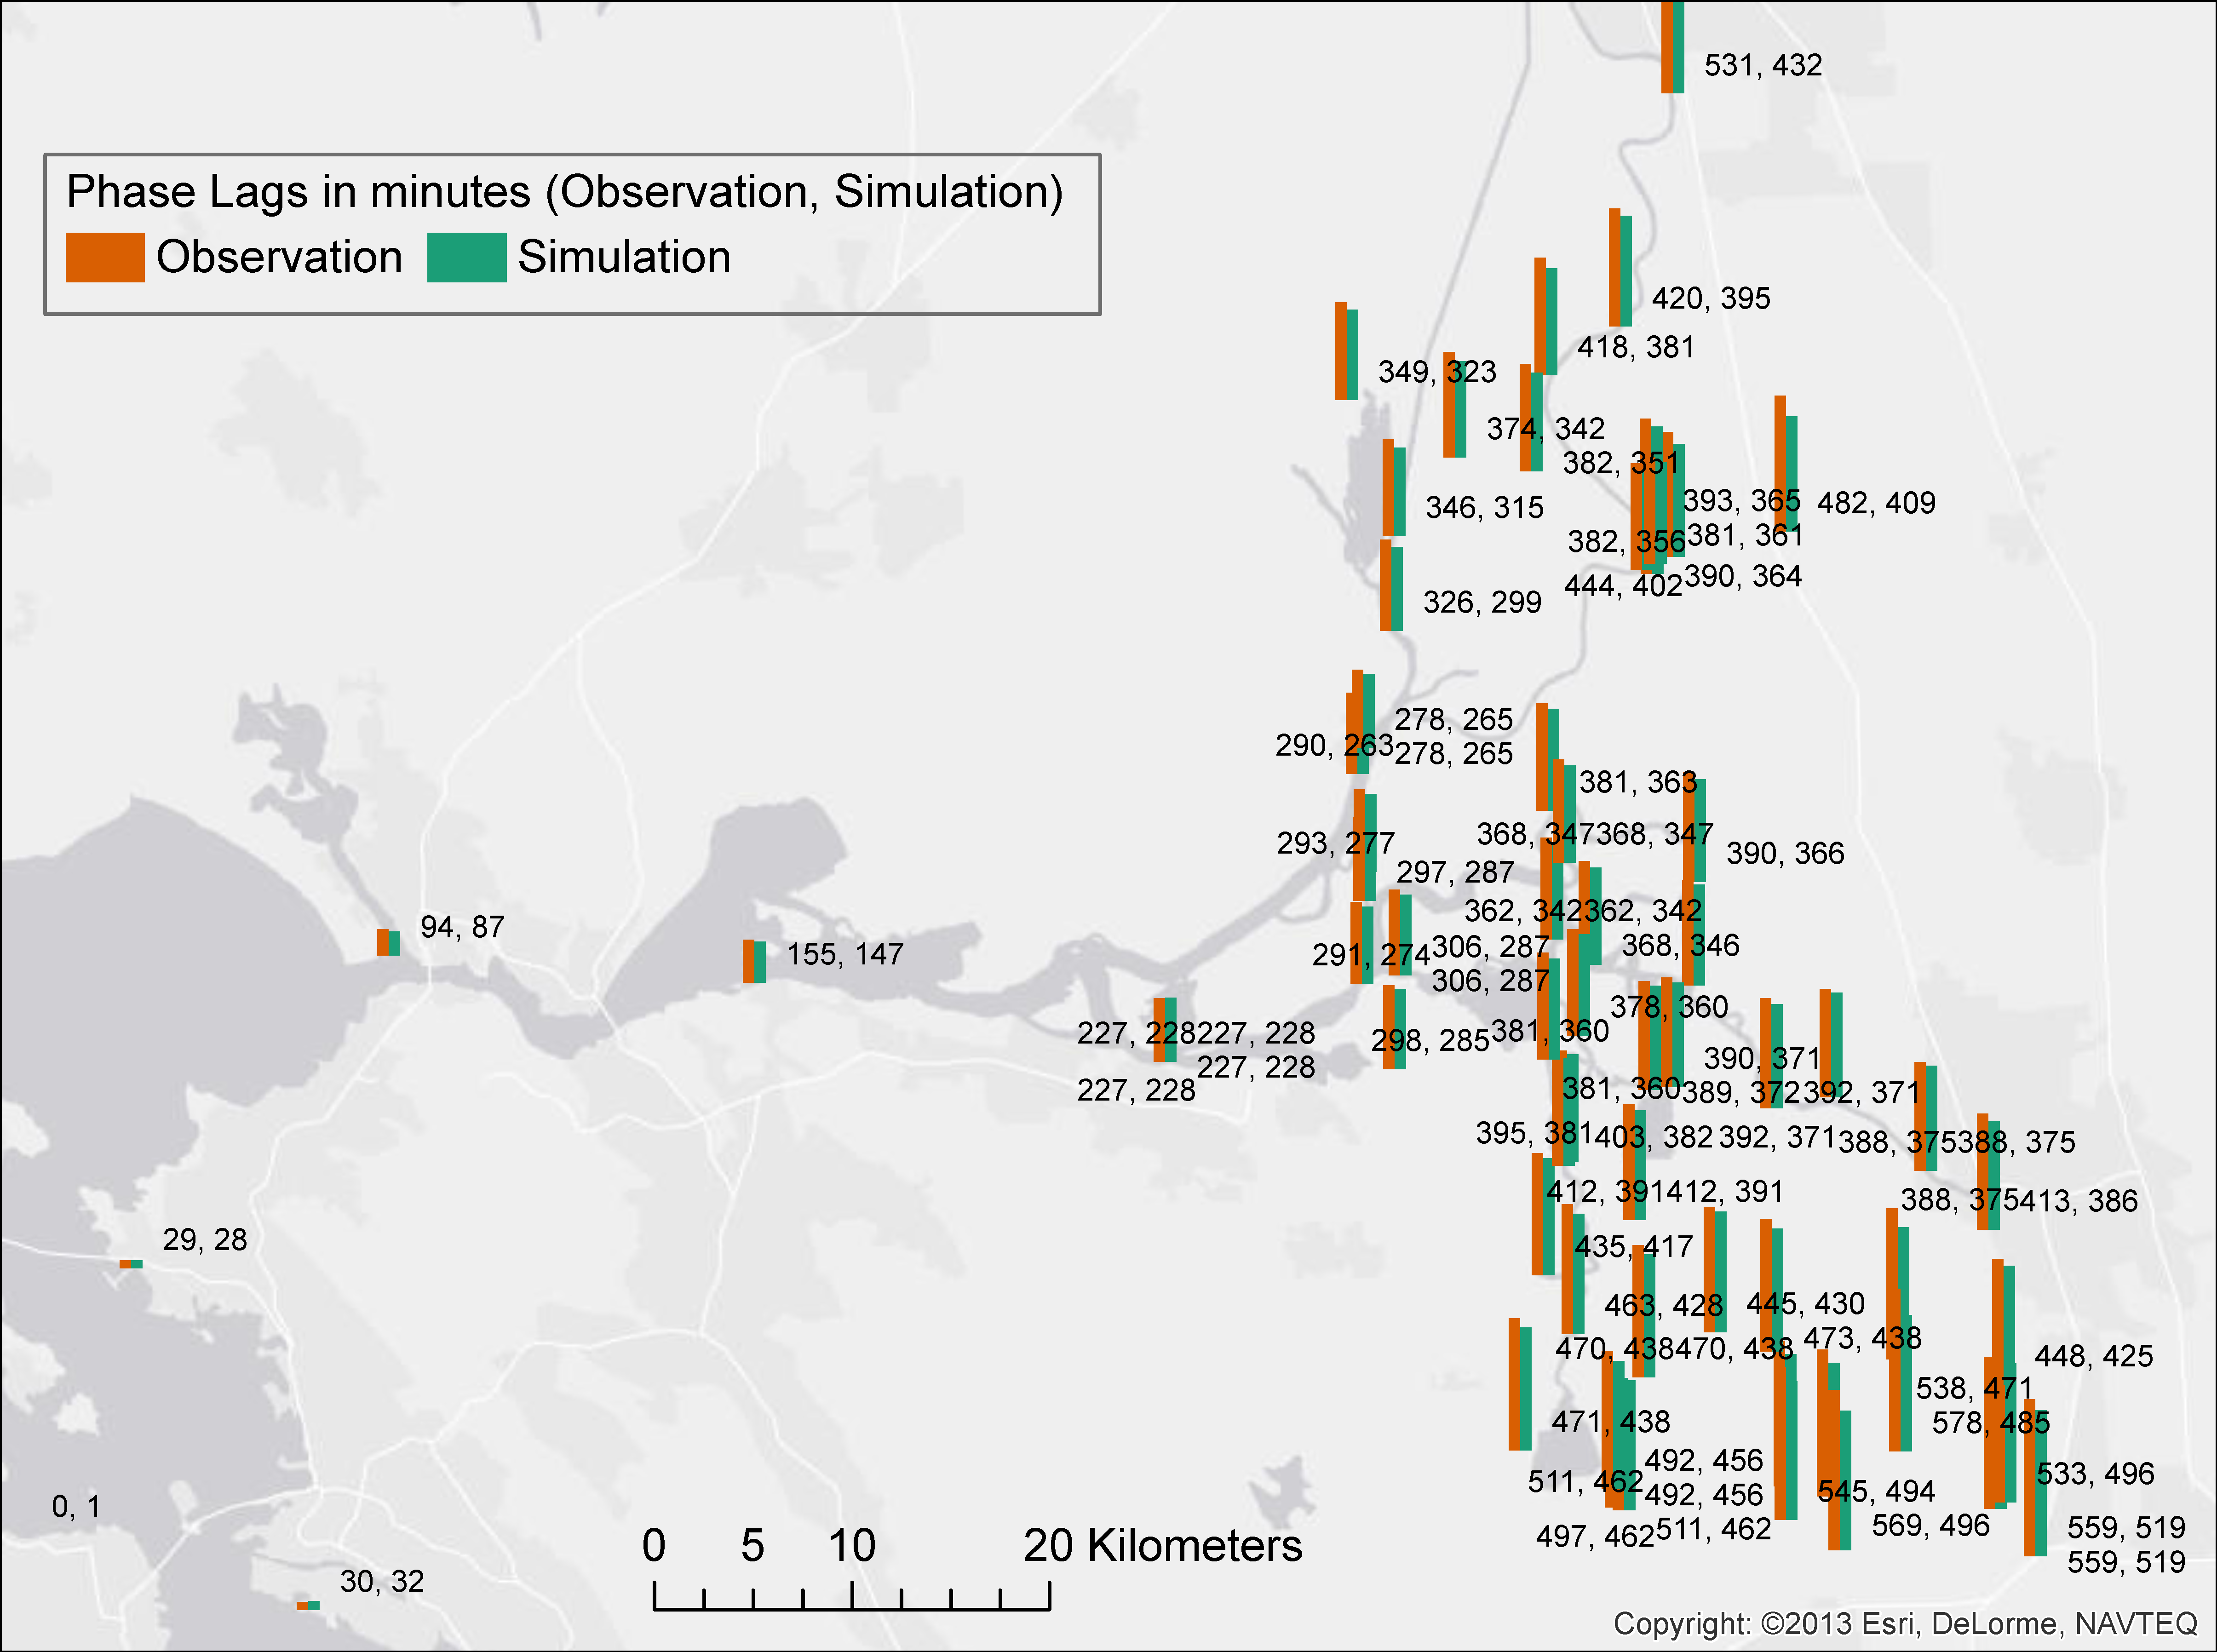
\includegraphics[width=\textwidth]{image/M2_phase_min_spatial}
	\caption{Map of M2 phase at Bay-Delta stations.}
	\label{fig:m2_phase}
\end{figure}
\begin{figure}
	\centering
		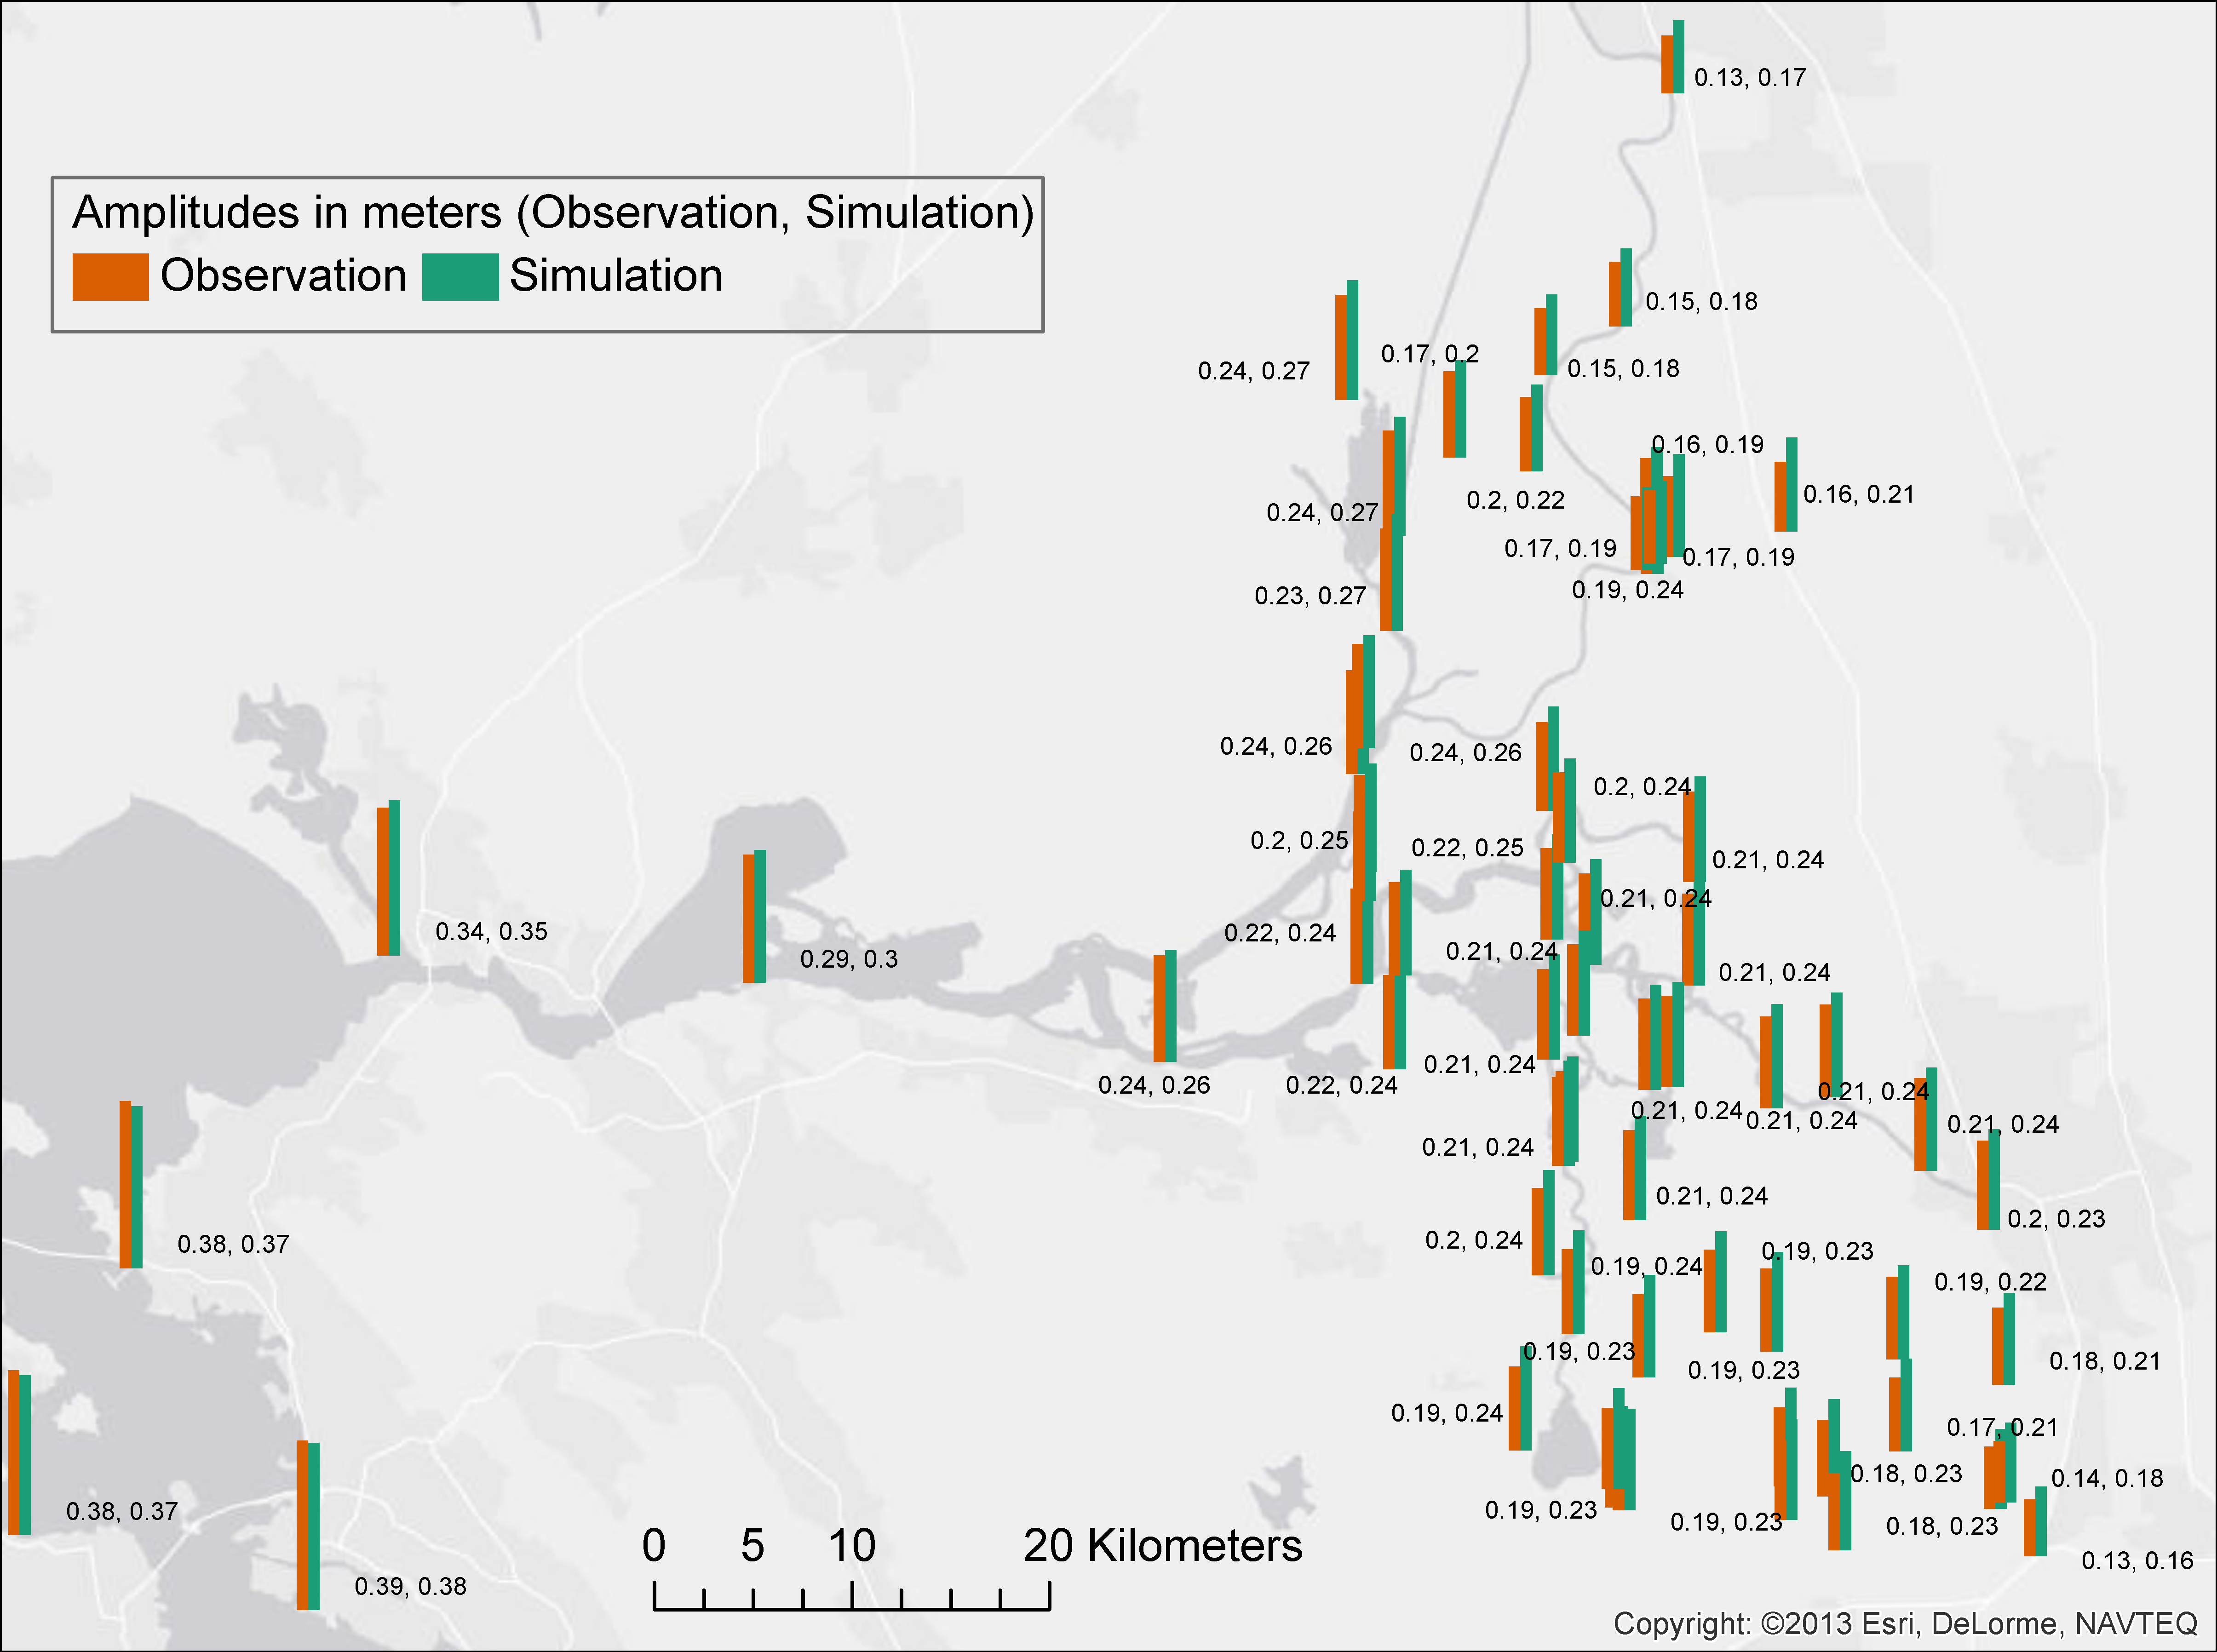
\includegraphics[width=\textwidth]{image/K1_amp_spatial}
	\caption{Map of K1 amplitude at Bay-Delta stations.}
	\label{fig:k1_amp}
\end{figure}
\begin{figure}
	\centering
		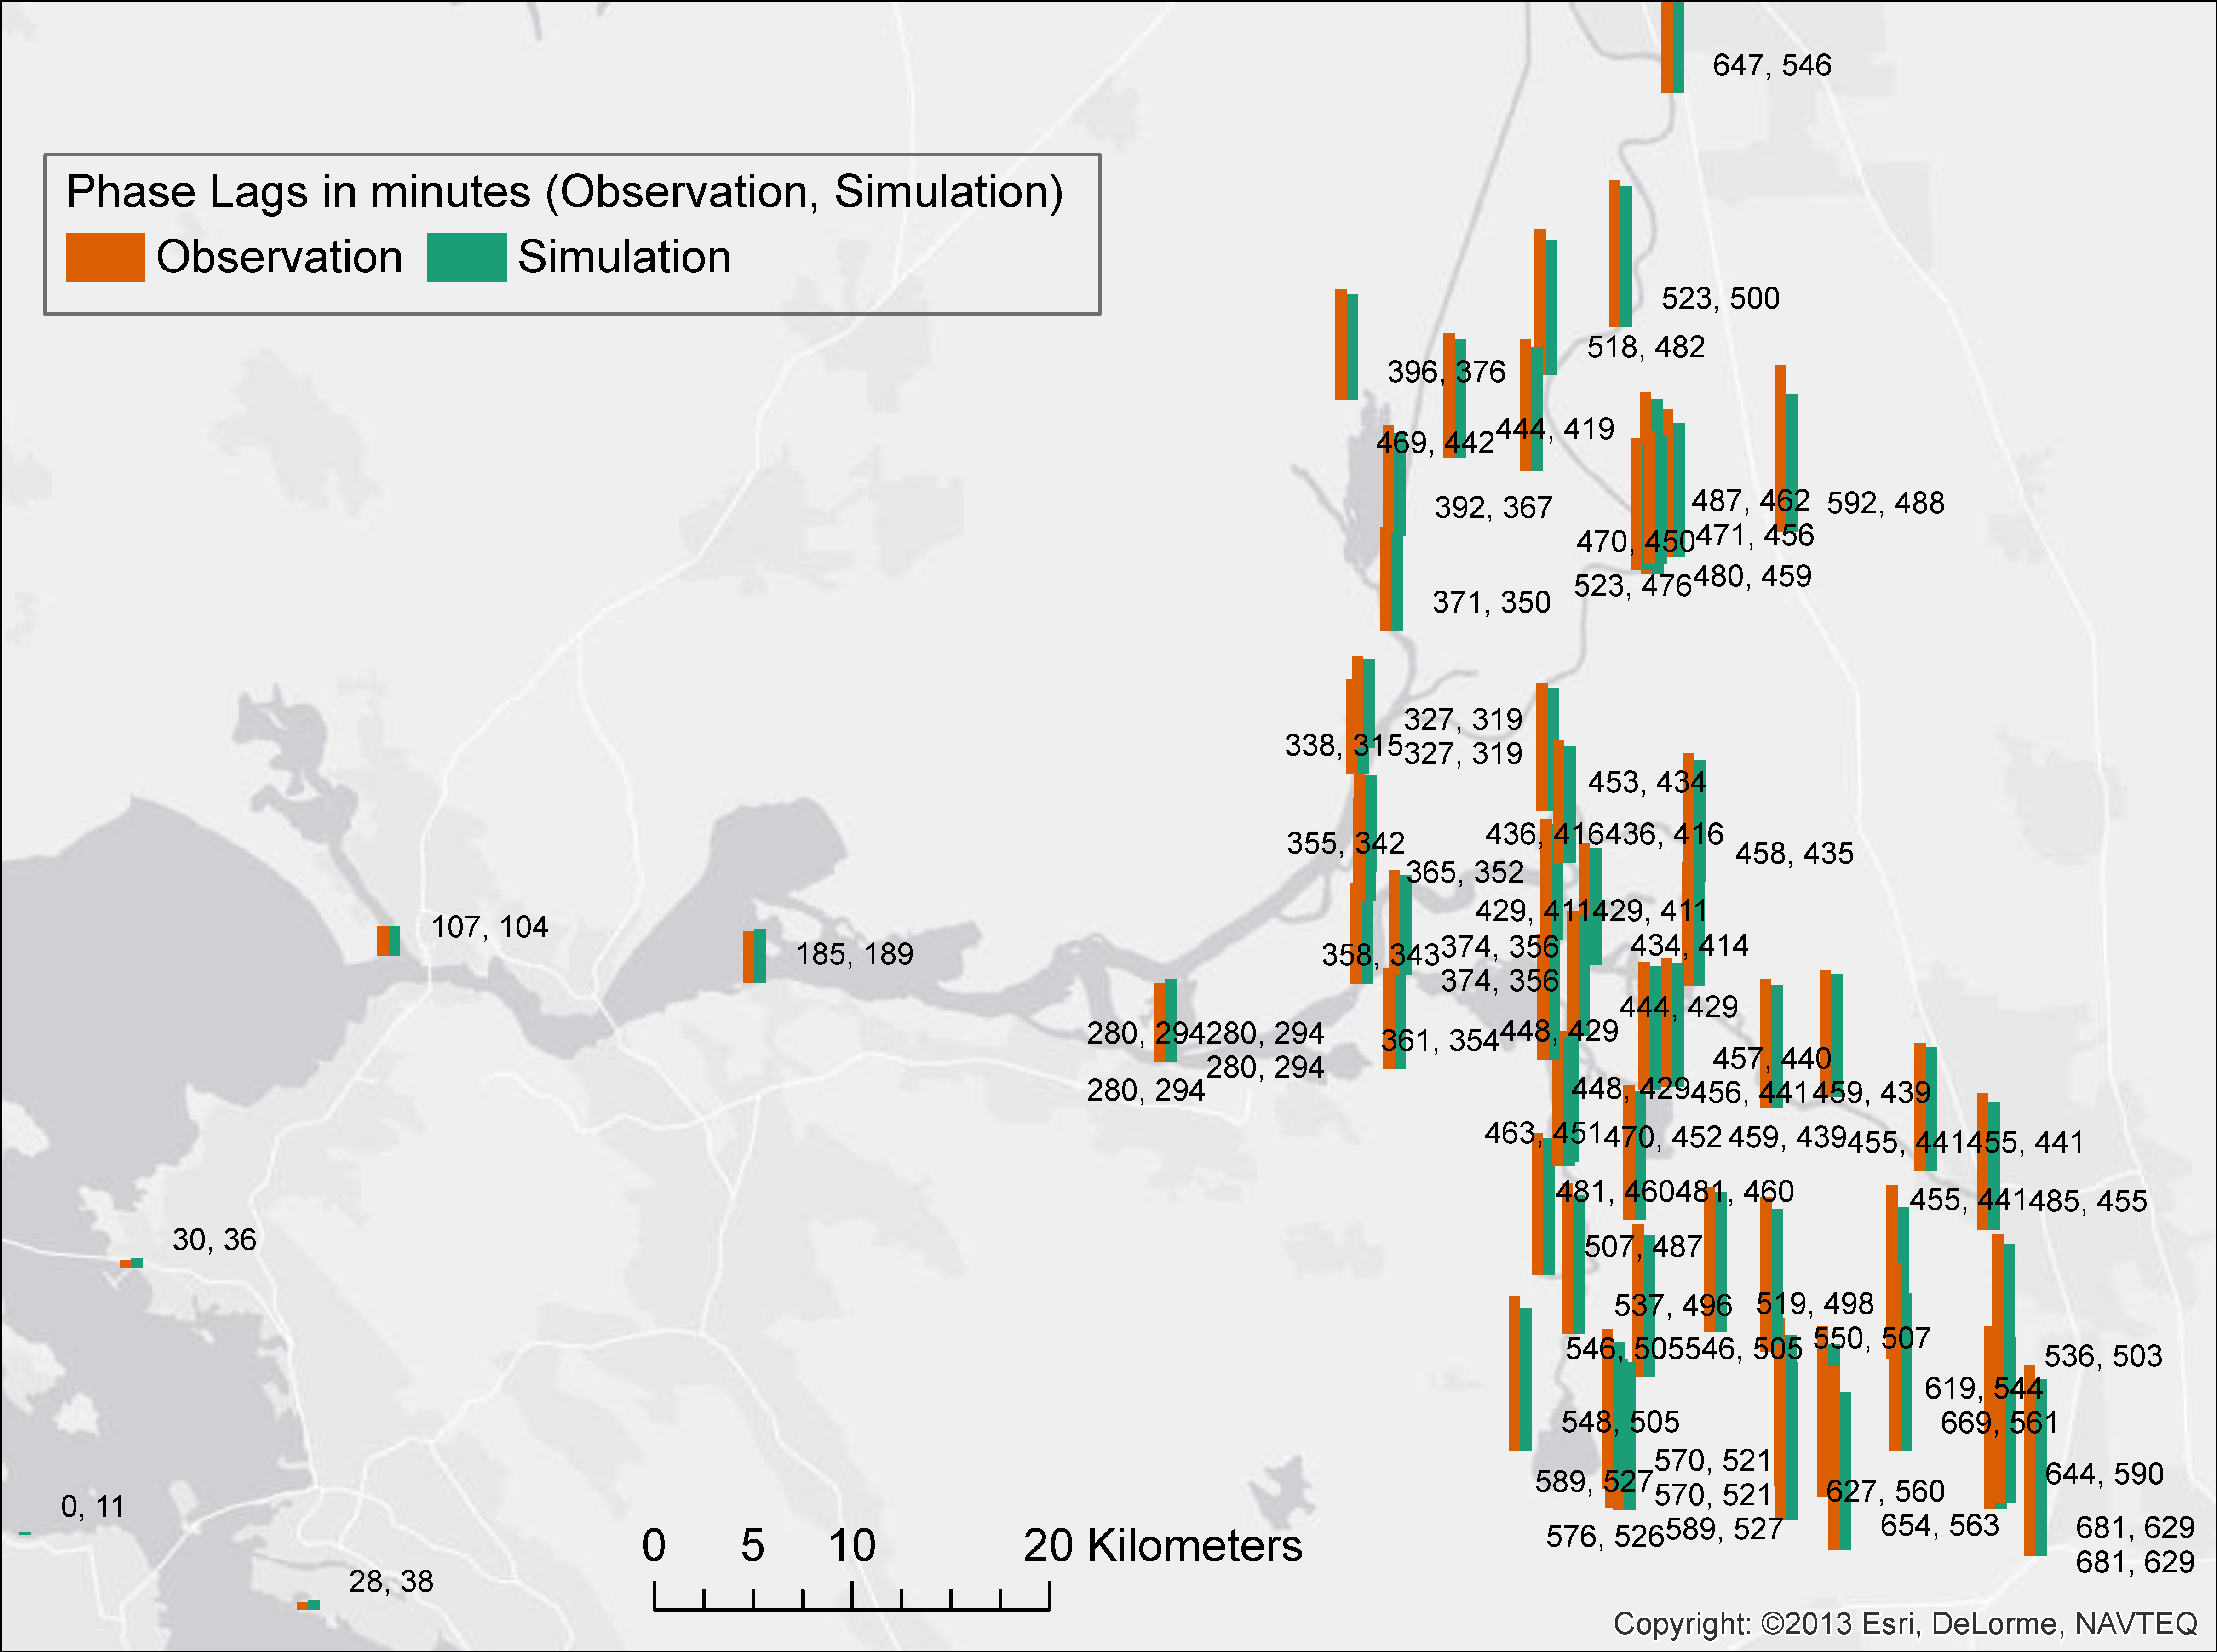
\includegraphics[width=\textwidth]{image/K1_phase_min_spatial}
	\caption{Map of K1 phase at Bay-Delta stations.}
	\label{fig:k1_phase}
\end{figure}

		
		
\section{Flow Results}
  \subsection{Monitoring stations}
	\subsection{Net flow maps} Net flow maps help give a synoptic view of circulation in the Delta. 
	{\em Net flow} here refers to residual flows after filtering to eliminate tidal frequencies 
	or spring-neap variation. Residual flow is of some direct interest because it can contribute 
	to transport and residence time in the Delta -- though this contribution can . 
	Residual flow is also a diagnostic of how well we can model the details of tidal processes,
	since residual flow often manifests as small systematic asymmetries over a (much larger) tidal pattern. 
	
Figures \ref{fig:resid_north_may}-\ref{fig:resid_south_may} compare model and observed mean flow in the North, Central and South Delta for the month of May, 2009. The averages are taken over one month in order to span a spring neap cycle. Barriers have not been installed at this time in the South Delta.

  The general agreement of model with observations is good, although there are some discrepancies
	in the Franks Tract region. Much of the disagreement has to do
	with the routing of residual flow through Dutch Slough versus Jersey Point. The Dutch Slough
	station AFFRA flow meter in place between May and November 2009 was problematic and was replaced 
	after only six months of deployment.
	
	Many of these issues affect observed data as well. In their calibration document, \cite{RMA05} 
	note that mass balance checks around Franks Tract often have discrepancies of 25 cms (roughly 1000 cfs).
	There is nothing about the DWR or USGS data collection processes that considers mass balance, and the 
	net flow is often a somewhat 
	
	
	since 
	and our
	own flow balances calculations agree with the remarks of \cite{RMA05} that observed 
	
	
\begin{figure}
	\centering
		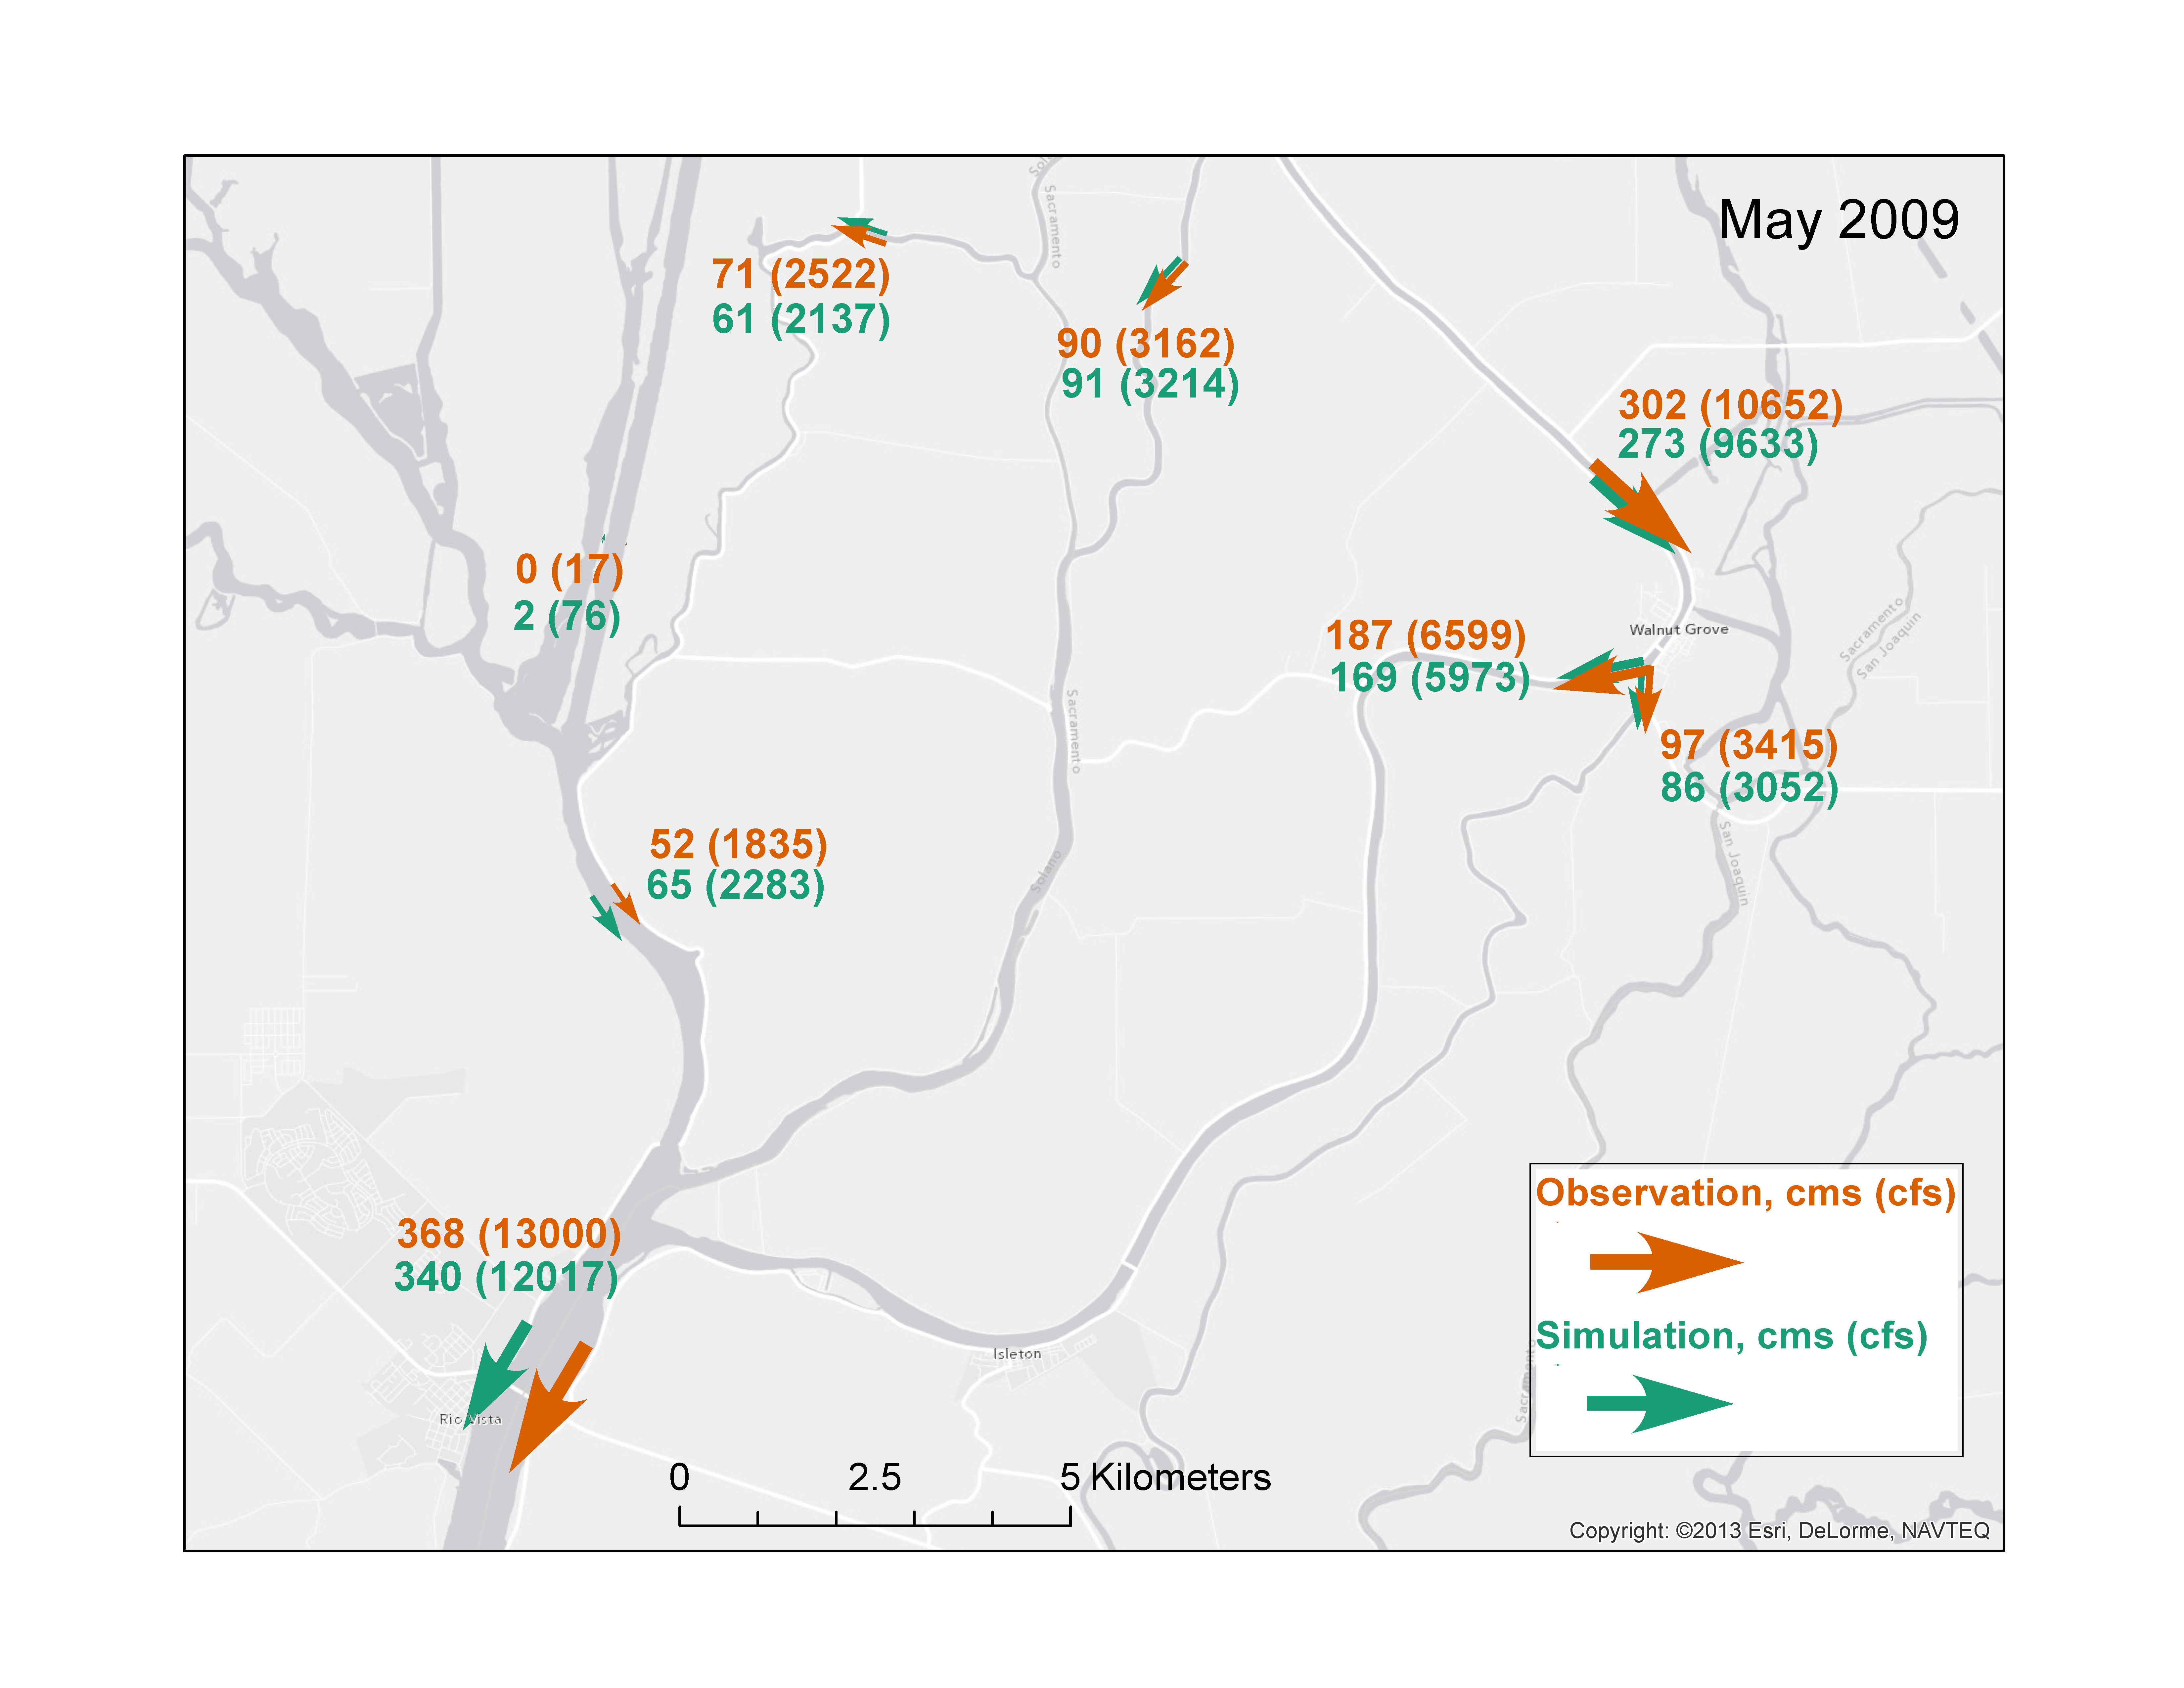
\includegraphics[width=\textwidth]{image/residual_flow_north_delta_64a_may}
	\caption{North Delta monthly residual flow, May 2009. Units are cms (cfs in parentheses).}
	\label{fig:resid_north_may}
\end{figure}

	
\begin{figure}
	\centering
		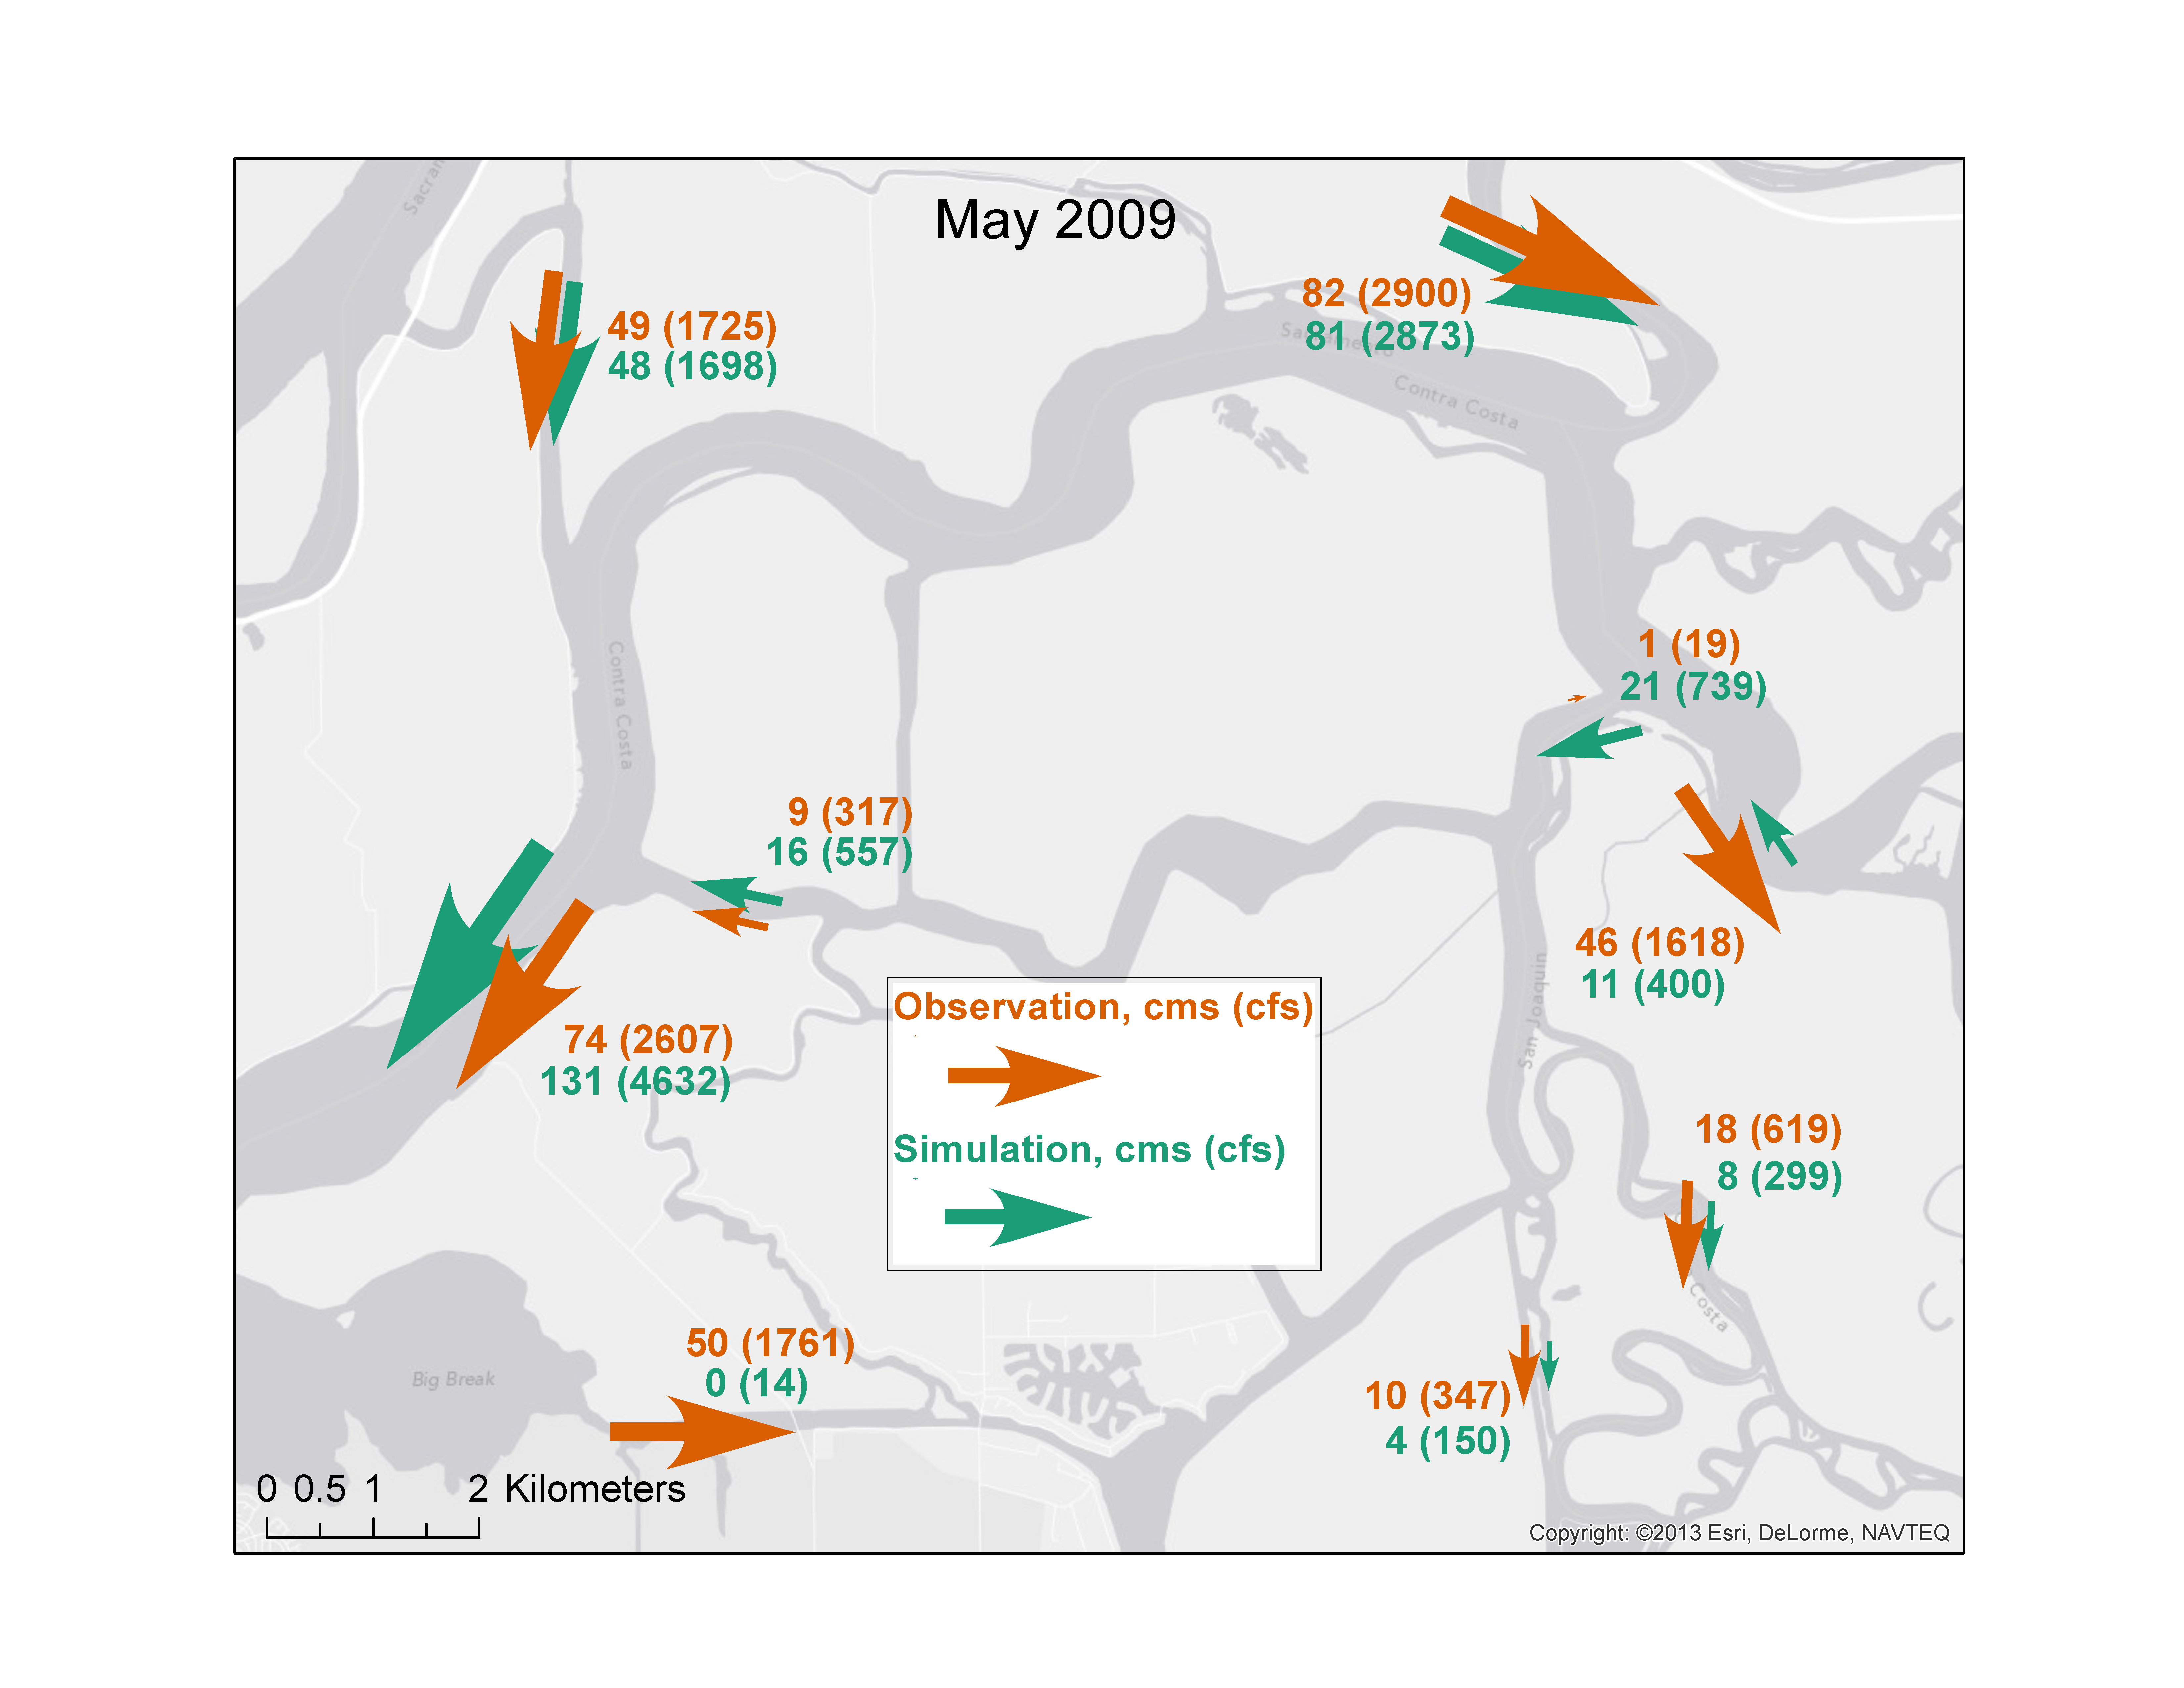
\includegraphics[width=\textwidth]{image/residual_flow_central_delta_64a_may}
	\caption{Central Delta monthly residual flow, May 2009. Units are cms (cfs in parentheses).}
	\label{fig:resid_central_may}
\end{figure}

\begin{figure}
	\centering
		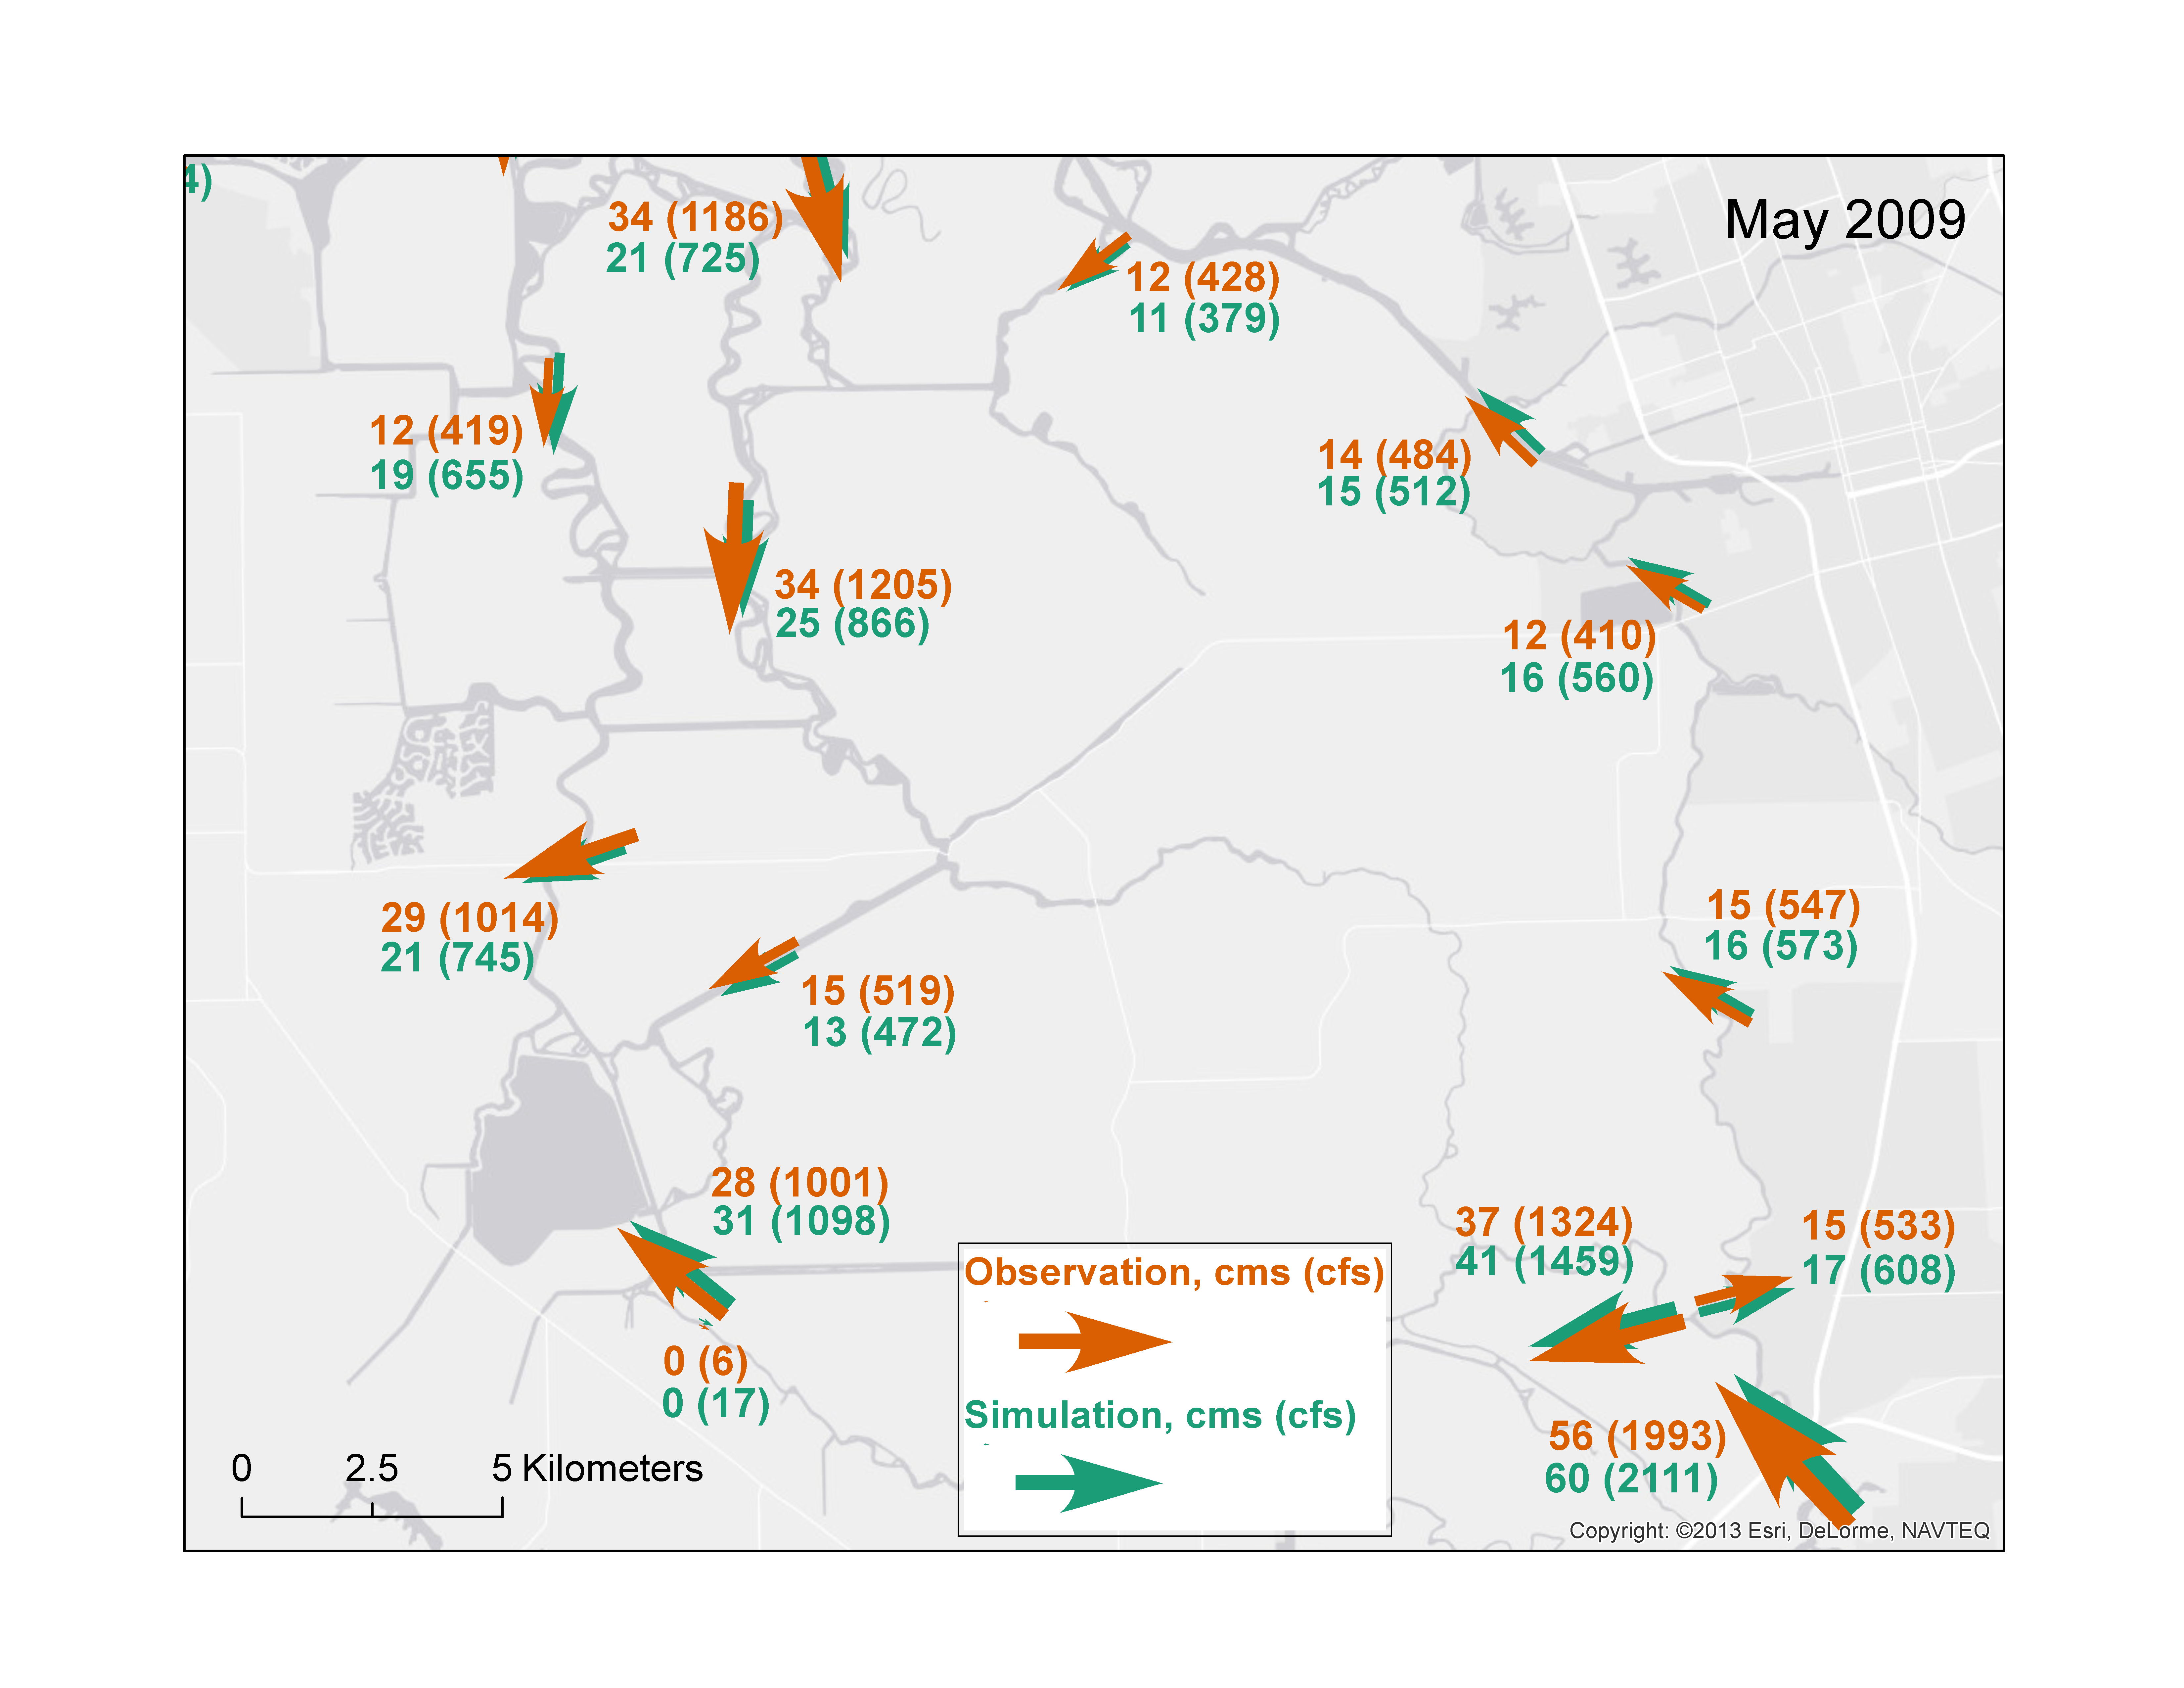
\includegraphics[width=\textwidth]{image/residual_flow_south_delta_64a_may}
	\caption{South Delta monthly residual flow, May 2009. Units are cms (cfs in parentheses).}
	\label{fig:resid_south_may}
\end{figure}
	
\section{Salinity Results}
  \subsection{Monitoring stations}
  \subsection{Surface-bottom stratification}
	\subsection{USGS Cruise CTD casts}

\section{Model sensitivity}
  \subsection{Mesh alteration}
	\subsection{Mesh refinement}
	\subsection{Friction change}
	\subsection{Mass conservation}
  \subsection{Vertical closure}
	\subsection{Atmospheric input}
	\subsection{Boundary Reflection}
  \subsection{Upper water surface and vel flareups}
\chapter{Validation}
The purpose of model validation is to assess, model accuracy. This is typically
done in a different setting than the calibration calibrated. The plots and metrics are largely identical to those introduced in 
\label{chap:validate}. The main differences are the period and selection of station data.

\section{Period of Validation}
The validation is a continuation of the 2009 simulation through *** 2011. Essentially, this is just a
continuation of the calibration simulation. No new field initial conditions are required -- we used the
stopping state of the calibration and allowed a suitable gap of *** to decouple the two period. 
Personnel carrying out the validation were the same as those doing the calibration, but the  
validation component was assembled and analyzed after the calibration was complete.

The validation period brings the model into contact with a slightly wider range of hydrology and
different gate ops ****. The validation also introduces some stations that were previously underutilized. 
Most notably, starting in late 2010 we were able to incorporate midstream USGS water quality 
instruments that were installed at flow stations starting in 2010. We also made more extensive use of USBR 
stations in the validation not because these data are better*** but because
we only acquired certified data for these sites late in the project (we had access through CDEC previous to that
but  as well as USBR stations that, while long-running, 


\section{Stage results}
\section{Flow results}
	\subsection{Flow station data}
	\subsection{Tidal phase and amplitude}
	\subsection{Net flow maps}	
	\subsection{HF Radar}
\section{Salinity results}
  \subsection{Salinity station data}
  \subsection{Surface-bottom stratification}
	\subsection{USGS Cruise CTD casts}


\chapter{Conclusions and Statement of Suitability} 
\section{Delta modeling}
\section{Climate change}
\section{Estuary transport}
\section{Overland flow}
\section{Island flooding}

\bibliography{references}
 \bibliographystyle{plainnat}
\printglossaries
\end{document}
